\hypertarget{_lgm___mag_model_info_8h}{
\section{/home/mgh/LanlGeoMag/libLanlGeoMag/Lgm/Lgm\_\-MagModelInfo.h File Reference}
\label{_lgm___mag_model_info_8h}\index{/home/mgh/LanlGeoMag/libLanlGeoMag/Lgm/Lgm\_\-MagModelInfo.h@{/home/mgh/LanlGeoMag/libLanlGeoMag/Lgm/Lgm\_\-MagModelInfo.h}}
}
{\tt \#include $<$math.h$>$}\par
{\tt \#include \char`\"{}Lgm\_\-QuadPack.h\char`\"{}}\par
{\tt \#include \char`\"{}Lgm\_\-CTrans.h\char`\"{}}\par
{\tt \#include \char`\"{}Lgm\_\-Octree.h\char`\"{}}\par
{\tt \#include \char`\"{}gsl/gsl\_\-errno.h\char`\"{}}\par
{\tt \#include \char`\"{}gsl/gsl\_\-spline.h\char`\"{}}\par


Include dependency graph for Lgm\_\-MagModelInfo.h:\nopagebreak
\begin{figure}[H]
\begin{center}
\leavevmode
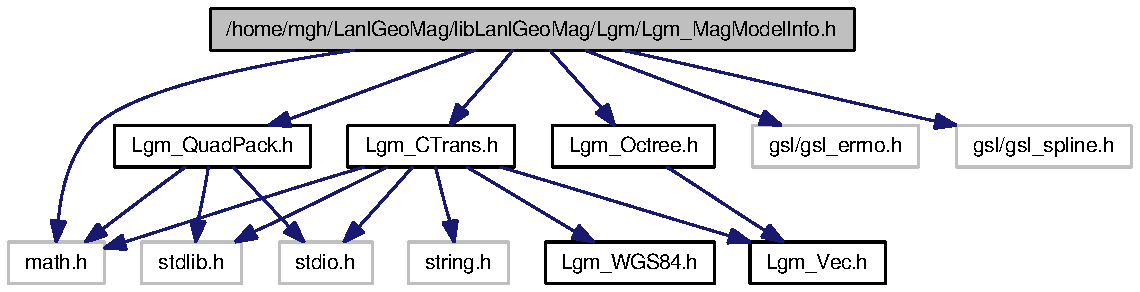
\includegraphics[width=291pt]{_lgm___mag_model_info_8h__incl}
\end{center}
\end{figure}


This graph shows which files directly or indirectly include this file:\nopagebreak
\begin{figure}[H]
\begin{center}
\leavevmode
\includegraphics[width=420pt]{_lgm___mag_model_info_8h__dep__incl}
\end{center}
\end{figure}
\subsection*{Data Structures}
\begin{CompactItemize}
\item 
struct \hyperlink{struct_lgm___mag_model_info}{Lgm\_\-MagModelInfo}
\end{CompactItemize}
\subsection*{Defines}
\begin{CompactItemize}
\item 
\#define \hyperlink{_lgm___mag_model_info_8h_1f6f907234204d7207579a18fb0847a4}{ELECTRON\_\-MASS}~(9.10938188e-31)
\item 
\#define \hyperlink{_lgm___mag_model_info_8h_e72e484b3bba78248e0f70f47d11cb43}{AMU}~(1.660538e-27)
\item 
\#define \hyperlink{_lgm___mag_model_info_8h_b8cacd34cfff7982e36652a0330d8d83}{PROTON\_\-MASS}~(1.00794$\ast$AMU)
\item 
\#define \hyperlink{_lgm___mag_model_info_8h_d6cde5694a5a86aafb92eecd7cf439be}{OXYGEN\_\-MASS}~(15.9994$\ast$AMU)
\item 
\#define \hyperlink{_lgm___mag_model_info_8h_0600e3f227b6e9a3ae26f4d6e2a0581e}{RE}~(6378.135e3)
\item 
\#define \hyperlink{_lgm___mag_model_info_8h_78d126676907aa89a0adbfbef8282585}{CC}~(2.99792458e8)
\item 
\#define \hyperlink{_lgm___mag_model_info_8h_40069882b1f09d9463acc3acd7b67708}{EE}~(1.6022e-19)
\item 
\#define \hyperlink{_lgm___mag_model_info_8h_879ca028f4b6818bf3fdbb2616064dc7}{LGM\_\-OPEN\_\-IMF}~0
\item 
\#define \hyperlink{_lgm___mag_model_info_8h_086cb5005ad71650766b7de8019f9b96}{LGM\_\-CLOSED}~1
\item 
\#define \hyperlink{_lgm___mag_model_info_8h_91b17679023455a7326f797c63c2fe61}{LGM\_\-OPEN\_\-N\_\-LOBE}~2
\item 
\#define \hyperlink{_lgm___mag_model_info_8h_9427a3478101068ebeaeb43eb40ac340}{LGM\_\-OPEN\_\-S\_\-LOBE}~3
\item 
\#define \hyperlink{_lgm___mag_model_info_8h_e3d6196e0512011ee6f33fa69cca2e4e}{LGM\_\-INSIDE\_\-EARTH}~-1
\item 
\#define \hyperlink{_lgm___mag_model_info_8h_65a5ef6633118db80d5c8c19fbb323cc}{LGM\_\-TARGET\_\-HEIGHT\_\-UNREACHABLE}~-2
\item 
\#define \hyperlink{_lgm___mag_model_info_8h_d5b4db481b44d6307a8b6dc3e85b873d}{LGM\_\-MAGSTEP\_\-KMAX}~9
\item 
\#define \hyperlink{_lgm___mag_model_info_8h_9b7c14e73f188763e1544bf9e4f02d05}{LGM\_\-MAGSTEP\_\-IMAX}~(LGM\_\-MAGSTEP\_\-KMAX+1)
\item 
\#define \hyperlink{_lgm___mag_model_info_8h_7eec1adf903922507ec1b6d5dc2bb08b}{LGM\_\-MAGSTEP\_\-JMAX}~(LGM\_\-MAGSTEP\_\-KMAX+2)
\item 
\#define \hyperlink{_lgm___mag_model_info_8h_e913297188886161831577817441e5d4}{LGM\_\-MAGSTEP\_\-REDMAX}~1.0e-5
\item 
\#define \hyperlink{_lgm___mag_model_info_8h_1b3d1ffb3ed6c7e73a98e6854adf78db}{LGM\_\-MAGSTEP\_\-REDMIN}~0.7
\item 
\#define \hyperlink{_lgm___mag_model_info_8h_1e61be4d8476e5c73abbce9e1ef231f7}{LGM\_\-MAGSTEP\_\-SCLMAX}~0.1
\item 
\#define \hyperlink{_lgm___mag_model_info_8h_01daceed709a6c9e7d741caf03372715}{LGM\_\-MAGSTEP\_\-SAFE1}~0.25
\item 
\#define \hyperlink{_lgm___mag_model_info_8h_4be7d5f918ef452c7edad5f30abffdfb}{LGM\_\-MAGSTEP\_\-SAFE2}~0.70
\item 
\#define \hyperlink{_lgm___mag_model_info_8h_1737dae17c50f345f8961e934372016b}{DQAGS}~0
\item 
\#define \hyperlink{_lgm___mag_model_info_8h_e037cf3b2ea604c3bfa628f09fea87cb}{DQAGP}~1
\item 
\#define \hyperlink{_lgm___mag_model_info_8h_00514d362b2f19081b21ab1c41820d76}{DQK21}~2
\item 
\#define \hyperlink{_lgm___mag_model_info_8h_c645eb9a88619ee6f5e14c557ab8ef62}{LINEAR}~0
\item 
\#define \hyperlink{_lgm___mag_model_info_8h_fe0bcb4f5f5984cd1a1fe9205afded87}{LINEAR\_\-DFI}~1
\item 
\#define \hyperlink{_lgm___mag_model_info_8h_054549cb0229d255e4b415c9d356ab3f}{QUADRATIC}~2
\item 
\#define \hyperlink{_lgm___mag_model_info_8h_da2cbb945b5861b8e72d0fecefbd0756}{QUADRATIC\_\-DFI}~3
\item 
\#define \hyperlink{_lgm___mag_model_info_8h_19c112120f8e44a79cafd9e47ec1ec34}{NEWTON\_\-INTERP}~4
\item 
\#define \hyperlink{_lgm___mag_model_info_8h_b6f13fde0dbe1964a00fddb14a679f97}{LGM\_\-CDIP}~0
\item 
\#define \hyperlink{_lgm___mag_model_info_8h_2915cc8a7b7bc29fff3e3d1a64b50c8d}{LGM\_\-EDIP}~1
\item 
\#define \hyperlink{_lgm___mag_model_info_8h_527069ce310a6da97d27de0add2d772c}{LGM\_\-IGRF}~2
\item 
\#define \hyperlink{_lgm___mag_model_info_8h_578254e15a1eb09b4e9d39056adacdd4}{LGM\_\-MAX\_\-INTERP\_\-PNTS}~10000
\item 
\#define \hyperlink{_lgm___mag_model_info_8h_82c2f53b51459f60a463d4e6f027e0a4}{LGM\_\-RELATIVE\_\-JUMP\_\-METHOD}~0
\item 
\#define \hyperlink{_lgm___mag_model_info_8h_ca0f5cc6f9511010f7540ce8b09de535}{LGM\_\-ABSOLUTE\_\-JUMP\_\-METHOD}~1
\end{CompactItemize}
\subsection*{Functions}
\begin{CompactItemize}
\item 
\hyperlink{struct_lgm___mag_model_info}{Lgm\_\-MagModelInfo} $\ast$ \hyperlink{_lgm___mag_model_info_8h_4f16baeb21ae293220cd048d7bb8f757}{Lgm\_\-InitMagInfo} ()
\item 
void \hyperlink{_lgm___mag_model_info_8h_87ae57349dac55ae7393b6a168c080b2}{Lgm\_\-FreeMagInfo} (\hyperlink{struct_lgm___mag_model_info}{Lgm\_\-MagModelInfo} $\ast$Info)
\item 
\hyperlink{struct_lgm___mag_model_info}{Lgm\_\-MagModelInfo} $\ast$ \hyperlink{_lgm___mag_model_info_8h_d3b20a753c7c6d9afef944a6cf9880dc}{Lgm\_\-CopyMagInfo} (\hyperlink{struct_lgm___mag_model_info}{Lgm\_\-MagModelInfo} $\ast$s)
\item 
int \hyperlink{_lgm___mag_model_info_8h_8a39a610942825fe168938aaddec20d7}{Lgm\_\-Trace} (\hyperlink{struct_lgm___vector}{Lgm\_\-Vector} $\ast$u, \hyperlink{struct_lgm___vector}{Lgm\_\-Vector} $\ast$v1, \hyperlink{struct_lgm___vector}{Lgm\_\-Vector} $\ast$v2, \hyperlink{struct_lgm___vector}{Lgm\_\-Vector} $\ast$v3, double Height, double TOL1, double TOL2, \hyperlink{struct_lgm___mag_model_info}{Lgm\_\-MagModelInfo} $\ast$Info)
\item 
int \hyperlink{_lgm___mag_model_info_8h_e26694e4b9c3747fea07eadd0142142e}{Lgm\_\-TraceToMinBSurf} (\hyperlink{struct_lgm___vector}{Lgm\_\-Vector} $\ast$, \hyperlink{struct_lgm___vector}{Lgm\_\-Vector} $\ast$, double, double, \hyperlink{struct_lgm___mag_model_info}{Lgm\_\-MagModelInfo} $\ast$)
\item 
int \hyperlink{_lgm___mag_model_info_8h_ae8951bf644962b97b86b6293e7c71c4}{Lgm\_\-TraceToSMEquat} (\hyperlink{struct_lgm___vector}{Lgm\_\-Vector} $\ast$, \hyperlink{struct_lgm___vector}{Lgm\_\-Vector} $\ast$, double, \hyperlink{struct_lgm___mag_model_info}{Lgm\_\-MagModelInfo} $\ast$)
\item 
int \hyperlink{_lgm___mag_model_info_8h_7b45a70ceb729d0b1f485e8aa67bd24f}{Lgm\_\-TraceToEarth} (\hyperlink{struct_lgm___vector}{Lgm\_\-Vector} $\ast$, \hyperlink{struct_lgm___vector}{Lgm\_\-Vector} $\ast$, double, double, double, \hyperlink{struct_lgm___mag_model_info}{Lgm\_\-MagModelInfo} $\ast$)
\item 
int \hyperlink{_lgm___mag_model_info_8h_b4590c6952725d09b17c1433371db4e2}{Lgm\_\-TraceToSphericalEarth} (\hyperlink{struct_lgm___vector}{Lgm\_\-Vector} $\ast$, \hyperlink{struct_lgm___vector}{Lgm\_\-Vector} $\ast$, double, double, double, \hyperlink{struct_lgm___mag_model_info}{Lgm\_\-MagModelInfo} $\ast$)
\item 
int \hyperlink{_lgm___mag_model_info_8h_68681484778e87dde0f6f80a8fee549f}{Lgm\_\-TraceLine} (\hyperlink{struct_lgm___vector}{Lgm\_\-Vector} $\ast$, \hyperlink{struct_lgm___vector}{Lgm\_\-Vector} $\ast$, double, double, double, int, \hyperlink{struct_lgm___mag_model_info}{Lgm\_\-MagModelInfo} $\ast$)
\item 
int \hyperlink{_lgm___mag_model_info_8h_97c791c85beb7f0f5f816f79226b2e2c}{Lgm\_\-TraceLine2} (\hyperlink{struct_lgm___vector}{Lgm\_\-Vector} $\ast$, \hyperlink{struct_lgm___vector}{Lgm\_\-Vector} $\ast$, double, double, double, double, int, \hyperlink{struct_lgm___mag_model_info}{Lgm\_\-MagModelInfo} $\ast$)
\item 
void \hyperlink{_lgm___mag_model_info_8h_069290bbefbad1db8e625b9e8a0d3a5e}{ReplaceFirstPoint} (double s, double B, \hyperlink{struct_lgm___vector}{Lgm\_\-Vector} $\ast$P, \hyperlink{struct_lgm___mag_model_info}{Lgm\_\-MagModelInfo} $\ast$Info)
\item 
void \hyperlink{_lgm___mag_model_info_8h_a82612dffc3edae2b3fce7cb94e435c0}{AddNewPoint} (double s, double B, \hyperlink{struct_lgm___vector}{Lgm\_\-Vector} $\ast$P, \hyperlink{struct_lgm___mag_model_info}{Lgm\_\-MagModelInfo} $\ast$Info)
\item 
void \hyperlink{_lgm___mag_model_info_8h_a7175b98aed0d6f712ca66d532afe450}{InitSpline} (\hyperlink{struct_lgm___mag_model_info}{Lgm\_\-MagModelInfo} $\ast$Info)
\item 
void \hyperlink{_lgm___mag_model_info_8h_e748e444fc7e684dcead584e1d002e8d}{FreeSpline} (\hyperlink{struct_lgm___mag_model_info}{Lgm\_\-MagModelInfo} $\ast$Info)
\item 
int \hyperlink{_lgm___mag_model_info_8h_c00bd91234cdbfb21a2fdf225f257668}{Lgm\_\-TraceToMinRdotB} (\hyperlink{struct_lgm___vector}{Lgm\_\-Vector} $\ast$, \hyperlink{struct_lgm___vector}{Lgm\_\-Vector} $\ast$, double, \hyperlink{struct_lgm___mag_model_info}{Lgm\_\-MagModelInfo} $\ast$)
\item 
int \hyperlink{_lgm___mag_model_info_8h_c4c1efecd6b1db18ee51b1b28cfe82db}{Lgm\_\-TraceIDL} (int, void $\ast$argv\mbox{[}$\,$\mbox{]})
\item 
int \hyperlink{_lgm___mag_model_info_8h_f5875fcc683e532736574a4edf7e8545}{Lgm\_\-TraceToMirrorPoint} (\hyperlink{struct_lgm___vector}{Lgm\_\-Vector} $\ast$u, \hyperlink{struct_lgm___vector}{Lgm\_\-Vector} $\ast$v, double $\ast$Sm, double H0, double Bm, double sgn, double tol, \hyperlink{struct_lgm___mag_model_info}{Lgm\_\-MagModelInfo} $\ast$Info)
\item 
void \hyperlink{_lgm___mag_model_info_8h_24e31c1882021ee661d8afd00d72e726}{Lgm\_\-ModMid} (\hyperlink{struct_lgm___vector}{Lgm\_\-Vector} $\ast$, \hyperlink{struct_lgm___vector}{Lgm\_\-Vector} $\ast$, double, int, double, int($\ast$Mag)(\hyperlink{struct_lgm___vector}{Lgm\_\-Vector} $\ast$, \hyperlink{struct_lgm___vector}{Lgm\_\-Vector} $\ast$, \hyperlink{struct_lgm___mag_model_info}{Lgm\_\-MagModelInfo} $\ast$), \hyperlink{struct_lgm___mag_model_info}{Lgm\_\-MagModelInfo} $\ast$)
\item 
void \hyperlink{_lgm___mag_model_info_8h_1e8a22ce5672e4a4b9a51ca51713408e}{Lgm\_\-RatFunExt} (int, double, \hyperlink{struct_lgm___vector}{Lgm\_\-Vector} $\ast$, \hyperlink{struct_lgm___vector}{Lgm\_\-Vector} $\ast$, \hyperlink{struct_lgm___vector}{Lgm\_\-Vector} $\ast$, \hyperlink{struct_lgm___mag_model_info}{Lgm\_\-MagModelInfo} $\ast$)
\item 
int \hyperlink{_lgm___mag_model_info_8h_0728ceef72ddab59dac1779e455e554f}{Lgm\_\-MagStep} (\hyperlink{struct_lgm___vector}{Lgm\_\-Vector} $\ast$, \hyperlink{struct_lgm___vector}{Lgm\_\-Vector} $\ast$, double, double $\ast$, double $\ast$, double, double, double $\ast$, int $\ast$, int($\ast$Mag)(\hyperlink{struct_lgm___vector}{Lgm\_\-Vector} $\ast$, \hyperlink{struct_lgm___vector}{Lgm\_\-Vector} $\ast$, \hyperlink{struct_lgm___mag_model_info}{Lgm\_\-MagModelInfo} $\ast$), \hyperlink{struct_lgm___mag_model_info}{Lgm\_\-MagModelInfo} $\ast$)
\item 
int \hyperlink{_lgm___mag_model_info_8h_ab7ce7544097d19271704d13d37c95e8}{Lgm\_\-B\_\-igrf} (\hyperlink{struct_lgm___vector}{Lgm\_\-Vector} $\ast$, \hyperlink{struct_lgm___vector}{Lgm\_\-Vector} $\ast$, \hyperlink{struct_lgm___mag_model_info}{Lgm\_\-MagModelInfo} $\ast$)
\item 
int \hyperlink{_lgm___mag_model_info_8h_35a01e17f8707981772eea21f9030af3}{Lgm\_\-B\_\-cdip} (\hyperlink{struct_lgm___vector}{Lgm\_\-Vector} $\ast$, \hyperlink{struct_lgm___vector}{Lgm\_\-Vector} $\ast$, \hyperlink{struct_lgm___mag_model_info}{Lgm\_\-MagModelInfo} $\ast$)
\item 
int \hyperlink{_lgm___mag_model_info_8h_197f94b29b1159e249e52d11d5aec2a8}{Lgm\_\-B\_\-edip} (\hyperlink{struct_lgm___vector}{Lgm\_\-Vector} $\ast$, \hyperlink{struct_lgm___vector}{Lgm\_\-Vector} $\ast$, \hyperlink{struct_lgm___mag_model_info}{Lgm\_\-MagModelInfo} $\ast$)
\item 
int \hyperlink{_lgm___mag_model_info_8h_1beb428d4ab97b15df348423d1721d90}{Lgm\_\-B1\_\-T87} (\hyperlink{struct_lgm___vector}{Lgm\_\-Vector} $\ast$, \hyperlink{struct_lgm___vector}{Lgm\_\-Vector} $\ast$, \hyperlink{struct_lgm___mag_model_info}{Lgm\_\-MagModelInfo} $\ast$)
\item 
int \hyperlink{_lgm___mag_model_info_8h_c500f305bd1f4f0f6bcc61cceb5d300d}{Lgm\_\-B2\_\-T87} (\hyperlink{struct_lgm___vector}{Lgm\_\-Vector} $\ast$, \hyperlink{struct_lgm___vector}{Lgm\_\-Vector} $\ast$, \hyperlink{struct_lgm___mag_model_info}{Lgm\_\-MagModelInfo} $\ast$)
\item 
int \hyperlink{_lgm___mag_model_info_8h_884728ac6b23c4a999599757d9a28197}{Lgm\_\-B3\_\-T87} (\hyperlink{struct_lgm___vector}{Lgm\_\-Vector} $\ast$, \hyperlink{struct_lgm___vector}{Lgm\_\-Vector} $\ast$, \hyperlink{struct_lgm___mag_model_info}{Lgm\_\-MagModelInfo} $\ast$)
\item 
int \hyperlink{_lgm___mag_model_info_8h_642e78d4ec72c24ed023693687d6afb5}{Lgm\_\-B\_\-T87} (\hyperlink{struct_lgm___vector}{Lgm\_\-Vector} $\ast$, \hyperlink{struct_lgm___vector}{Lgm\_\-Vector} $\ast$, \hyperlink{struct_lgm___mag_model_info}{Lgm\_\-MagModelInfo} $\ast$)
\item 
int \hyperlink{_lgm___mag_model_info_8h_51eb3ce38725f6f1b611b47b74d8d831}{Lgm\_\-BM\_\-T89} (\hyperlink{struct_lgm___vector}{Lgm\_\-Vector} $\ast$, \hyperlink{struct_lgm___vector}{Lgm\_\-Vector} $\ast$, \hyperlink{struct_lgm___mag_model_info}{Lgm\_\-MagModelInfo} $\ast$)
\item 
int \hyperlink{_lgm___mag_model_info_8h_da0b31e3edf146da2f49f5088e4a20ba}{Lgm\_\-BT\_\-T89} (\hyperlink{struct_lgm___vector}{Lgm\_\-Vector} $\ast$, \hyperlink{struct_lgm___vector}{Lgm\_\-Vector} $\ast$, \hyperlink{struct_lgm___mag_model_info}{Lgm\_\-MagModelInfo} $\ast$)
\item 
int \hyperlink{_lgm___mag_model_info_8h_a72b7a373be2bb56c91d7f01eb7661ac}{Lgm\_\-BRC\_\-T89} (\hyperlink{struct_lgm___vector}{Lgm\_\-Vector} $\ast$, \hyperlink{struct_lgm___vector}{Lgm\_\-Vector} $\ast$, \hyperlink{struct_lgm___mag_model_info}{Lgm\_\-MagModelInfo} $\ast$)
\item 
int \hyperlink{_lgm___mag_model_info_8h_478fc5100b3c6a41ed6d6f1bfd833834}{Lgm\_\-BC\_\-T89} (\hyperlink{struct_lgm___vector}{Lgm\_\-Vector} $\ast$, \hyperlink{struct_lgm___vector}{Lgm\_\-Vector} $\ast$, \hyperlink{struct_lgm___mag_model_info}{Lgm\_\-MagModelInfo} $\ast$)
\item 
int \hyperlink{_lgm___mag_model_info_8h_6faade3e5c2ee066f5d364c1fb4140bb}{Lgm\_\-B\_\-T89} (\hyperlink{struct_lgm___vector}{Lgm\_\-Vector} $\ast$, \hyperlink{struct_lgm___vector}{Lgm\_\-Vector} $\ast$, \hyperlink{struct_lgm___mag_model_info}{Lgm\_\-MagModelInfo} $\ast$)
\item 
int \hyperlink{_lgm___mag_model_info_8h_6769313ed0ebf3c17cdd0a8491906fc2}{Lgm\_\-B\_\-T96MOD\_\-MGH} (\hyperlink{struct_lgm___vector}{Lgm\_\-Vector} $\ast$v, \hyperlink{struct_lgm___vector}{Lgm\_\-Vector} $\ast$B, \hyperlink{struct_lgm___mag_model_info}{Lgm\_\-MagModelInfo} $\ast$Info)
\item 
void \hyperlink{_lgm___mag_model_info_8h_0a1f7c860cd079e13dedcd24b583bc2b}{lgm\_\-field\_\-t96mod\_\-mgh\_\-} (double $\ast$, double $\ast$, int $\ast$IYEAR, int $\ast$IDAY, int $\ast$IH, int $\ast$IM, double $\ast$SEC, double $\ast$X, double $\ast$Y, double $\ast$Z, double $\ast$BX, double $\ast$BY, double $\ast$BZ)
\item 
void \hyperlink{_lgm___mag_model_info_8h_e0318c11d75b1133fb52b4393fbe2bea}{lgm\_\-field\_\-t96mod\_\-mgh\_\-\_\-} (double $\ast$PARMOD, double $\ast$AMDF, int $\ast$IYEAR, int $\ast$IDAY, int $\ast$IH, int $\ast$IM, double $\ast$SEC, double $\ast$X, double $\ast$Y, double $\ast$Z, double $\ast$BX, double $\ast$BY, double $\ast$BZ)
\item 
void \hyperlink{_lgm___mag_model_info_8h_2f5583de2b17ada857e7b8d4a50c1c16}{lgm\_\-field\_\-t96mod\_\-} (int $\ast$, int $\ast$, int $\ast$, int $\ast$, double $\ast$, double $\ast$, double $\ast$, double $\ast$, double $\ast$, double $\ast$, double $\ast$)
\item 
int \hyperlink{_lgm___mag_model_info_8h_59f3922662b5fde2ade3e5e4a30e33ef}{Lgm\_\-B\_\-TS04} (\hyperlink{struct_lgm___vector}{Lgm\_\-Vector} $\ast$v, \hyperlink{struct_lgm___vector}{Lgm\_\-Vector} $\ast$B, \hyperlink{struct_lgm___mag_model_info}{Lgm\_\-MagModelInfo} $\ast$Info)
\item 
void \hyperlink{_lgm___mag_model_info_8h_0f1aa5cd2fad03bb25ee03b270849fb3}{Lgm\_\-ComputeW} (double W\mbox{[}$\,$\mbox{]}, int i, double Nk\mbox{[}$\,$\mbox{]}, double Vk\mbox{[}$\,$\mbox{]}, double Bsk\mbox{[}$\,$\mbox{]}, int nk)
\item 
void \hyperlink{_lgm___mag_model_info_8h_54ecb238c46c4acfe5e022e19cc326ec}{Lgm\_\-T04\_\-s} (int IOPT, double $\ast$PARMOD, double PS, double SINPS, double COSPS, double X, double Y, double Z, double $\ast$BX, double $\ast$BY, double $\ast$BZ)
\item 
void \hyperlink{_lgm___mag_model_info_8h_5c047252d169aae0974e5bfed6d71085}{Lgm\_\-EXTERN} (int IOPGEN, int IOPT, int IOPB, int IOPR, double $\ast$A, int NTOT, double PDYN, double DST, double BXIMF, double BYIMF, double BZIMF, double W1, double W2, double W3, double W4, double W5, double W6, double PS, double X, double Y, double Z, double $\ast$BXCF, double $\ast$BYCF, double $\ast$BZCF, double $\ast$BXT1, double $\ast$BYT1, double $\ast$BZT1, double $\ast$BXT2, double $\ast$BYT2, double $\ast$BZT2, double $\ast$BXSRC, double $\ast$BYSRC, double $\ast$BZSRC, double $\ast$BXPRC, double $\ast$BYPRC, double $\ast$BZPRC, double $\ast$BXR11, double $\ast$BYR11, double $\ast$BZR11, double $\ast$BXR12, double $\ast$BYR12, double $\ast$BZR12, double $\ast$BXR21, double $\ast$BYR21, double $\ast$BZR21, double $\ast$BXR22, double $\ast$BYR22, double $\ast$BZR22, double $\ast$HXIMF, double $\ast$HYIMF, double $\ast$HZIMF, double $\ast$BBX, double $\ast$BBY, double $\ast$BBZ)
\item 
int \hyperlink{_lgm___mag_model_info_8h_5138e7f3fa8a67aa8ab528ba9cd606d2}{Lgm\_\-B\_\-FromScatteredData} (\hyperlink{struct_lgm___vector}{Lgm\_\-Vector} $\ast$v, \hyperlink{struct_lgm___vector}{Lgm\_\-Vector} $\ast$B, \hyperlink{struct_lgm___mag_model_info}{Lgm\_\-MagModelInfo} $\ast$Info)
\item 
int \hyperlink{_lgm___mag_model_info_8h_89bb4edde36de4c65ad855806e4066b3}{Lgm\_\-SimplifiedMead} (\hyperlink{struct_lgm___vector}{Lgm\_\-Vector} $\ast$v, \hyperlink{struct_lgm___vector}{Lgm\_\-Vector} $\ast$B, \hyperlink{struct_lgm___mag_model_info}{Lgm\_\-MagModelInfo} $\ast$Info)
\item 
double \hyperlink{_lgm___mag_model_info_8h_f6e6b0cd75ad626d41e0ce06cbec7320}{Iinv} (\hyperlink{struct_lgm___mag_model_info}{Lgm\_\-MagModelInfo} $\ast$fInfo)
\item 
double \hyperlink{_lgm___mag_model_info_8h_9378a29574f93271ed37929e9910f6c6}{I\_\-integrand} (double s, \hyperlink{_lgm___quad_pack_8h_01be5a7db8d2fc2ba26ce793d73b6472}{\_\-qpInfo} $\ast$qpInfo)
\item 
double \hyperlink{_lgm___mag_model_info_8h_ea31055ca3f80f4519c263c09ac3e832}{Iinv\_\-interped} (\hyperlink{struct_lgm___mag_model_info}{Lgm\_\-MagModelInfo} $\ast$fInfo)
\item 
double \hyperlink{_lgm___mag_model_info_8h_9a3dcc288db0c9c8153abd181494514e}{I\_\-integrand\_\-interped} (double s, \hyperlink{_lgm___quad_pack_8h_01be5a7db8d2fc2ba26ce793d73b6472}{\_\-qpInfo} $\ast$qpInfo)
\item 
double \hyperlink{_lgm___mag_model_info_8h_64cd517218ca183a56b43dfc1cf7b124}{SbIntegral} (\hyperlink{struct_lgm___mag_model_info}{Lgm\_\-MagModelInfo} $\ast$fInfo)
\item 
double \hyperlink{_lgm___mag_model_info_8h_23dd3716fba7aa838e159dbf9f447dd0}{Sb\_\-integrand} (double s, \hyperlink{_lgm___quad_pack_8h_01be5a7db8d2fc2ba26ce793d73b6472}{\_\-qpInfo} $\ast$qpInfo)
\item 
double \hyperlink{_lgm___mag_model_info_8h_d53ba64293ea16f5d1878d483d62fcd4}{SbIntegral\_\-interped} (\hyperlink{struct_lgm___mag_model_info}{Lgm\_\-MagModelInfo} $\ast$fInfo)
\item 
double \hyperlink{_lgm___mag_model_info_8h_1828b0051c3925909496a0d956bcaab3}{Sb\_\-integrand\_\-interped} (double s, \hyperlink{_lgm___quad_pack_8h_01be5a7db8d2fc2ba26ce793d73b6472}{\_\-qpInfo} $\ast$qpInfo)
\item 
void \hyperlink{_lgm___mag_model_info_8h_a4b45106bd5072e164b5886359166322}{ratint} (double $\ast$xa, double $\ast$ya, int n, double x, double $\ast$y, double $\ast$dy)
\item 
void \hyperlink{_lgm___mag_model_info_8h_6b600a2b7549cca974e23521b0412a67}{polint} (double $\ast$xa, double $\ast$ya, int n, double x, double $\ast$y, double $\ast$dy)
\item 
void \hyperlink{_lgm___mag_model_info_8h_78b06d0a7ba0cb3be1bdf690bf30d21e}{Interp} (double xa\mbox{[}$\,$\mbox{]}, double ya\mbox{[}$\,$\mbox{]}, long int n, double x, double $\ast$y)
\item 
void \hyperlink{_lgm___mag_model_info_8h_0990e5337b30952cae12aac2bacf44b3}{Interp2} (double xa\mbox{[}$\,$\mbox{]}, double ya\mbox{[}$\,$\mbox{]}, long int n, double x, double $\ast$y)
\item 
double \hyperlink{_lgm___mag_model_info_8h_ce6dc7c926ea34e07011fb1167c2d5d0}{LFromIBmM\_\-Hilton} (double I, double Bm, double M)
\item 
double \hyperlink{_lgm___mag_model_info_8h_3daa38ea6b532d0a030fccd7e8f4d79c}{IFromLBmM\_\-Hilton} (double L, double Bm, double M)
\item 
double \hyperlink{_lgm___mag_model_info_8h_4ee011826916a15076f0efa631ec5e77}{LFromIBmM\_\-McIlwain} (double I, double Bm, double M)
\item 
double \hyperlink{_lgm___mag_model_info_8h_7a35eef2fbb725aae4d03d56ba905dcc}{IFromLBmM\_\-McIlwain} (double L, double Bm, double M)
\item 
double \hyperlink{_lgm___mag_model_info_8h_be359d7bc7bae132a2e5bff78da3d9b2}{BofS} (double s, \hyperlink{struct_lgm___mag_model_info}{Lgm\_\-MagModelInfo} $\ast$Info)
\item 
int \hyperlink{_lgm___mag_model_info_8h_d90887c3d7981a285406d4a15192ac44}{SofBm} (double Bm, double $\ast$ss, double $\ast$sn, \hyperlink{struct_lgm___mag_model_info}{Lgm\_\-MagModelInfo} $\ast$Info)
\item 
void \hyperlink{_lgm___mag_model_info_8h_1df3c4796964cae56b6c9bd883d5954b}{Lgm\_\-MagModelInfo\_\-Set\_\-Psw} (double Psw, \hyperlink{struct_lgm___mag_model_info}{Lgm\_\-MagModelInfo} $\ast$m)
\item 
void \hyperlink{_lgm___mag_model_info_8h_07ff6127e39836ffee154fe3b5eab5e9}{Lgm\_\-MagModelInfo\_\-Set\_\-Kp} (double Kp, \hyperlink{struct_lgm___mag_model_info}{Lgm\_\-MagModelInfo} $\ast$m)
\item 
void \hyperlink{_lgm___mag_model_info_8h_c318ccee75354e49cb61fe38ee8d82a4}{Lgm\_\-Set\_\-Octree\_\-kNN\_\-InterpMethod} (\hyperlink{struct_lgm___mag_model_info}{Lgm\_\-MagModelInfo} $\ast$m, int Method)
\item 
void \hyperlink{_lgm___mag_model_info_8h_678acc89e6dd0a339e73cd0016d182a8}{Lgm\_\-Set\_\-Octree\_\-kNN\_\-k} (\hyperlink{struct_lgm___mag_model_info}{Lgm\_\-MagModelInfo} $\ast$m, int k)
\item 
void \hyperlink{_lgm___mag_model_info_8h_dbde452adbe800b5292798a1668dd255}{Lgm\_\-Set\_\-Octree\_\-kNN\_\-MaxDist} (\hyperlink{struct_lgm___mag_model_info}{Lgm\_\-MagModelInfo} $\ast$m, double MaxDist)
\item 
void \hyperlink{_lgm___mag_model_info_8h_9df19c2b1d0c318e81e774c57ced1929}{Lgm\_\-Set\_\-Open\_\-Limits} (\hyperlink{struct_lgm___mag_model_info}{Lgm\_\-MagModelInfo} $\ast$m, double xmin, double xmax, double ymin, double ymax, double zmin, double zmax)
\end{CompactItemize}


\subsection{Define Documentation}
\hypertarget{_lgm___mag_model_info_8h_1f6f907234204d7207579a18fb0847a4}{
\index{Lgm\_\-MagModelInfo.h@{Lgm\_\-MagModelInfo.h}!ELECTRON\_\-MASS@{ELECTRON\_\-MASS}}
\index{ELECTRON\_\-MASS@{ELECTRON\_\-MASS}!Lgm_MagModelInfo.h@{Lgm\_\-MagModelInfo.h}}
\subsubsection[{ELECTRON\_\-MASS}]{\setlength{\rightskip}{0pt plus 5cm}\#define ELECTRON\_\-MASS~(9.10938188e-31)}}
\label{_lgm___mag_model_info_8h_1f6f907234204d7207579a18fb0847a4}




Definition at line 11 of file Lgm\_\-MagModelInfo.h.\hypertarget{_lgm___mag_model_info_8h_e72e484b3bba78248e0f70f47d11cb43}{
\index{Lgm\_\-MagModelInfo.h@{Lgm\_\-MagModelInfo.h}!AMU@{AMU}}
\index{AMU@{AMU}!Lgm_MagModelInfo.h@{Lgm\_\-MagModelInfo.h}}
\subsubsection[{AMU}]{\setlength{\rightskip}{0pt plus 5cm}\#define AMU~(1.660538e-27)}}
\label{_lgm___mag_model_info_8h_e72e484b3bba78248e0f70f47d11cb43}




Definition at line 12 of file Lgm\_\-MagModelInfo.h.\hypertarget{_lgm___mag_model_info_8h_b8cacd34cfff7982e36652a0330d8d83}{
\index{Lgm\_\-MagModelInfo.h@{Lgm\_\-MagModelInfo.h}!PROTON\_\-MASS@{PROTON\_\-MASS}}
\index{PROTON\_\-MASS@{PROTON\_\-MASS}!Lgm_MagModelInfo.h@{Lgm\_\-MagModelInfo.h}}
\subsubsection[{PROTON\_\-MASS}]{\setlength{\rightskip}{0pt plus 5cm}\#define PROTON\_\-MASS~(1.00794$\ast$AMU)}}
\label{_lgm___mag_model_info_8h_b8cacd34cfff7982e36652a0330d8d83}




Definition at line 13 of file Lgm\_\-MagModelInfo.h.\hypertarget{_lgm___mag_model_info_8h_d6cde5694a5a86aafb92eecd7cf439be}{
\index{Lgm\_\-MagModelInfo.h@{Lgm\_\-MagModelInfo.h}!OXYGEN\_\-MASS@{OXYGEN\_\-MASS}}
\index{OXYGEN\_\-MASS@{OXYGEN\_\-MASS}!Lgm_MagModelInfo.h@{Lgm\_\-MagModelInfo.h}}
\subsubsection[{OXYGEN\_\-MASS}]{\setlength{\rightskip}{0pt plus 5cm}\#define OXYGEN\_\-MASS~(15.9994$\ast$AMU)}}
\label{_lgm___mag_model_info_8h_d6cde5694a5a86aafb92eecd7cf439be}




Definition at line 14 of file Lgm\_\-MagModelInfo.h.\hypertarget{_lgm___mag_model_info_8h_0600e3f227b6e9a3ae26f4d6e2a0581e}{
\index{Lgm\_\-MagModelInfo.h@{Lgm\_\-MagModelInfo.h}!RE@{RE}}
\index{RE@{RE}!Lgm_MagModelInfo.h@{Lgm\_\-MagModelInfo.h}}
\subsubsection[{RE}]{\setlength{\rightskip}{0pt plus 5cm}\#define RE~(6378.135e3)}}
\label{_lgm___mag_model_info_8h_0600e3f227b6e9a3ae26f4d6e2a0581e}




Definition at line 15 of file Lgm\_\-MagModelInfo.h.\hypertarget{_lgm___mag_model_info_8h_78d126676907aa89a0adbfbef8282585}{
\index{Lgm\_\-MagModelInfo.h@{Lgm\_\-MagModelInfo.h}!CC@{CC}}
\index{CC@{CC}!Lgm_MagModelInfo.h@{Lgm\_\-MagModelInfo.h}}
\subsubsection[{CC}]{\setlength{\rightskip}{0pt plus 5cm}\#define CC~(2.99792458e8)}}
\label{_lgm___mag_model_info_8h_78d126676907aa89a0adbfbef8282585}




Definition at line 16 of file Lgm\_\-MagModelInfo.h.\hypertarget{_lgm___mag_model_info_8h_40069882b1f09d9463acc3acd7b67708}{
\index{Lgm\_\-MagModelInfo.h@{Lgm\_\-MagModelInfo.h}!EE@{EE}}
\index{EE@{EE}!Lgm_MagModelInfo.h@{Lgm\_\-MagModelInfo.h}}
\subsubsection[{EE}]{\setlength{\rightskip}{0pt plus 5cm}\#define EE~(1.6022e-19)}}
\label{_lgm___mag_model_info_8h_40069882b1f09d9463acc3acd7b67708}




Definition at line 17 of file Lgm\_\-MagModelInfo.h.\hypertarget{_lgm___mag_model_info_8h_879ca028f4b6818bf3fdbb2616064dc7}{
\index{Lgm\_\-MagModelInfo.h@{Lgm\_\-MagModelInfo.h}!LGM\_\-OPEN\_\-IMF@{LGM\_\-OPEN\_\-IMF}}
\index{LGM\_\-OPEN\_\-IMF@{LGM\_\-OPEN\_\-IMF}!Lgm_MagModelInfo.h@{Lgm\_\-MagModelInfo.h}}
\subsubsection[{LGM\_\-OPEN\_\-IMF}]{\setlength{\rightskip}{0pt plus 5cm}\#define LGM\_\-OPEN\_\-IMF~0}}
\label{_lgm___mag_model_info_8h_879ca028f4b6818bf3fdbb2616064dc7}




Definition at line 31 of file Lgm\_\-MagModelInfo.h.\hypertarget{_lgm___mag_model_info_8h_086cb5005ad71650766b7de8019f9b96}{
\index{Lgm\_\-MagModelInfo.h@{Lgm\_\-MagModelInfo.h}!LGM\_\-CLOSED@{LGM\_\-CLOSED}}
\index{LGM\_\-CLOSED@{LGM\_\-CLOSED}!Lgm_MagModelInfo.h@{Lgm\_\-MagModelInfo.h}}
\subsubsection[{LGM\_\-CLOSED}]{\setlength{\rightskip}{0pt plus 5cm}\#define LGM\_\-CLOSED~1}}
\label{_lgm___mag_model_info_8h_086cb5005ad71650766b7de8019f9b96}




Definition at line 32 of file Lgm\_\-MagModelInfo.h.\hypertarget{_lgm___mag_model_info_8h_91b17679023455a7326f797c63c2fe61}{
\index{Lgm\_\-MagModelInfo.h@{Lgm\_\-MagModelInfo.h}!LGM\_\-OPEN\_\-N\_\-LOBE@{LGM\_\-OPEN\_\-N\_\-LOBE}}
\index{LGM\_\-OPEN\_\-N\_\-LOBE@{LGM\_\-OPEN\_\-N\_\-LOBE}!Lgm_MagModelInfo.h@{Lgm\_\-MagModelInfo.h}}
\subsubsection[{LGM\_\-OPEN\_\-N\_\-LOBE}]{\setlength{\rightskip}{0pt plus 5cm}\#define LGM\_\-OPEN\_\-N\_\-LOBE~2}}
\label{_lgm___mag_model_info_8h_91b17679023455a7326f797c63c2fe61}




Definition at line 33 of file Lgm\_\-MagModelInfo.h.\hypertarget{_lgm___mag_model_info_8h_9427a3478101068ebeaeb43eb40ac340}{
\index{Lgm\_\-MagModelInfo.h@{Lgm\_\-MagModelInfo.h}!LGM\_\-OPEN\_\-S\_\-LOBE@{LGM\_\-OPEN\_\-S\_\-LOBE}}
\index{LGM\_\-OPEN\_\-S\_\-LOBE@{LGM\_\-OPEN\_\-S\_\-LOBE}!Lgm_MagModelInfo.h@{Lgm\_\-MagModelInfo.h}}
\subsubsection[{LGM\_\-OPEN\_\-S\_\-LOBE}]{\setlength{\rightskip}{0pt plus 5cm}\#define LGM\_\-OPEN\_\-S\_\-LOBE~3}}
\label{_lgm___mag_model_info_8h_9427a3478101068ebeaeb43eb40ac340}




Definition at line 34 of file Lgm\_\-MagModelInfo.h.\hypertarget{_lgm___mag_model_info_8h_e3d6196e0512011ee6f33fa69cca2e4e}{
\index{Lgm\_\-MagModelInfo.h@{Lgm\_\-MagModelInfo.h}!LGM\_\-INSIDE\_\-EARTH@{LGM\_\-INSIDE\_\-EARTH}}
\index{LGM\_\-INSIDE\_\-EARTH@{LGM\_\-INSIDE\_\-EARTH}!Lgm_MagModelInfo.h@{Lgm\_\-MagModelInfo.h}}
\subsubsection[{LGM\_\-INSIDE\_\-EARTH}]{\setlength{\rightskip}{0pt plus 5cm}\#define LGM\_\-INSIDE\_\-EARTH~-1}}
\label{_lgm___mag_model_info_8h_e3d6196e0512011ee6f33fa69cca2e4e}




Definition at line 35 of file Lgm\_\-MagModelInfo.h.\hypertarget{_lgm___mag_model_info_8h_65a5ef6633118db80d5c8c19fbb323cc}{
\index{Lgm\_\-MagModelInfo.h@{Lgm\_\-MagModelInfo.h}!LGM\_\-TARGET\_\-HEIGHT\_\-UNREACHABLE@{LGM\_\-TARGET\_\-HEIGHT\_\-UNREACHABLE}}
\index{LGM\_\-TARGET\_\-HEIGHT\_\-UNREACHABLE@{LGM\_\-TARGET\_\-HEIGHT\_\-UNREACHABLE}!Lgm_MagModelInfo.h@{Lgm\_\-MagModelInfo.h}}
\subsubsection[{LGM\_\-TARGET\_\-HEIGHT\_\-UNREACHABLE}]{\setlength{\rightskip}{0pt plus 5cm}\#define LGM\_\-TARGET\_\-HEIGHT\_\-UNREACHABLE~-2}}
\label{_lgm___mag_model_info_8h_65a5ef6633118db80d5c8c19fbb323cc}




Definition at line 36 of file Lgm\_\-MagModelInfo.h.\hypertarget{_lgm___mag_model_info_8h_d5b4db481b44d6307a8b6dc3e85b873d}{
\index{Lgm\_\-MagModelInfo.h@{Lgm\_\-MagModelInfo.h}!LGM\_\-MAGSTEP\_\-KMAX@{LGM\_\-MAGSTEP\_\-KMAX}}
\index{LGM\_\-MAGSTEP\_\-KMAX@{LGM\_\-MAGSTEP\_\-KMAX}!Lgm_MagModelInfo.h@{Lgm\_\-MagModelInfo.h}}
\subsubsection[{LGM\_\-MAGSTEP\_\-KMAX}]{\setlength{\rightskip}{0pt plus 5cm}\#define LGM\_\-MAGSTEP\_\-KMAX~9}}
\label{_lgm___mag_model_info_8h_d5b4db481b44d6307a8b6dc3e85b873d}




Definition at line 39 of file Lgm\_\-MagModelInfo.h.\hypertarget{_lgm___mag_model_info_8h_9b7c14e73f188763e1544bf9e4f02d05}{
\index{Lgm\_\-MagModelInfo.h@{Lgm\_\-MagModelInfo.h}!LGM\_\-MAGSTEP\_\-IMAX@{LGM\_\-MAGSTEP\_\-IMAX}}
\index{LGM\_\-MAGSTEP\_\-IMAX@{LGM\_\-MAGSTEP\_\-IMAX}!Lgm_MagModelInfo.h@{Lgm\_\-MagModelInfo.h}}
\subsubsection[{LGM\_\-MAGSTEP\_\-IMAX}]{\setlength{\rightskip}{0pt plus 5cm}\#define LGM\_\-MAGSTEP\_\-IMAX~(LGM\_\-MAGSTEP\_\-KMAX+1)}}
\label{_lgm___mag_model_info_8h_9b7c14e73f188763e1544bf9e4f02d05}




Definition at line 40 of file Lgm\_\-MagModelInfo.h.\hypertarget{_lgm___mag_model_info_8h_7eec1adf903922507ec1b6d5dc2bb08b}{
\index{Lgm\_\-MagModelInfo.h@{Lgm\_\-MagModelInfo.h}!LGM\_\-MAGSTEP\_\-JMAX@{LGM\_\-MAGSTEP\_\-JMAX}}
\index{LGM\_\-MAGSTEP\_\-JMAX@{LGM\_\-MAGSTEP\_\-JMAX}!Lgm_MagModelInfo.h@{Lgm\_\-MagModelInfo.h}}
\subsubsection[{LGM\_\-MAGSTEP\_\-JMAX}]{\setlength{\rightskip}{0pt plus 5cm}\#define LGM\_\-MAGSTEP\_\-JMAX~(LGM\_\-MAGSTEP\_\-KMAX+2)}}
\label{_lgm___mag_model_info_8h_7eec1adf903922507ec1b6d5dc2bb08b}




Definition at line 41 of file Lgm\_\-MagModelInfo.h.\hypertarget{_lgm___mag_model_info_8h_e913297188886161831577817441e5d4}{
\index{Lgm\_\-MagModelInfo.h@{Lgm\_\-MagModelInfo.h}!LGM\_\-MAGSTEP\_\-REDMAX@{LGM\_\-MAGSTEP\_\-REDMAX}}
\index{LGM\_\-MAGSTEP\_\-REDMAX@{LGM\_\-MAGSTEP\_\-REDMAX}!Lgm_MagModelInfo.h@{Lgm\_\-MagModelInfo.h}}
\subsubsection[{LGM\_\-MAGSTEP\_\-REDMAX}]{\setlength{\rightskip}{0pt plus 5cm}\#define LGM\_\-MAGSTEP\_\-REDMAX~1.0e-5}}
\label{_lgm___mag_model_info_8h_e913297188886161831577817441e5d4}




Definition at line 42 of file Lgm\_\-MagModelInfo.h.\hypertarget{_lgm___mag_model_info_8h_1b3d1ffb3ed6c7e73a98e6854adf78db}{
\index{Lgm\_\-MagModelInfo.h@{Lgm\_\-MagModelInfo.h}!LGM\_\-MAGSTEP\_\-REDMIN@{LGM\_\-MAGSTEP\_\-REDMIN}}
\index{LGM\_\-MAGSTEP\_\-REDMIN@{LGM\_\-MAGSTEP\_\-REDMIN}!Lgm_MagModelInfo.h@{Lgm\_\-MagModelInfo.h}}
\subsubsection[{LGM\_\-MAGSTEP\_\-REDMIN}]{\setlength{\rightskip}{0pt plus 5cm}\#define LGM\_\-MAGSTEP\_\-REDMIN~0.7}}
\label{_lgm___mag_model_info_8h_1b3d1ffb3ed6c7e73a98e6854adf78db}




Definition at line 43 of file Lgm\_\-MagModelInfo.h.\hypertarget{_lgm___mag_model_info_8h_1e61be4d8476e5c73abbce9e1ef231f7}{
\index{Lgm\_\-MagModelInfo.h@{Lgm\_\-MagModelInfo.h}!LGM\_\-MAGSTEP\_\-SCLMAX@{LGM\_\-MAGSTEP\_\-SCLMAX}}
\index{LGM\_\-MAGSTEP\_\-SCLMAX@{LGM\_\-MAGSTEP\_\-SCLMAX}!Lgm_MagModelInfo.h@{Lgm\_\-MagModelInfo.h}}
\subsubsection[{LGM\_\-MAGSTEP\_\-SCLMAX}]{\setlength{\rightskip}{0pt plus 5cm}\#define LGM\_\-MAGSTEP\_\-SCLMAX~0.1}}
\label{_lgm___mag_model_info_8h_1e61be4d8476e5c73abbce9e1ef231f7}




Definition at line 44 of file Lgm\_\-MagModelInfo.h.\hypertarget{_lgm___mag_model_info_8h_01daceed709a6c9e7d741caf03372715}{
\index{Lgm\_\-MagModelInfo.h@{Lgm\_\-MagModelInfo.h}!LGM\_\-MAGSTEP\_\-SAFE1@{LGM\_\-MAGSTEP\_\-SAFE1}}
\index{LGM\_\-MAGSTEP\_\-SAFE1@{LGM\_\-MAGSTEP\_\-SAFE1}!Lgm_MagModelInfo.h@{Lgm\_\-MagModelInfo.h}}
\subsubsection[{LGM\_\-MAGSTEP\_\-SAFE1}]{\setlength{\rightskip}{0pt plus 5cm}\#define LGM\_\-MAGSTEP\_\-SAFE1~0.25}}
\label{_lgm___mag_model_info_8h_01daceed709a6c9e7d741caf03372715}




Definition at line 45 of file Lgm\_\-MagModelInfo.h.\hypertarget{_lgm___mag_model_info_8h_4be7d5f918ef452c7edad5f30abffdfb}{
\index{Lgm\_\-MagModelInfo.h@{Lgm\_\-MagModelInfo.h}!LGM\_\-MAGSTEP\_\-SAFE2@{LGM\_\-MAGSTEP\_\-SAFE2}}
\index{LGM\_\-MAGSTEP\_\-SAFE2@{LGM\_\-MAGSTEP\_\-SAFE2}!Lgm_MagModelInfo.h@{Lgm\_\-MagModelInfo.h}}
\subsubsection[{LGM\_\-MAGSTEP\_\-SAFE2}]{\setlength{\rightskip}{0pt plus 5cm}\#define LGM\_\-MAGSTEP\_\-SAFE2~0.70}}
\label{_lgm___mag_model_info_8h_4be7d5f918ef452c7edad5f30abffdfb}




Definition at line 46 of file Lgm\_\-MagModelInfo.h.\hypertarget{_lgm___mag_model_info_8h_1737dae17c50f345f8961e934372016b}{
\index{Lgm\_\-MagModelInfo.h@{Lgm\_\-MagModelInfo.h}!DQAGS@{DQAGS}}
\index{DQAGS@{DQAGS}!Lgm_MagModelInfo.h@{Lgm\_\-MagModelInfo.h}}
\subsubsection[{DQAGS}]{\setlength{\rightskip}{0pt plus 5cm}\#define DQAGS~0}}
\label{_lgm___mag_model_info_8h_1737dae17c50f345f8961e934372016b}




Definition at line 48 of file Lgm\_\-MagModelInfo.h.\hypertarget{_lgm___mag_model_info_8h_e037cf3b2ea604c3bfa628f09fea87cb}{
\index{Lgm\_\-MagModelInfo.h@{Lgm\_\-MagModelInfo.h}!DQAGP@{DQAGP}}
\index{DQAGP@{DQAGP}!Lgm_MagModelInfo.h@{Lgm\_\-MagModelInfo.h}}
\subsubsection[{DQAGP}]{\setlength{\rightskip}{0pt plus 5cm}\#define DQAGP~1}}
\label{_lgm___mag_model_info_8h_e037cf3b2ea604c3bfa628f09fea87cb}




Definition at line 49 of file Lgm\_\-MagModelInfo.h.\hypertarget{_lgm___mag_model_info_8h_00514d362b2f19081b21ab1c41820d76}{
\index{Lgm\_\-MagModelInfo.h@{Lgm\_\-MagModelInfo.h}!DQK21@{DQK21}}
\index{DQK21@{DQK21}!Lgm_MagModelInfo.h@{Lgm\_\-MagModelInfo.h}}
\subsubsection[{DQK21}]{\setlength{\rightskip}{0pt plus 5cm}\#define DQK21~2}}
\label{_lgm___mag_model_info_8h_00514d362b2f19081b21ab1c41820d76}




Definition at line 50 of file Lgm\_\-MagModelInfo.h.\hypertarget{_lgm___mag_model_info_8h_c645eb9a88619ee6f5e14c557ab8ef62}{
\index{Lgm\_\-MagModelInfo.h@{Lgm\_\-MagModelInfo.h}!LINEAR@{LINEAR}}
\index{LINEAR@{LINEAR}!Lgm_MagModelInfo.h@{Lgm\_\-MagModelInfo.h}}
\subsubsection[{LINEAR}]{\setlength{\rightskip}{0pt plus 5cm}\#define LINEAR~0}}
\label{_lgm___mag_model_info_8h_c645eb9a88619ee6f5e14c557ab8ef62}




Definition at line 59 of file Lgm\_\-MagModelInfo.h.\hypertarget{_lgm___mag_model_info_8h_fe0bcb4f5f5984cd1a1fe9205afded87}{
\index{Lgm\_\-MagModelInfo.h@{Lgm\_\-MagModelInfo.h}!LINEAR\_\-DFI@{LINEAR\_\-DFI}}
\index{LINEAR\_\-DFI@{LINEAR\_\-DFI}!Lgm_MagModelInfo.h@{Lgm\_\-MagModelInfo.h}}
\subsubsection[{LINEAR\_\-DFI}]{\setlength{\rightskip}{0pt plus 5cm}\#define LINEAR\_\-DFI~1}}
\label{_lgm___mag_model_info_8h_fe0bcb4f5f5984cd1a1fe9205afded87}




Definition at line 60 of file Lgm\_\-MagModelInfo.h.\hypertarget{_lgm___mag_model_info_8h_054549cb0229d255e4b415c9d356ab3f}{
\index{Lgm\_\-MagModelInfo.h@{Lgm\_\-MagModelInfo.h}!QUADRATIC@{QUADRATIC}}
\index{QUADRATIC@{QUADRATIC}!Lgm_MagModelInfo.h@{Lgm\_\-MagModelInfo.h}}
\subsubsection[{QUADRATIC}]{\setlength{\rightskip}{0pt plus 5cm}\#define QUADRATIC~2}}
\label{_lgm___mag_model_info_8h_054549cb0229d255e4b415c9d356ab3f}




Definition at line 61 of file Lgm\_\-MagModelInfo.h.\hypertarget{_lgm___mag_model_info_8h_da2cbb945b5861b8e72d0fecefbd0756}{
\index{Lgm\_\-MagModelInfo.h@{Lgm\_\-MagModelInfo.h}!QUADRATIC\_\-DFI@{QUADRATIC\_\-DFI}}
\index{QUADRATIC\_\-DFI@{QUADRATIC\_\-DFI}!Lgm_MagModelInfo.h@{Lgm\_\-MagModelInfo.h}}
\subsubsection[{QUADRATIC\_\-DFI}]{\setlength{\rightskip}{0pt plus 5cm}\#define QUADRATIC\_\-DFI~3}}
\label{_lgm___mag_model_info_8h_da2cbb945b5861b8e72d0fecefbd0756}




Definition at line 62 of file Lgm\_\-MagModelInfo.h.\hypertarget{_lgm___mag_model_info_8h_19c112120f8e44a79cafd9e47ec1ec34}{
\index{Lgm\_\-MagModelInfo.h@{Lgm\_\-MagModelInfo.h}!NEWTON\_\-INTERP@{NEWTON\_\-INTERP}}
\index{NEWTON\_\-INTERP@{NEWTON\_\-INTERP}!Lgm_MagModelInfo.h@{Lgm\_\-MagModelInfo.h}}
\subsubsection[{NEWTON\_\-INTERP}]{\setlength{\rightskip}{0pt plus 5cm}\#define NEWTON\_\-INTERP~4}}
\label{_lgm___mag_model_info_8h_19c112120f8e44a79cafd9e47ec1ec34}




Definition at line 63 of file Lgm\_\-MagModelInfo.h.\hypertarget{_lgm___mag_model_info_8h_b6f13fde0dbe1964a00fddb14a679f97}{
\index{Lgm\_\-MagModelInfo.h@{Lgm\_\-MagModelInfo.h}!LGM\_\-CDIP@{LGM\_\-CDIP}}
\index{LGM\_\-CDIP@{LGM\_\-CDIP}!Lgm_MagModelInfo.h@{Lgm\_\-MagModelInfo.h}}
\subsubsection[{LGM\_\-CDIP}]{\setlength{\rightskip}{0pt plus 5cm}\#define LGM\_\-CDIP~0}}
\label{_lgm___mag_model_info_8h_b6f13fde0dbe1964a00fddb14a679f97}




Definition at line 65 of file Lgm\_\-MagModelInfo.h.\hypertarget{_lgm___mag_model_info_8h_2915cc8a7b7bc29fff3e3d1a64b50c8d}{
\index{Lgm\_\-MagModelInfo.h@{Lgm\_\-MagModelInfo.h}!LGM\_\-EDIP@{LGM\_\-EDIP}}
\index{LGM\_\-EDIP@{LGM\_\-EDIP}!Lgm_MagModelInfo.h@{Lgm\_\-MagModelInfo.h}}
\subsubsection[{LGM\_\-EDIP}]{\setlength{\rightskip}{0pt plus 5cm}\#define LGM\_\-EDIP~1}}
\label{_lgm___mag_model_info_8h_2915cc8a7b7bc29fff3e3d1a64b50c8d}




Definition at line 66 of file Lgm\_\-MagModelInfo.h.\hypertarget{_lgm___mag_model_info_8h_527069ce310a6da97d27de0add2d772c}{
\index{Lgm\_\-MagModelInfo.h@{Lgm\_\-MagModelInfo.h}!LGM\_\-IGRF@{LGM\_\-IGRF}}
\index{LGM\_\-IGRF@{LGM\_\-IGRF}!Lgm_MagModelInfo.h@{Lgm\_\-MagModelInfo.h}}
\subsubsection[{LGM\_\-IGRF}]{\setlength{\rightskip}{0pt plus 5cm}\#define LGM\_\-IGRF~2}}
\label{_lgm___mag_model_info_8h_527069ce310a6da97d27de0add2d772c}




Definition at line 67 of file Lgm\_\-MagModelInfo.h.\hypertarget{_lgm___mag_model_info_8h_578254e15a1eb09b4e9d39056adacdd4}{
\index{Lgm\_\-MagModelInfo.h@{Lgm\_\-MagModelInfo.h}!LGM\_\-MAX\_\-INTERP\_\-PNTS@{LGM\_\-MAX\_\-INTERP\_\-PNTS}}
\index{LGM\_\-MAX\_\-INTERP\_\-PNTS@{LGM\_\-MAX\_\-INTERP\_\-PNTS}!Lgm_MagModelInfo.h@{Lgm\_\-MagModelInfo.h}}
\subsubsection[{LGM\_\-MAX\_\-INTERP\_\-PNTS}]{\setlength{\rightskip}{0pt plus 5cm}\#define LGM\_\-MAX\_\-INTERP\_\-PNTS~10000}}
\label{_lgm___mag_model_info_8h_578254e15a1eb09b4e9d39056adacdd4}




Definition at line 69 of file Lgm\_\-MagModelInfo.h.\hypertarget{_lgm___mag_model_info_8h_82c2f53b51459f60a463d4e6f027e0a4}{
\index{Lgm\_\-MagModelInfo.h@{Lgm\_\-MagModelInfo.h}!LGM\_\-RELATIVE\_\-JUMP\_\-METHOD@{LGM\_\-RELATIVE\_\-JUMP\_\-METHOD}}
\index{LGM\_\-RELATIVE\_\-JUMP\_\-METHOD@{LGM\_\-RELATIVE\_\-JUMP\_\-METHOD}!Lgm_MagModelInfo.h@{Lgm\_\-MagModelInfo.h}}
\subsubsection[{LGM\_\-RELATIVE\_\-JUMP\_\-METHOD}]{\setlength{\rightskip}{0pt plus 5cm}\#define LGM\_\-RELATIVE\_\-JUMP\_\-METHOD~0}}
\label{_lgm___mag_model_info_8h_82c2f53b51459f60a463d4e6f027e0a4}




Definition at line 71 of file Lgm\_\-MagModelInfo.h.\hypertarget{_lgm___mag_model_info_8h_ca0f5cc6f9511010f7540ce8b09de535}{
\index{Lgm\_\-MagModelInfo.h@{Lgm\_\-MagModelInfo.h}!LGM\_\-ABSOLUTE\_\-JUMP\_\-METHOD@{LGM\_\-ABSOLUTE\_\-JUMP\_\-METHOD}}
\index{LGM\_\-ABSOLUTE\_\-JUMP\_\-METHOD@{LGM\_\-ABSOLUTE\_\-JUMP\_\-METHOD}!Lgm_MagModelInfo.h@{Lgm\_\-MagModelInfo.h}}
\subsubsection[{LGM\_\-ABSOLUTE\_\-JUMP\_\-METHOD}]{\setlength{\rightskip}{0pt plus 5cm}\#define LGM\_\-ABSOLUTE\_\-JUMP\_\-METHOD~1}}
\label{_lgm___mag_model_info_8h_ca0f5cc6f9511010f7540ce8b09de535}




Definition at line 72 of file Lgm\_\-MagModelInfo.h.

\subsection{Function Documentation}
\hypertarget{_lgm___mag_model_info_8h_4f16baeb21ae293220cd048d7bb8f757}{
\index{Lgm\_\-MagModelInfo.h@{Lgm\_\-MagModelInfo.h}!Lgm\_\-InitMagInfo@{Lgm\_\-InitMagInfo}}
\index{Lgm\_\-InitMagInfo@{Lgm\_\-InitMagInfo}!Lgm_MagModelInfo.h@{Lgm\_\-MagModelInfo.h}}
\subsubsection[{Lgm\_\-InitMagInfo}]{\setlength{\rightskip}{0pt plus 5cm}{\bf Lgm\_\-MagModelInfo}$\ast$ Lgm\_\-InitMagInfo ()}}
\label{_lgm___mag_model_info_8h_4f16baeb21ae293220cd048d7bb8f757}




Definition at line 8 of file Lgm\_\-InitMagInfo.c.

Here is the call graph for this function:\nopagebreak
\begin{figure}[H]
\begin{center}
\leavevmode
\includegraphics[width=285pt]{_lgm___mag_model_info_8h_4f16baeb21ae293220cd048d7bb8f757_cgraph}
\end{center}
\end{figure}


Here is the caller graph for this function:\nopagebreak
\begin{figure}[H]
\begin{center}
\leavevmode
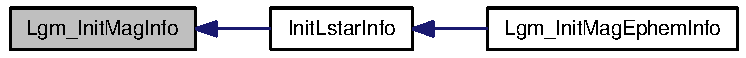
\includegraphics[width=197pt]{_lgm___mag_model_info_8h_4f16baeb21ae293220cd048d7bb8f757_icgraph}
\end{center}
\end{figure}
\hypertarget{_lgm___mag_model_info_8h_87ae57349dac55ae7393b6a168c080b2}{
\index{Lgm\_\-MagModelInfo.h@{Lgm\_\-MagModelInfo.h}!Lgm\_\-FreeMagInfo@{Lgm\_\-FreeMagInfo}}
\index{Lgm\_\-FreeMagInfo@{Lgm\_\-FreeMagInfo}!Lgm_MagModelInfo.h@{Lgm\_\-MagModelInfo.h}}
\subsubsection[{Lgm\_\-FreeMagInfo}]{\setlength{\rightskip}{0pt plus 5cm}void Lgm\_\-FreeMagInfo ({\bf Lgm\_\-MagModelInfo} $\ast$ {\em Info})}}
\label{_lgm___mag_model_info_8h_87ae57349dac55ae7393b6a168c080b2}




Definition at line 75 of file Lgm\_\-InitMagInfo.c.

Here is the call graph for this function:\nopagebreak
\begin{figure}[H]
\begin{center}
\leavevmode
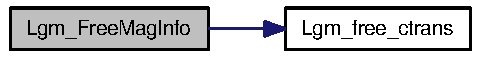
\includegraphics[width=133pt]{_lgm___mag_model_info_8h_87ae57349dac55ae7393b6a168c080b2_cgraph}
\end{center}
\end{figure}


Here is the caller graph for this function:\nopagebreak
\begin{figure}[H]
\begin{center}
\leavevmode
\includegraphics[width=206pt]{_lgm___mag_model_info_8h_87ae57349dac55ae7393b6a168c080b2_icgraph}
\end{center}
\end{figure}
\hypertarget{_lgm___mag_model_info_8h_d3b20a753c7c6d9afef944a6cf9880dc}{
\index{Lgm\_\-MagModelInfo.h@{Lgm\_\-MagModelInfo.h}!Lgm\_\-CopyMagInfo@{Lgm\_\-CopyMagInfo}}
\index{Lgm\_\-CopyMagInfo@{Lgm\_\-CopyMagInfo}!Lgm_MagModelInfo.h@{Lgm\_\-MagModelInfo.h}}
\subsubsection[{Lgm\_\-CopyMagInfo}]{\setlength{\rightskip}{0pt plus 5cm}{\bf Lgm\_\-MagModelInfo}$\ast$ Lgm\_\-CopyMagInfo ({\bf Lgm\_\-MagModelInfo} $\ast$ {\em s})}}
\label{_lgm___mag_model_info_8h_d3b20a753c7c6d9afef944a6cf9880dc}




Definition at line 90 of file Lgm\_\-InitMagInfo.c.

Here is the call graph for this function:\nopagebreak
\begin{figure}[H]
\begin{center}
\leavevmode
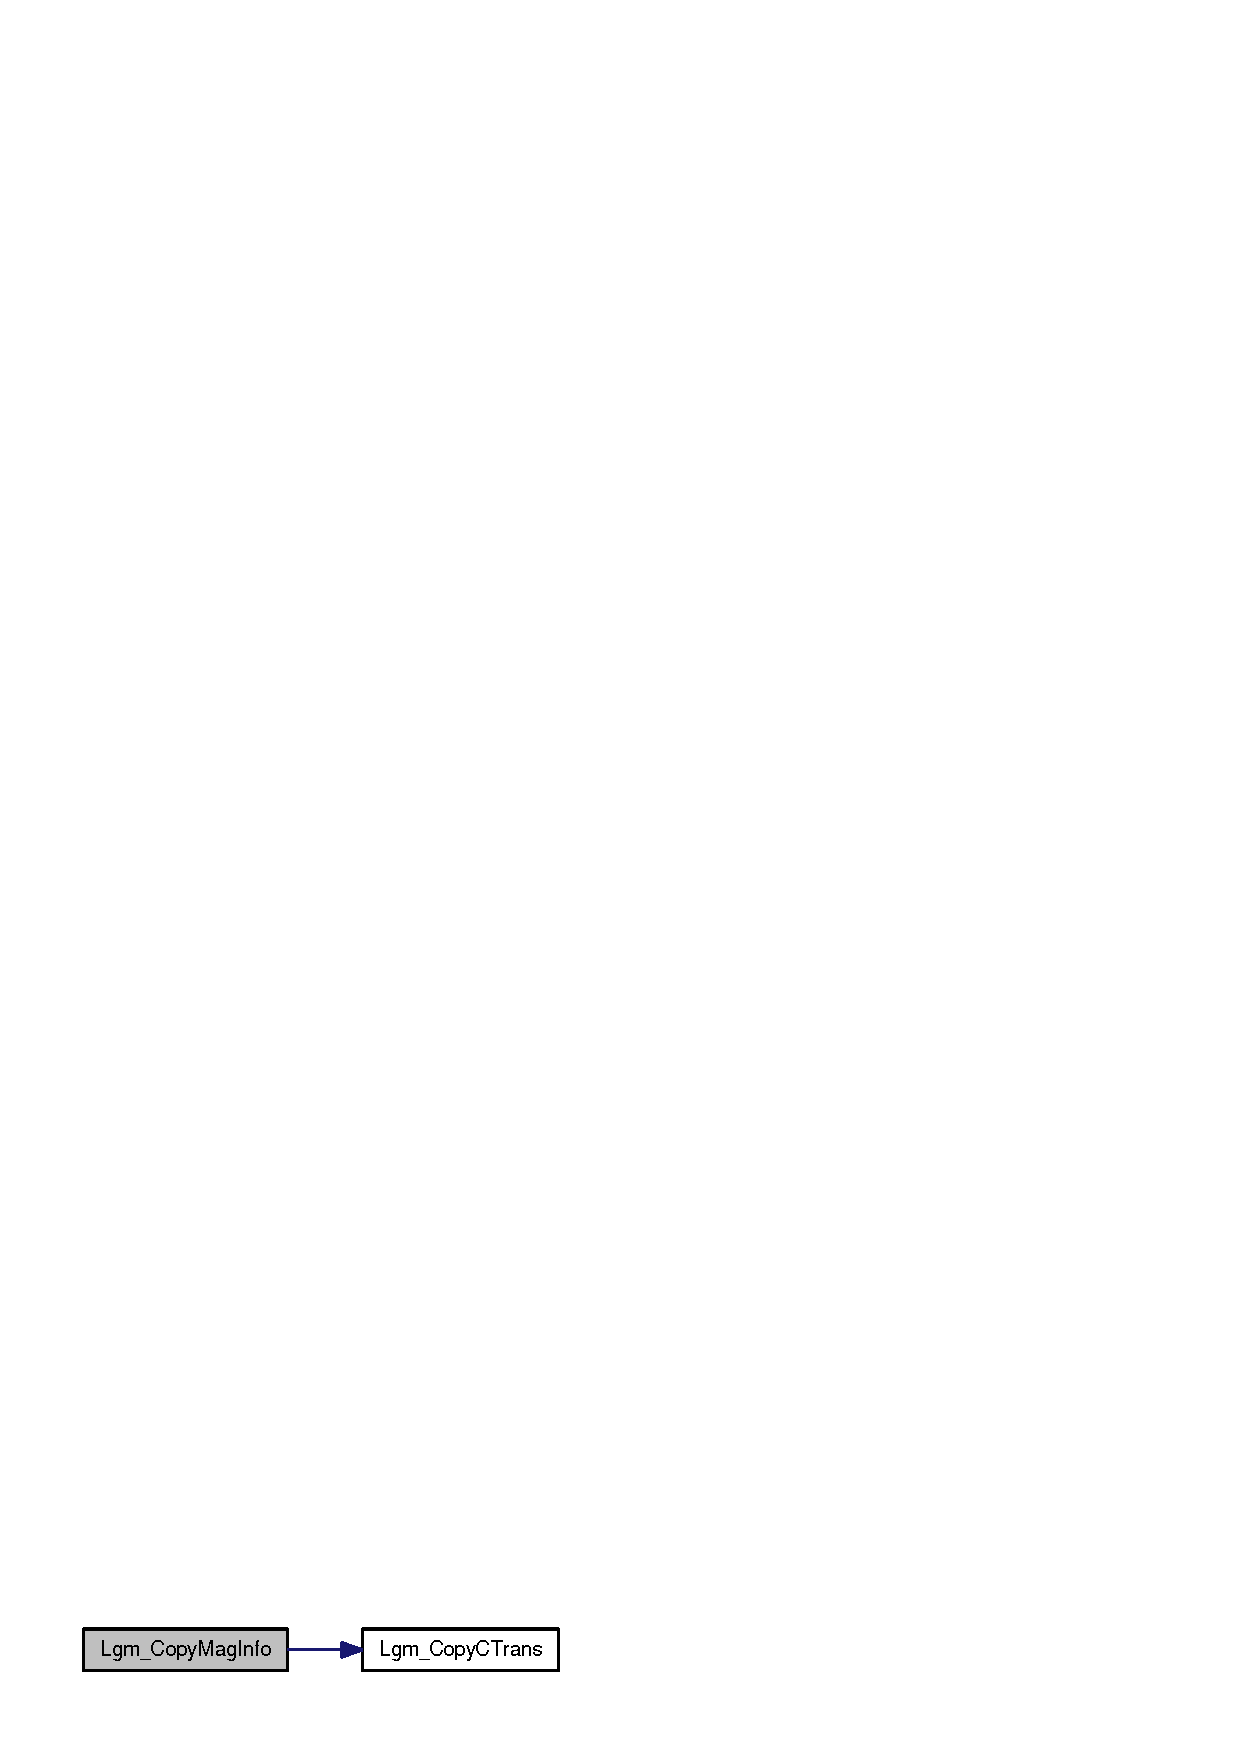
\includegraphics[width=136pt]{_lgm___mag_model_info_8h_d3b20a753c7c6d9afef944a6cf9880dc_cgraph}
\end{center}
\end{figure}


Here is the caller graph for this function:\nopagebreak
\begin{figure}[H]
\begin{center}
\leavevmode
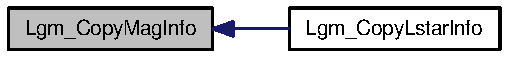
\includegraphics[width=140pt]{_lgm___mag_model_info_8h_d3b20a753c7c6d9afef944a6cf9880dc_icgraph}
\end{center}
\end{figure}
\hypertarget{_lgm___mag_model_info_8h_8a39a610942825fe168938aaddec20d7}{
\index{Lgm\_\-MagModelInfo.h@{Lgm\_\-MagModelInfo.h}!Lgm\_\-Trace@{Lgm\_\-Trace}}
\index{Lgm\_\-Trace@{Lgm\_\-Trace}!Lgm_MagModelInfo.h@{Lgm\_\-MagModelInfo.h}}
\subsubsection[{Lgm\_\-Trace}]{\setlength{\rightskip}{0pt plus 5cm}int Lgm\_\-Trace ({\bf Lgm\_\-Vector} $\ast$ {\em u}, \/  {\bf Lgm\_\-Vector} $\ast$ {\em v1}, \/  {\bf Lgm\_\-Vector} $\ast$ {\em v2}, \/  {\bf Lgm\_\-Vector} $\ast$ {\em v3}, \/  double {\em Height}, \/  double {\em TOL1}, \/  double {\em TOL2}, \/  {\bf Lgm\_\-MagModelInfo} $\ast$ {\em Info})}}
\label{_lgm___mag_model_info_8h_8a39a610942825fe168938aaddec20d7}




Definition at line 49 of file Lgm\_\-Trace.c.

Here is the call graph for this function:\nopagebreak
\begin{figure}[H]
\begin{center}
\leavevmode
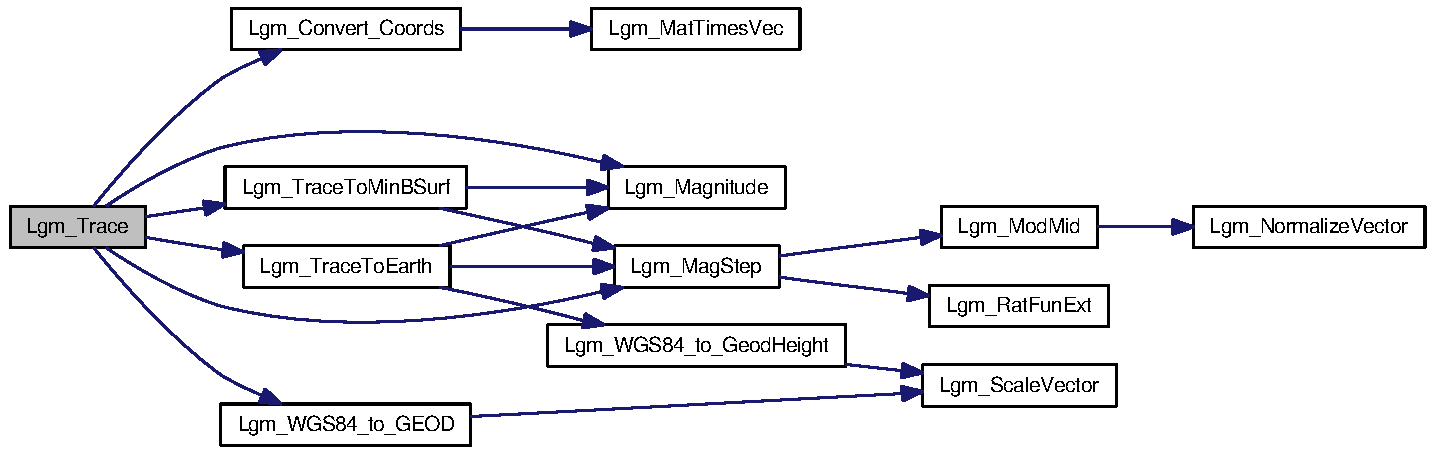
\includegraphics[width=362pt]{_lgm___mag_model_info_8h_8a39a610942825fe168938aaddec20d7_cgraph}
\end{center}
\end{figure}


Here is the caller graph for this function:\nopagebreak
\begin{figure}[H]
\begin{center}
\leavevmode
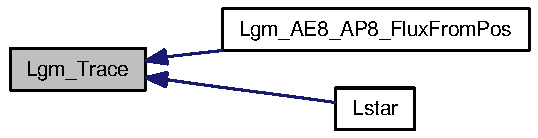
\includegraphics[width=147pt]{_lgm___mag_model_info_8h_8a39a610942825fe168938aaddec20d7_icgraph}
\end{center}
\end{figure}
\hypertarget{_lgm___mag_model_info_8h_e26694e4b9c3747fea07eadd0142142e}{
\index{Lgm\_\-MagModelInfo.h@{Lgm\_\-MagModelInfo.h}!Lgm\_\-TraceToMinBSurf@{Lgm\_\-TraceToMinBSurf}}
\index{Lgm\_\-TraceToMinBSurf@{Lgm\_\-TraceToMinBSurf}!Lgm_MagModelInfo.h@{Lgm\_\-MagModelInfo.h}}
\subsubsection[{Lgm\_\-TraceToMinBSurf}]{\setlength{\rightskip}{0pt plus 5cm}int Lgm\_\-TraceToMinBSurf ({\bf Lgm\_\-Vector} $\ast$, \/  {\bf Lgm\_\-Vector} $\ast$, \/  double, \/  double, \/  {\bf Lgm\_\-MagModelInfo} $\ast$)}}
\label{_lgm___mag_model_info_8h_e26694e4b9c3747fea07eadd0142142e}




Definition at line 21 of file TraceToMinBSurf.c.

Here is the call graph for this function:\nopagebreak
\begin{figure}[H]
\begin{center}
\leavevmode
\includegraphics[width=276pt]{_lgm___mag_model_info_8h_e26694e4b9c3747fea07eadd0142142e_cgraph}
\end{center}
\end{figure}


Here is the caller graph for this function:\nopagebreak
\begin{figure}[H]
\begin{center}
\leavevmode
\includegraphics[width=223pt]{_lgm___mag_model_info_8h_e26694e4b9c3747fea07eadd0142142e_icgraph}
\end{center}
\end{figure}
\hypertarget{_lgm___mag_model_info_8h_ae8951bf644962b97b86b6293e7c71c4}{
\index{Lgm\_\-MagModelInfo.h@{Lgm\_\-MagModelInfo.h}!Lgm\_\-TraceToSMEquat@{Lgm\_\-TraceToSMEquat}}
\index{Lgm\_\-TraceToSMEquat@{Lgm\_\-TraceToSMEquat}!Lgm_MagModelInfo.h@{Lgm\_\-MagModelInfo.h}}
\subsubsection[{Lgm\_\-TraceToSMEquat}]{\setlength{\rightskip}{0pt plus 5cm}int Lgm\_\-TraceToSMEquat ({\bf Lgm\_\-Vector} $\ast$, \/  {\bf Lgm\_\-Vector} $\ast$, \/  double, \/  {\bf Lgm\_\-MagModelInfo} $\ast$)}}
\label{_lgm___mag_model_info_8h_ae8951bf644962b97b86b6293e7c71c4}




Definition at line 23 of file TraceToSMEquat.c.

Here is the call graph for this function:\nopagebreak
\begin{figure}[H]
\begin{center}
\leavevmode
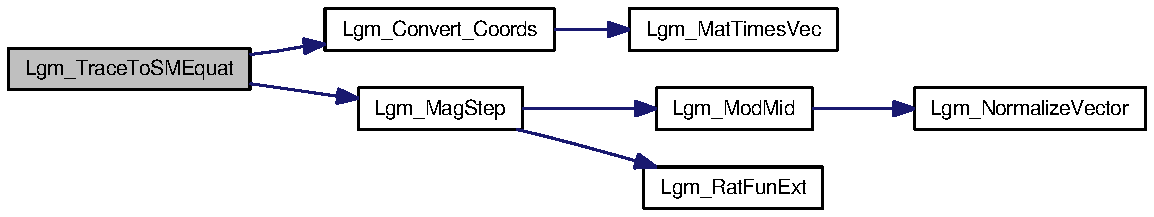
\includegraphics[width=295pt]{_lgm___mag_model_info_8h_ae8951bf644962b97b86b6293e7c71c4_cgraph}
\end{center}
\end{figure}
\hypertarget{_lgm___mag_model_info_8h_7b45a70ceb729d0b1f485e8aa67bd24f}{
\index{Lgm\_\-MagModelInfo.h@{Lgm\_\-MagModelInfo.h}!Lgm\_\-TraceToEarth@{Lgm\_\-TraceToEarth}}
\index{Lgm\_\-TraceToEarth@{Lgm\_\-TraceToEarth}!Lgm_MagModelInfo.h@{Lgm\_\-MagModelInfo.h}}
\subsubsection[{Lgm\_\-TraceToEarth}]{\setlength{\rightskip}{0pt plus 5cm}int Lgm\_\-TraceToEarth ({\bf Lgm\_\-Vector} $\ast$, \/  {\bf Lgm\_\-Vector} $\ast$, \/  double, \/  double, \/  double, \/  {\bf Lgm\_\-MagModelInfo} $\ast$)}}
\label{_lgm___mag_model_info_8h_7b45a70ceb729d0b1f485e8aa67bd24f}




Definition at line 25 of file Lgm\_\-TraceToEarth.c.

Here is the call graph for this function:\nopagebreak
\begin{figure}[H]
\begin{center}
\leavevmode
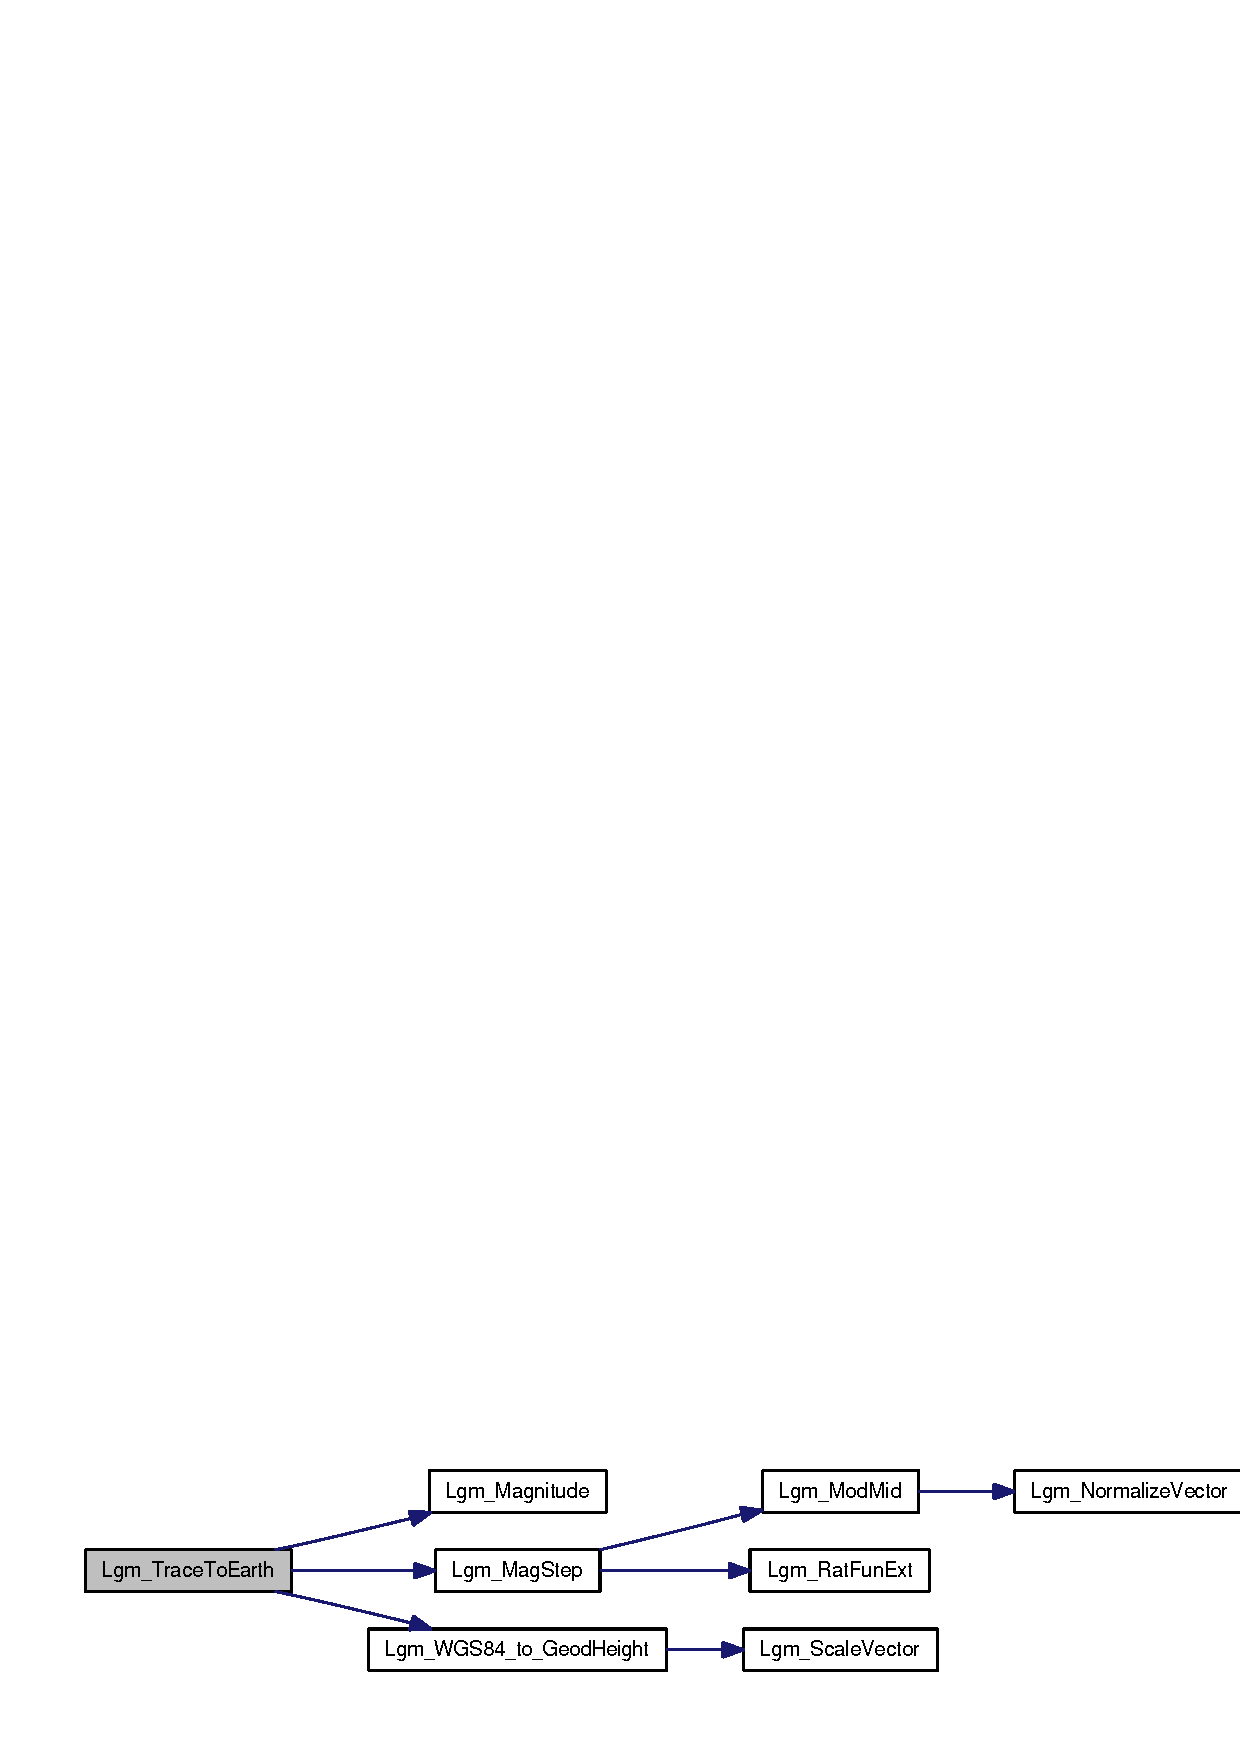
\includegraphics[width=301pt]{_lgm___mag_model_info_8h_7b45a70ceb729d0b1f485e8aa67bd24f_cgraph}
\end{center}
\end{figure}


Here is the caller graph for this function:\nopagebreak
\begin{figure}[H]
\begin{center}
\leavevmode
\includegraphics[width=215pt]{_lgm___mag_model_info_8h_7b45a70ceb729d0b1f485e8aa67bd24f_icgraph}
\end{center}
\end{figure}
\hypertarget{_lgm___mag_model_info_8h_b4590c6952725d09b17c1433371db4e2}{
\index{Lgm\_\-MagModelInfo.h@{Lgm\_\-MagModelInfo.h}!Lgm\_\-TraceToSphericalEarth@{Lgm\_\-TraceToSphericalEarth}}
\index{Lgm\_\-TraceToSphericalEarth@{Lgm\_\-TraceToSphericalEarth}!Lgm_MagModelInfo.h@{Lgm\_\-MagModelInfo.h}}
\subsubsection[{Lgm\_\-TraceToSphericalEarth}]{\setlength{\rightskip}{0pt plus 5cm}int Lgm\_\-TraceToSphericalEarth ({\bf Lgm\_\-Vector} $\ast$, \/  {\bf Lgm\_\-Vector} $\ast$, \/  double, \/  double, \/  double, \/  {\bf Lgm\_\-MagModelInfo} $\ast$)}}
\label{_lgm___mag_model_info_8h_b4590c6952725d09b17c1433371db4e2}




Definition at line 32 of file Lgm\_\-TraceToSphericalEarth.c.

Here is the call graph for this function:\nopagebreak
\begin{figure}[H]
\begin{center}
\leavevmode
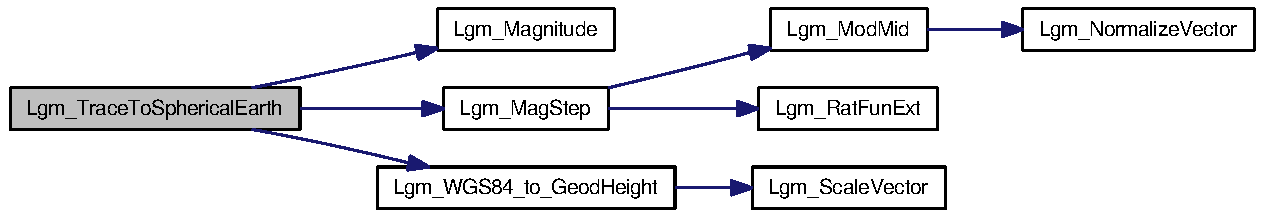
\includegraphics[width=321pt]{_lgm___mag_model_info_8h_b4590c6952725d09b17c1433371db4e2_cgraph}
\end{center}
\end{figure}


Here is the caller graph for this function:\nopagebreak
\begin{figure}[H]
\begin{center}
\leavevmode
\includegraphics[width=129pt]{_lgm___mag_model_info_8h_b4590c6952725d09b17c1433371db4e2_icgraph}
\end{center}
\end{figure}
\hypertarget{_lgm___mag_model_info_8h_68681484778e87dde0f6f80a8fee549f}{
\index{Lgm\_\-MagModelInfo.h@{Lgm\_\-MagModelInfo.h}!Lgm\_\-TraceLine@{Lgm\_\-TraceLine}}
\index{Lgm\_\-TraceLine@{Lgm\_\-TraceLine}!Lgm_MagModelInfo.h@{Lgm\_\-MagModelInfo.h}}
\subsubsection[{Lgm\_\-TraceLine}]{\setlength{\rightskip}{0pt plus 5cm}int Lgm\_\-TraceLine ({\bf Lgm\_\-Vector} $\ast$, \/  {\bf Lgm\_\-Vector} $\ast$, \/  double, \/  double, \/  double, \/  int, \/  {\bf Lgm\_\-MagModelInfo} $\ast$)}}
\label{_lgm___mag_model_info_8h_68681484778e87dde0f6f80a8fee549f}




Definition at line 55 of file TraceLine.c.

Here is the call graph for this function:\nopagebreak
\begin{figure}[H]
\begin{center}
\leavevmode
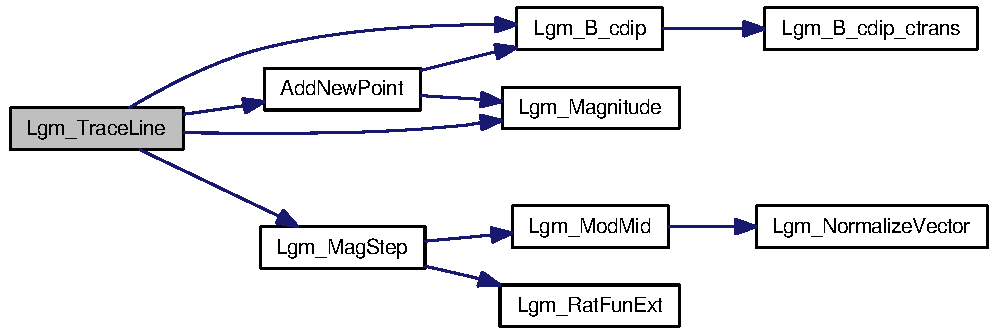
\includegraphics[width=257pt]{_lgm___mag_model_info_8h_68681484778e87dde0f6f80a8fee549f_cgraph}
\end{center}
\end{figure}


Here is the caller graph for this function:\nopagebreak
\begin{figure}[H]
\begin{center}
\leavevmode
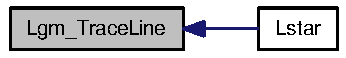
\includegraphics[width=101pt]{_lgm___mag_model_info_8h_68681484778e87dde0f6f80a8fee549f_icgraph}
\end{center}
\end{figure}
\hypertarget{_lgm___mag_model_info_8h_97c791c85beb7f0f5f816f79226b2e2c}{
\index{Lgm\_\-MagModelInfo.h@{Lgm\_\-MagModelInfo.h}!Lgm\_\-TraceLine2@{Lgm\_\-TraceLine2}}
\index{Lgm\_\-TraceLine2@{Lgm\_\-TraceLine2}!Lgm_MagModelInfo.h@{Lgm\_\-MagModelInfo.h}}
\subsubsection[{Lgm\_\-TraceLine2}]{\setlength{\rightskip}{0pt plus 5cm}int Lgm\_\-TraceLine2 ({\bf Lgm\_\-Vector} $\ast$, \/  {\bf Lgm\_\-Vector} $\ast$, \/  double, \/  double, \/  double, \/  double, \/  int, \/  {\bf Lgm\_\-MagModelInfo} $\ast$)}}
\label{_lgm___mag_model_info_8h_97c791c85beb7f0f5f816f79226b2e2c}




Definition at line 340 of file TraceLine.c.

Here is the call graph for this function:\nopagebreak
\begin{figure}[H]
\begin{center}
\leavevmode
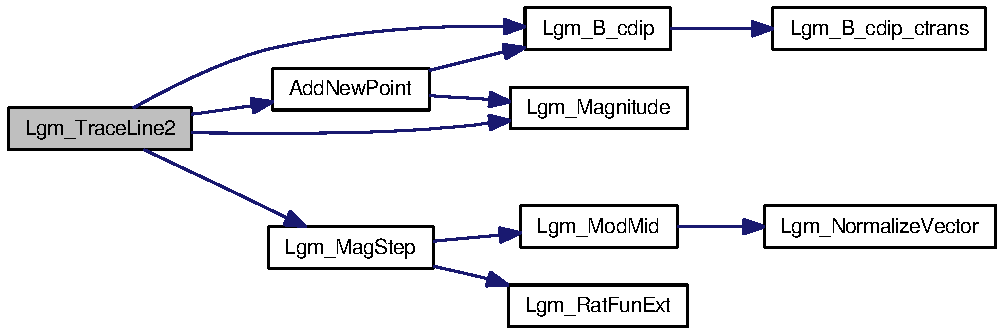
\includegraphics[width=259pt]{_lgm___mag_model_info_8h_97c791c85beb7f0f5f816f79226b2e2c_cgraph}
\end{center}
\end{figure}


Here is the caller graph for this function:\nopagebreak
\begin{figure}[H]
\begin{center}
\leavevmode
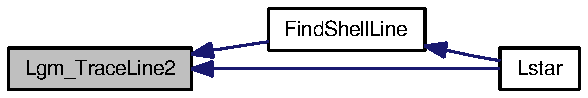
\includegraphics[width=159pt]{_lgm___mag_model_info_8h_97c791c85beb7f0f5f816f79226b2e2c_icgraph}
\end{center}
\end{figure}
\hypertarget{_lgm___mag_model_info_8h_069290bbefbad1db8e625b9e8a0d3a5e}{
\index{Lgm\_\-MagModelInfo.h@{Lgm\_\-MagModelInfo.h}!ReplaceFirstPoint@{ReplaceFirstPoint}}
\index{ReplaceFirstPoint@{ReplaceFirstPoint}!Lgm_MagModelInfo.h@{Lgm\_\-MagModelInfo.h}}
\subsubsection[{ReplaceFirstPoint}]{\setlength{\rightskip}{0pt plus 5cm}void ReplaceFirstPoint (double {\em s}, \/  double {\em B}, \/  {\bf Lgm\_\-Vector} $\ast$ {\em P}, \/  {\bf Lgm\_\-MagModelInfo} $\ast$ {\em Info})}}
\label{_lgm___mag_model_info_8h_069290bbefbad1db8e625b9e8a0d3a5e}




Definition at line 580 of file TraceLine.c.

Here is the call graph for this function:\nopagebreak
\begin{figure}[H]
\begin{center}
\leavevmode
\includegraphics[width=199pt]{_lgm___mag_model_info_8h_069290bbefbad1db8e625b9e8a0d3a5e_cgraph}
\end{center}
\end{figure}


Here is the caller graph for this function:\nopagebreak
\begin{figure}[H]
\begin{center}
\leavevmode
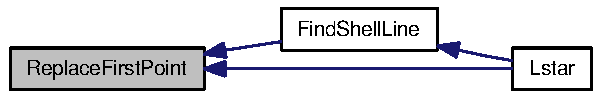
\includegraphics[width=162pt]{_lgm___mag_model_info_8h_069290bbefbad1db8e625b9e8a0d3a5e_icgraph}
\end{center}
\end{figure}
\hypertarget{_lgm___mag_model_info_8h_a82612dffc3edae2b3fce7cb94e435c0}{
\index{Lgm\_\-MagModelInfo.h@{Lgm\_\-MagModelInfo.h}!AddNewPoint@{AddNewPoint}}
\index{AddNewPoint@{AddNewPoint}!Lgm_MagModelInfo.h@{Lgm\_\-MagModelInfo.h}}
\subsubsection[{AddNewPoint}]{\setlength{\rightskip}{0pt plus 5cm}void AddNewPoint (double {\em s}, \/  double {\em B}, \/  {\bf Lgm\_\-Vector} $\ast$ {\em P}, \/  {\bf Lgm\_\-MagModelInfo} $\ast$ {\em Info})}}
\label{_lgm___mag_model_info_8h_a82612dffc3edae2b3fce7cb94e435c0}




Definition at line 595 of file TraceLine.c.

Here is the call graph for this function:\nopagebreak
\begin{figure}[H]
\begin{center}
\leavevmode
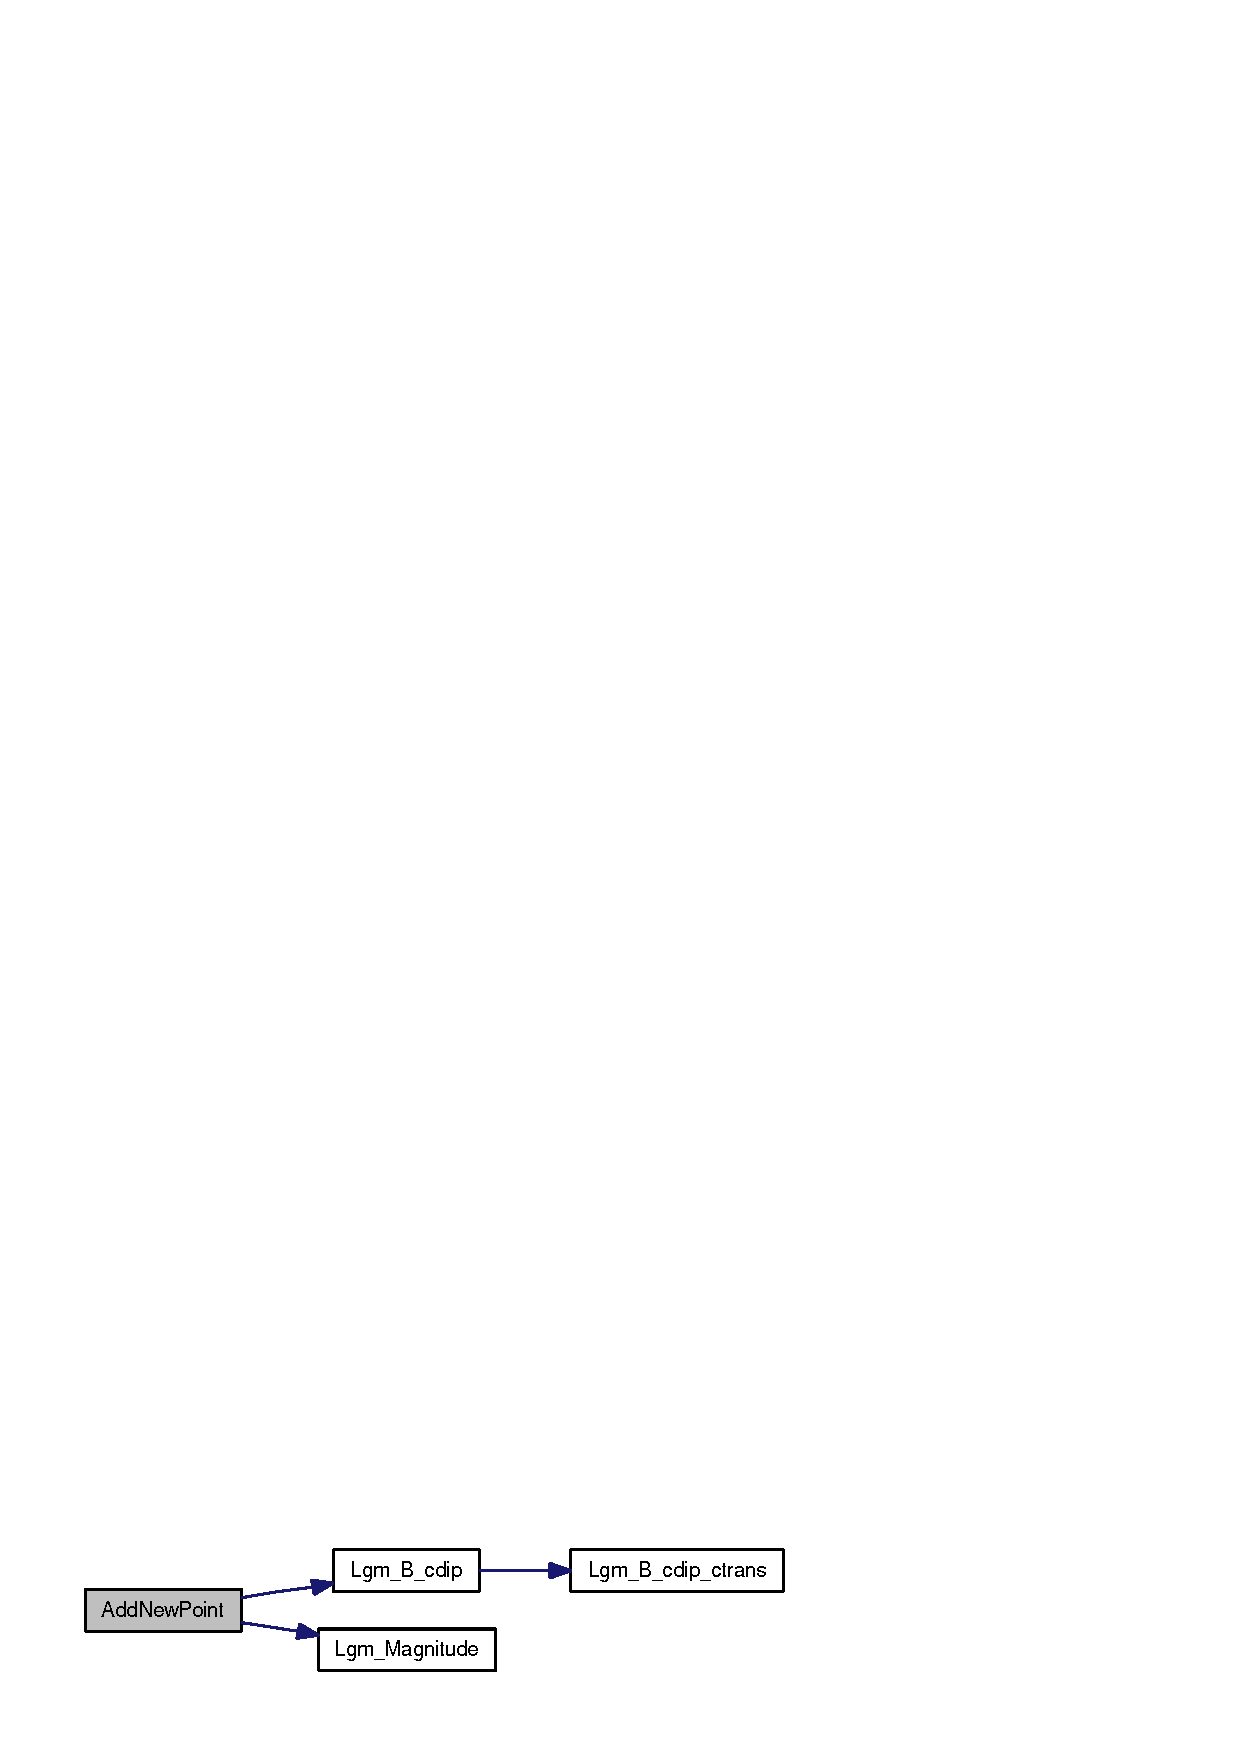
\includegraphics[width=190pt]{_lgm___mag_model_info_8h_a82612dffc3edae2b3fce7cb94e435c0_cgraph}
\end{center}
\end{figure}


Here is the caller graph for this function:\nopagebreak
\begin{figure}[H]
\begin{center}
\leavevmode
\includegraphics[width=219pt]{_lgm___mag_model_info_8h_a82612dffc3edae2b3fce7cb94e435c0_icgraph}
\end{center}
\end{figure}
\hypertarget{_lgm___mag_model_info_8h_a7175b98aed0d6f712ca66d532afe450}{
\index{Lgm\_\-MagModelInfo.h@{Lgm\_\-MagModelInfo.h}!InitSpline@{InitSpline}}
\index{InitSpline@{InitSpline}!Lgm_MagModelInfo.h@{Lgm\_\-MagModelInfo.h}}
\subsubsection[{InitSpline}]{\setlength{\rightskip}{0pt plus 5cm}void InitSpline ({\bf Lgm\_\-MagModelInfo} $\ast$ {\em Info})}}
\label{_lgm___mag_model_info_8h_a7175b98aed0d6f712ca66d532afe450}




Definition at line 667 of file TraceLine.c.

Here is the caller graph for this function:\nopagebreak
\begin{figure}[H]
\begin{center}
\leavevmode
\includegraphics[width=154pt]{_lgm___mag_model_info_8h_a7175b98aed0d6f712ca66d532afe450_icgraph}
\end{center}
\end{figure}
\hypertarget{_lgm___mag_model_info_8h_e748e444fc7e684dcead584e1d002e8d}{
\index{Lgm\_\-MagModelInfo.h@{Lgm\_\-MagModelInfo.h}!FreeSpline@{FreeSpline}}
\index{FreeSpline@{FreeSpline}!Lgm_MagModelInfo.h@{Lgm\_\-MagModelInfo.h}}
\subsubsection[{FreeSpline}]{\setlength{\rightskip}{0pt plus 5cm}void FreeSpline ({\bf Lgm\_\-MagModelInfo} $\ast$ {\em Info})}}
\label{_lgm___mag_model_info_8h_e748e444fc7e684dcead584e1d002e8d}




Definition at line 716 of file TraceLine.c.

Here is the caller graph for this function:\nopagebreak
\begin{figure}[H]
\begin{center}
\leavevmode
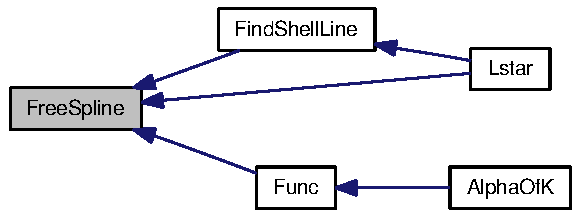
\includegraphics[width=157pt]{_lgm___mag_model_info_8h_e748e444fc7e684dcead584e1d002e8d_icgraph}
\end{center}
\end{figure}
\hypertarget{_lgm___mag_model_info_8h_c00bd91234cdbfb21a2fdf225f257668}{
\index{Lgm\_\-MagModelInfo.h@{Lgm\_\-MagModelInfo.h}!Lgm\_\-TraceToMinRdotB@{Lgm\_\-TraceToMinRdotB}}
\index{Lgm\_\-TraceToMinRdotB@{Lgm\_\-TraceToMinRdotB}!Lgm_MagModelInfo.h@{Lgm\_\-MagModelInfo.h}}
\subsubsection[{Lgm\_\-TraceToMinRdotB}]{\setlength{\rightskip}{0pt plus 5cm}int Lgm\_\-TraceToMinRdotB ({\bf Lgm\_\-Vector} $\ast$, \/  {\bf Lgm\_\-Vector} $\ast$, \/  double, \/  {\bf Lgm\_\-MagModelInfo} $\ast$)}}
\label{_lgm___mag_model_info_8h_c00bd91234cdbfb21a2fdf225f257668}




Definition at line 21 of file TraceToMinRdotB.c.

Here is the call graph for this function:\nopagebreak
\begin{figure}[H]
\begin{center}
\leavevmode
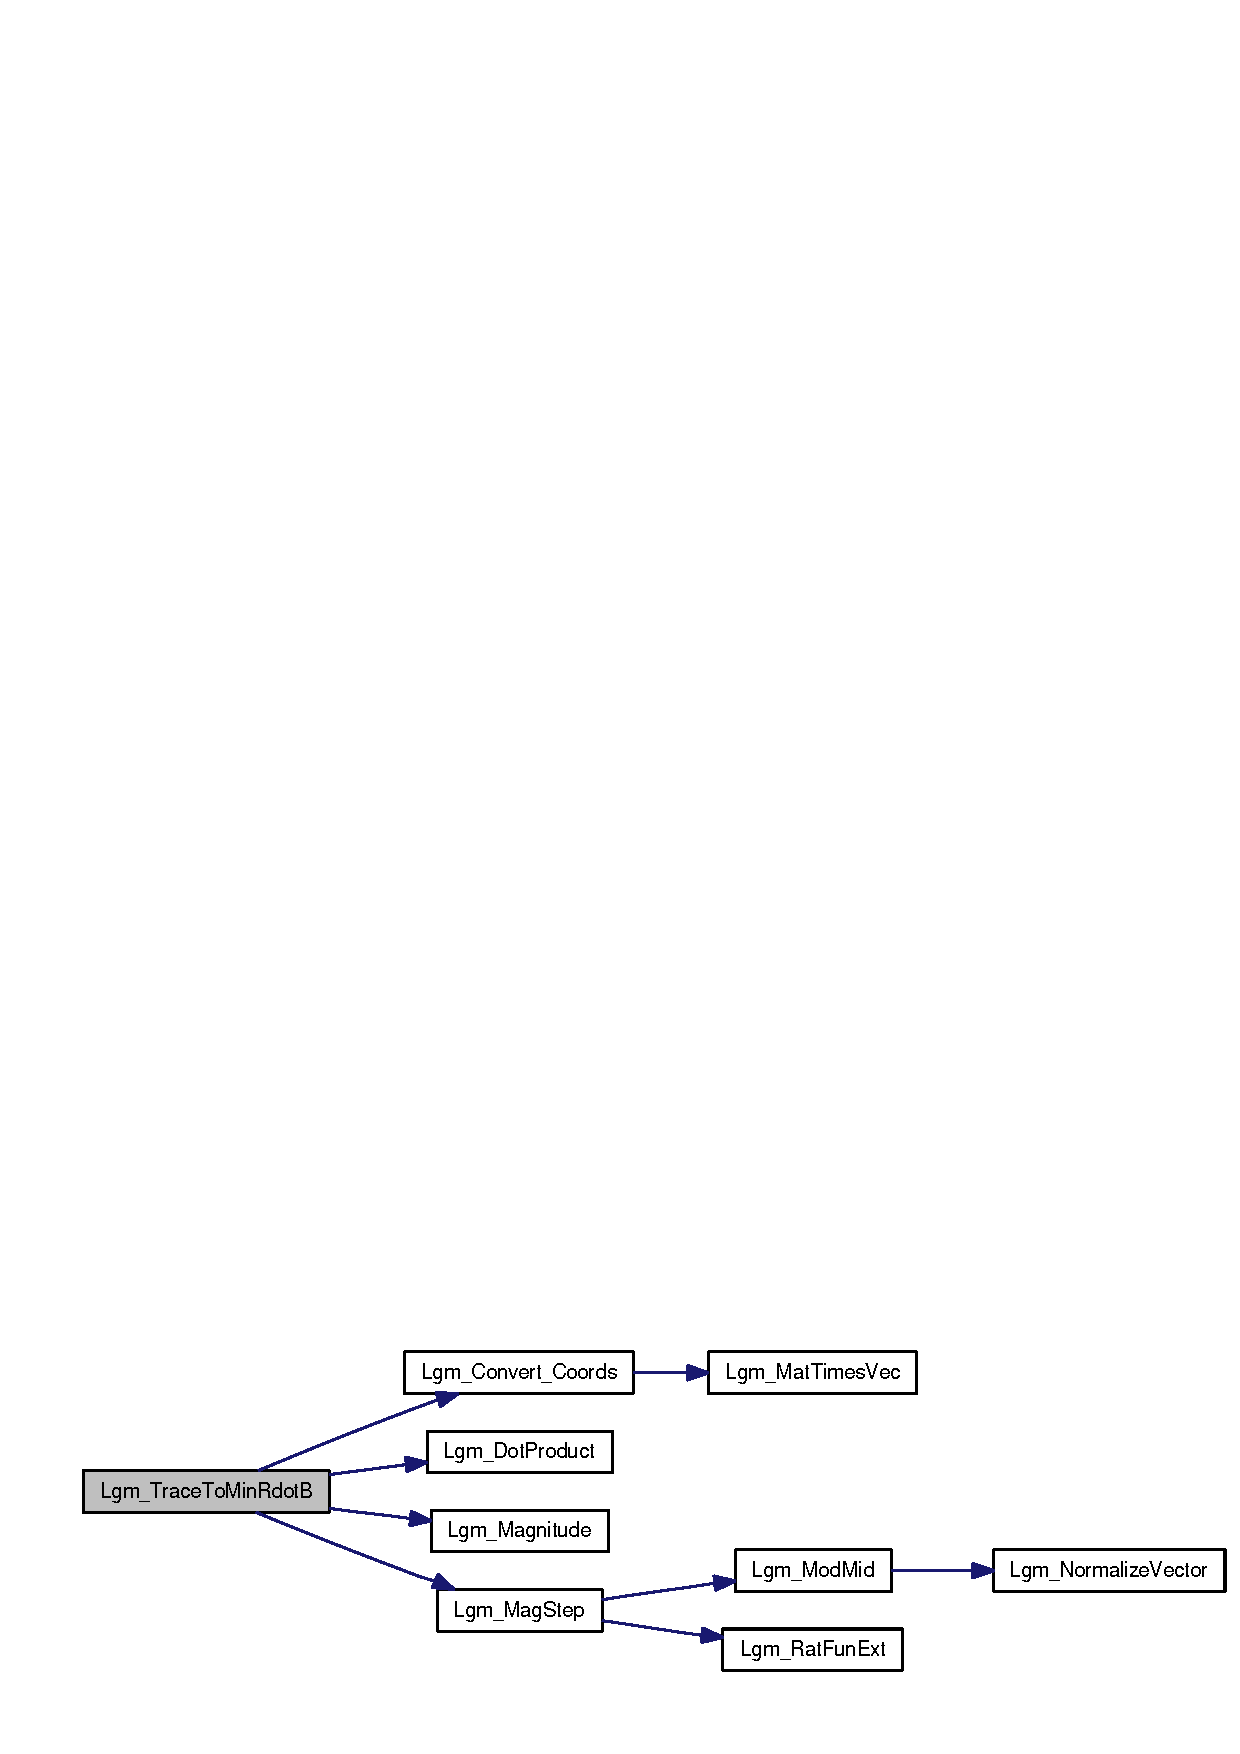
\includegraphics[width=296pt]{_lgm___mag_model_info_8h_c00bd91234cdbfb21a2fdf225f257668_cgraph}
\end{center}
\end{figure}
\hypertarget{_lgm___mag_model_info_8h_c4c1efecd6b1db18ee51b1b28cfe82db}{
\index{Lgm\_\-MagModelInfo.h@{Lgm\_\-MagModelInfo.h}!Lgm\_\-TraceIDL@{Lgm\_\-TraceIDL}}
\index{Lgm\_\-TraceIDL@{Lgm\_\-TraceIDL}!Lgm_MagModelInfo.h@{Lgm\_\-MagModelInfo.h}}
\subsubsection[{Lgm\_\-TraceIDL}]{\setlength{\rightskip}{0pt plus 5cm}int Lgm\_\-TraceIDL (int, \/  void $\ast$ {\em argv}\mbox{[}$\,$\mbox{]})}}
\label{_lgm___mag_model_info_8h_c4c1efecd6b1db18ee51b1b28cfe82db}


\hypertarget{_lgm___mag_model_info_8h_f5875fcc683e532736574a4edf7e8545}{
\index{Lgm\_\-MagModelInfo.h@{Lgm\_\-MagModelInfo.h}!Lgm\_\-TraceToMirrorPoint@{Lgm\_\-TraceToMirrorPoint}}
\index{Lgm\_\-TraceToMirrorPoint@{Lgm\_\-TraceToMirrorPoint}!Lgm_MagModelInfo.h@{Lgm\_\-MagModelInfo.h}}
\subsubsection[{Lgm\_\-TraceToMirrorPoint}]{\setlength{\rightskip}{0pt plus 5cm}int Lgm\_\-TraceToMirrorPoint ({\bf Lgm\_\-Vector} $\ast$ {\em u}, \/  {\bf Lgm\_\-Vector} $\ast$ {\em v}, \/  double $\ast$ {\em Sm}, \/  double {\em H0}, \/  double {\em Bm}, \/  double {\em sgn}, \/  double {\em tol}, \/  {\bf Lgm\_\-MagModelInfo} $\ast$ {\em Info})}}
\label{_lgm___mag_model_info_8h_f5875fcc683e532736574a4edf7e8545}




Definition at line 25 of file TraceToMirrorPoint2.c.

Here is the call graph for this function:\nopagebreak
\begin{figure}[H]
\begin{center}
\leavevmode
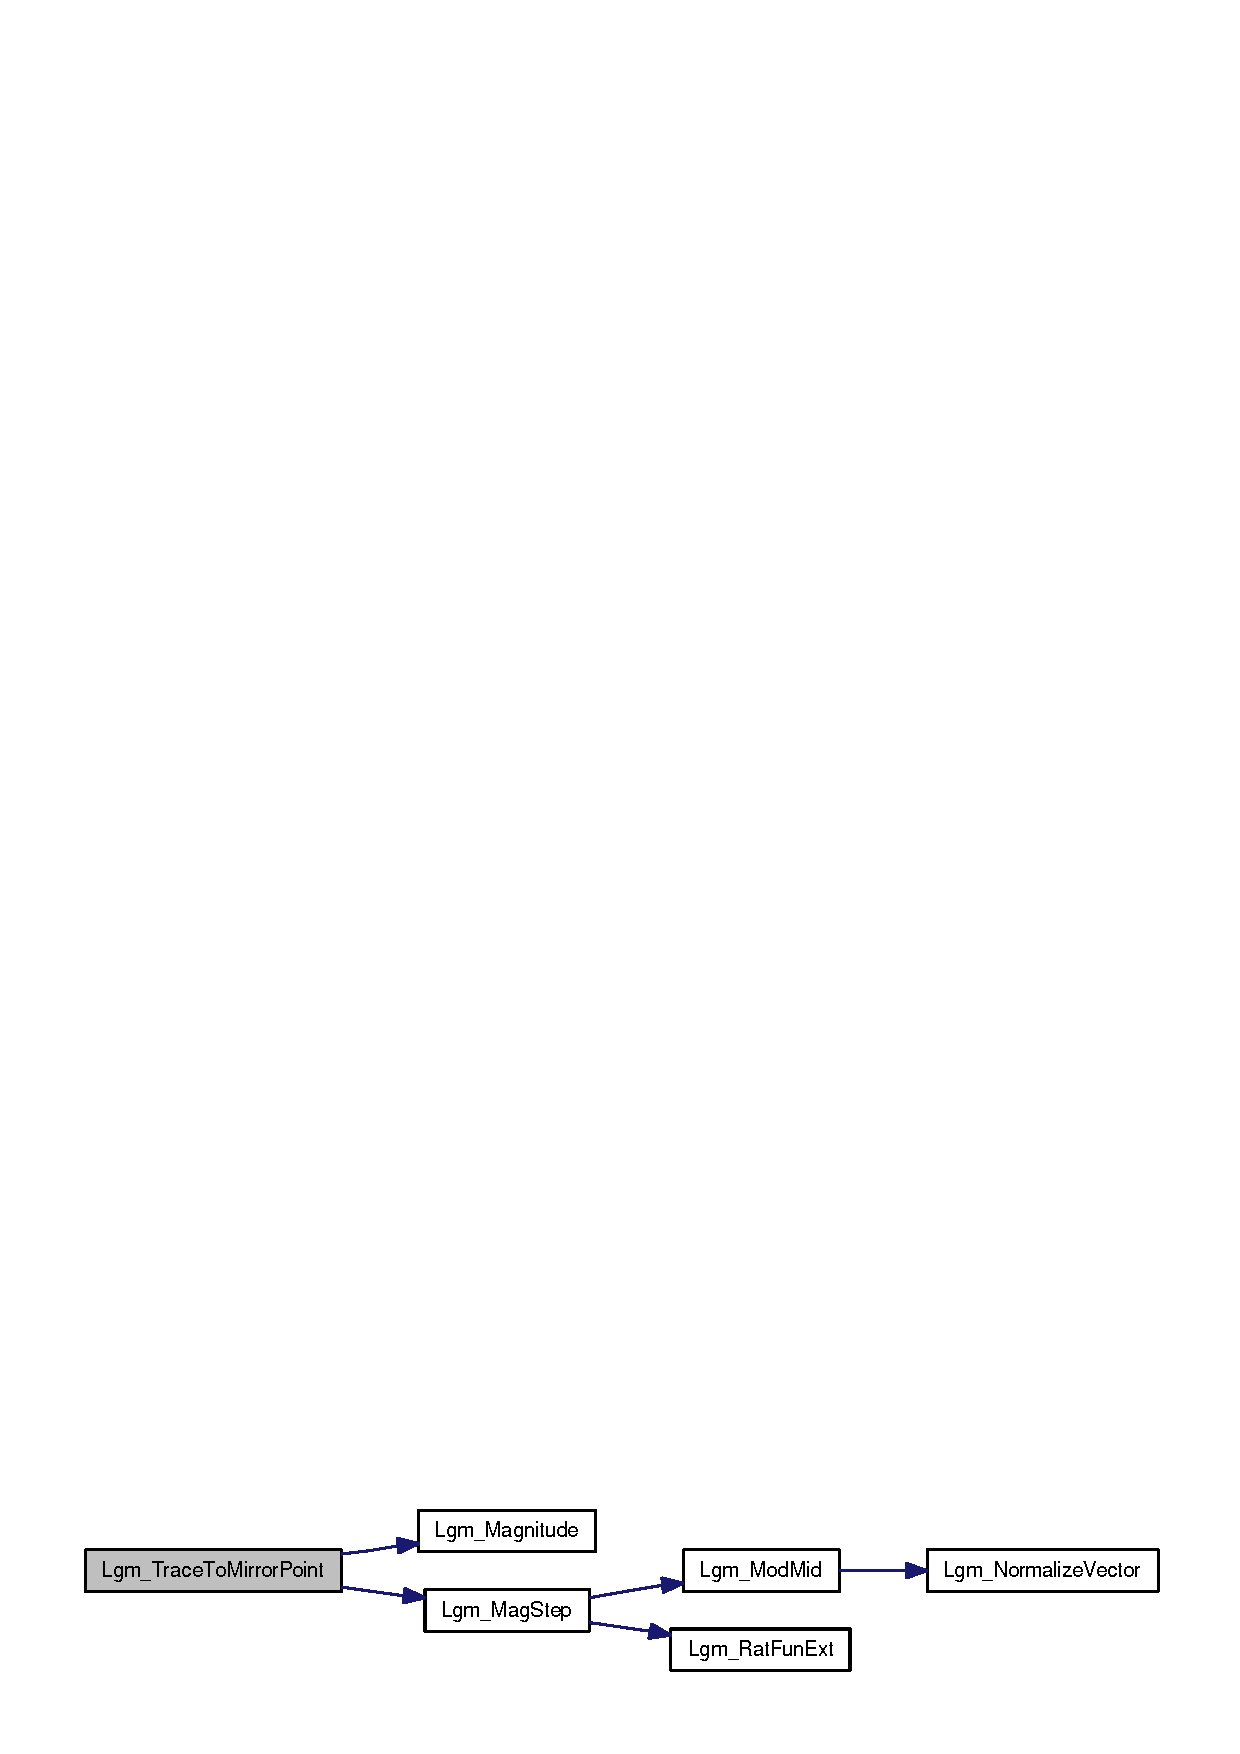
\includegraphics[width=280pt]{_lgm___mag_model_info_8h_f5875fcc683e532736574a4edf7e8545_cgraph}
\end{center}
\end{figure}


Here is the caller graph for this function:\nopagebreak
\begin{figure}[H]
\begin{center}
\leavevmode
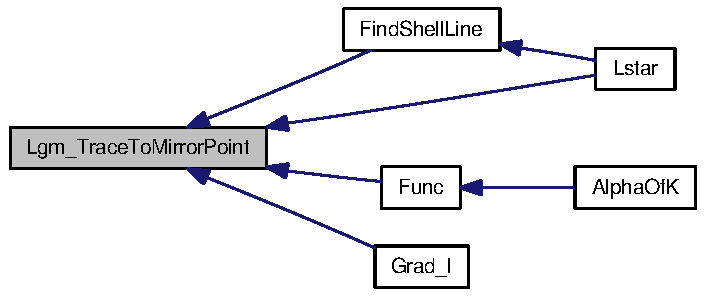
\includegraphics[width=187pt]{_lgm___mag_model_info_8h_f5875fcc683e532736574a4edf7e8545_icgraph}
\end{center}
\end{figure}
\hypertarget{_lgm___mag_model_info_8h_24e31c1882021ee661d8afd00d72e726}{
\index{Lgm\_\-MagModelInfo.h@{Lgm\_\-MagModelInfo.h}!Lgm\_\-ModMid@{Lgm\_\-ModMid}}
\index{Lgm\_\-ModMid@{Lgm\_\-ModMid}!Lgm_MagModelInfo.h@{Lgm\_\-MagModelInfo.h}}
\subsubsection[{Lgm\_\-ModMid}]{\setlength{\rightskip}{0pt plus 5cm}void Lgm\_\-ModMid ({\bf Lgm\_\-Vector} $\ast$, \/  {\bf Lgm\_\-Vector} $\ast$, \/  double, \/  int, \/  double, \/  int($\ast$)({\bf Lgm\_\-Vector} $\ast$, {\bf Lgm\_\-Vector} $\ast$, {\bf Lgm\_\-MagModelInfo} $\ast$) {\em Mag}, \/  {\bf Lgm\_\-MagModelInfo} $\ast$)}}
\label{_lgm___mag_model_info_8h_24e31c1882021ee661d8afd00d72e726}




Definition at line 17 of file MagStep.c.

Here is the call graph for this function:\nopagebreak
\begin{figure}[H]
\begin{center}
\leavevmode
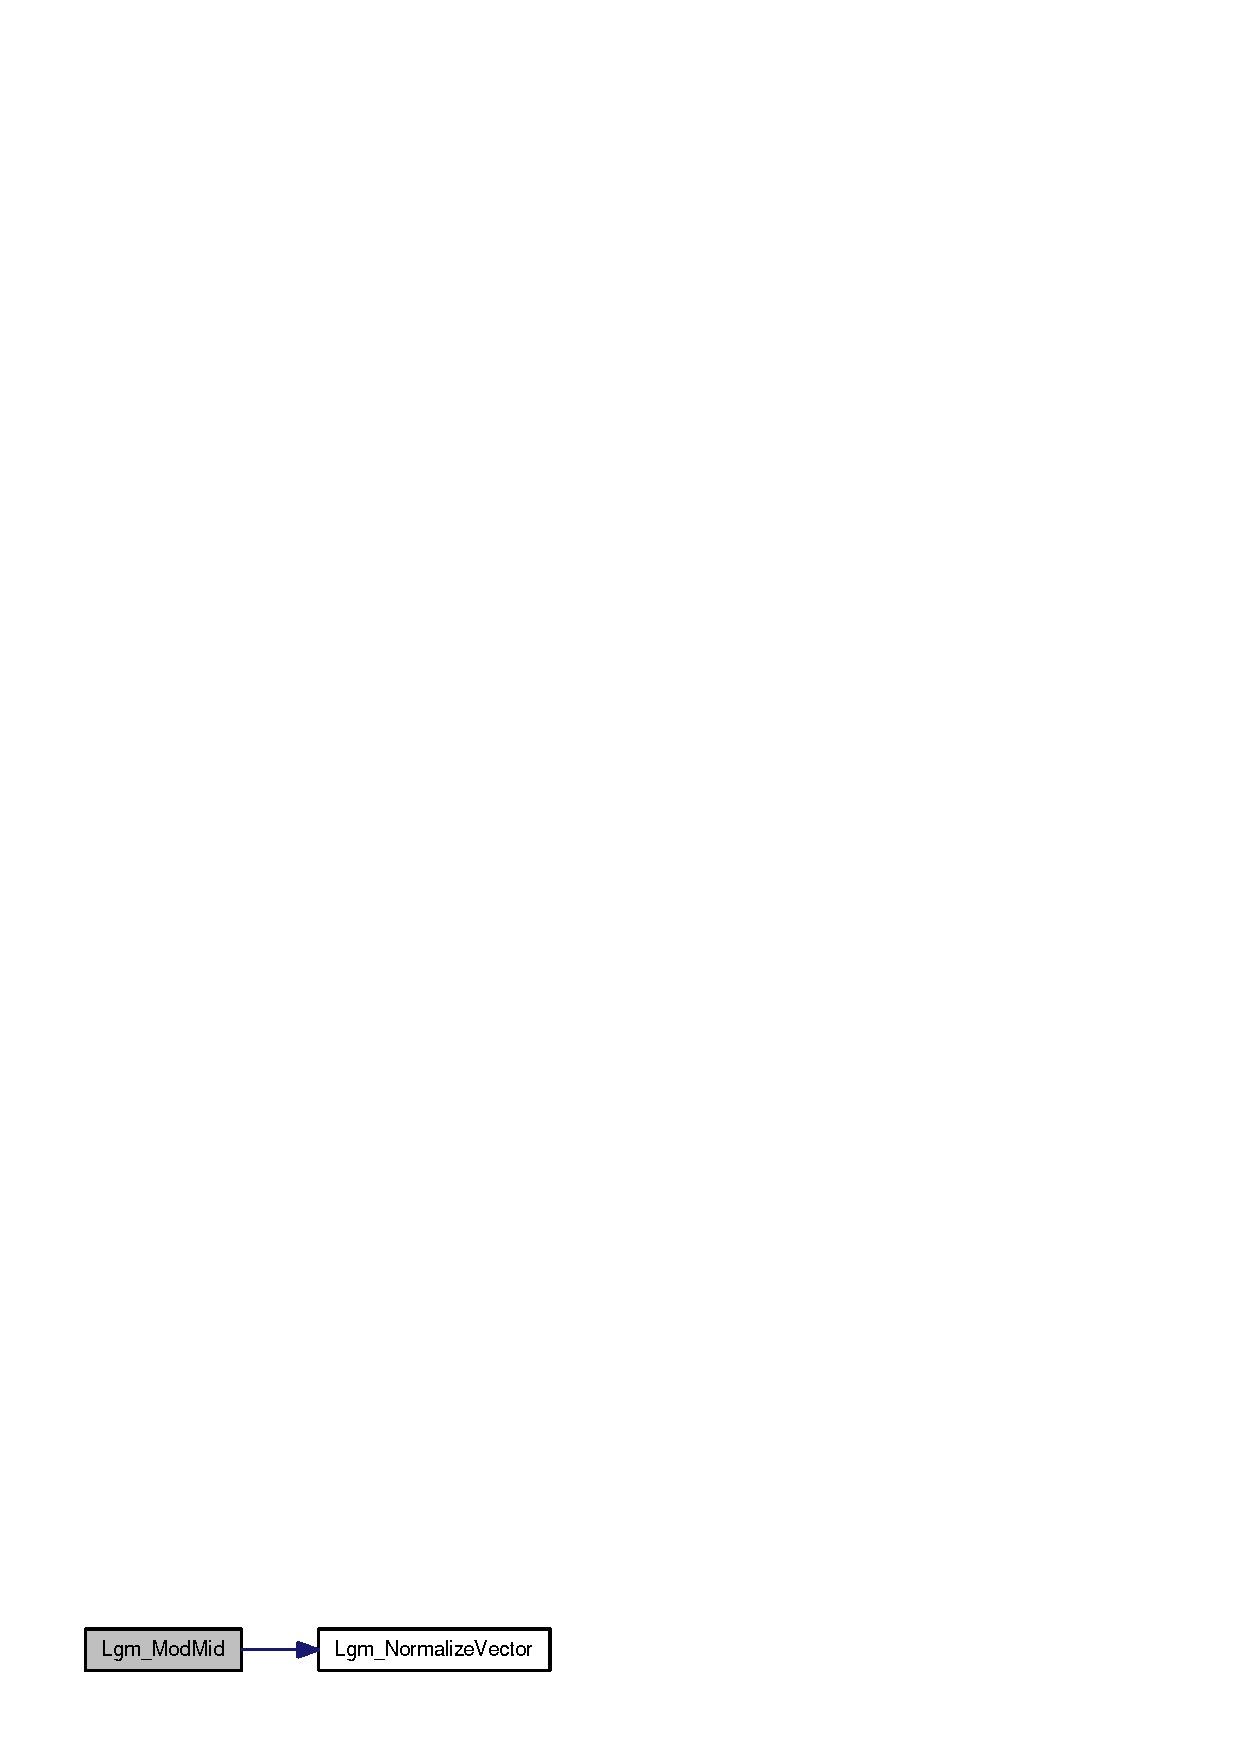
\includegraphics[width=134pt]{_lgm___mag_model_info_8h_24e31c1882021ee661d8afd00d72e726_cgraph}
\end{center}
\end{figure}


Here is the caller graph for this function:\nopagebreak
\begin{figure}[H]
\begin{center}
\leavevmode
\includegraphics[width=420pt]{_lgm___mag_model_info_8h_24e31c1882021ee661d8afd00d72e726_icgraph}
\end{center}
\end{figure}
\hypertarget{_lgm___mag_model_info_8h_1e8a22ce5672e4a4b9a51ca51713408e}{
\index{Lgm\_\-MagModelInfo.h@{Lgm\_\-MagModelInfo.h}!Lgm\_\-RatFunExt@{Lgm\_\-RatFunExt}}
\index{Lgm\_\-RatFunExt@{Lgm\_\-RatFunExt}!Lgm_MagModelInfo.h@{Lgm\_\-MagModelInfo.h}}
\subsubsection[{Lgm\_\-RatFunExt}]{\setlength{\rightskip}{0pt plus 5cm}void Lgm\_\-RatFunExt (int, \/  double, \/  {\bf Lgm\_\-Vector} $\ast$, \/  {\bf Lgm\_\-Vector} $\ast$, \/  {\bf Lgm\_\-Vector} $\ast$, \/  {\bf Lgm\_\-MagModelInfo} $\ast$)}}
\label{_lgm___mag_model_info_8h_1e8a22ce5672e4a4b9a51ca51713408e}




Definition at line 85 of file MagStep.c.

Here is the caller graph for this function:\nopagebreak
\begin{figure}[H]
\begin{center}
\leavevmode
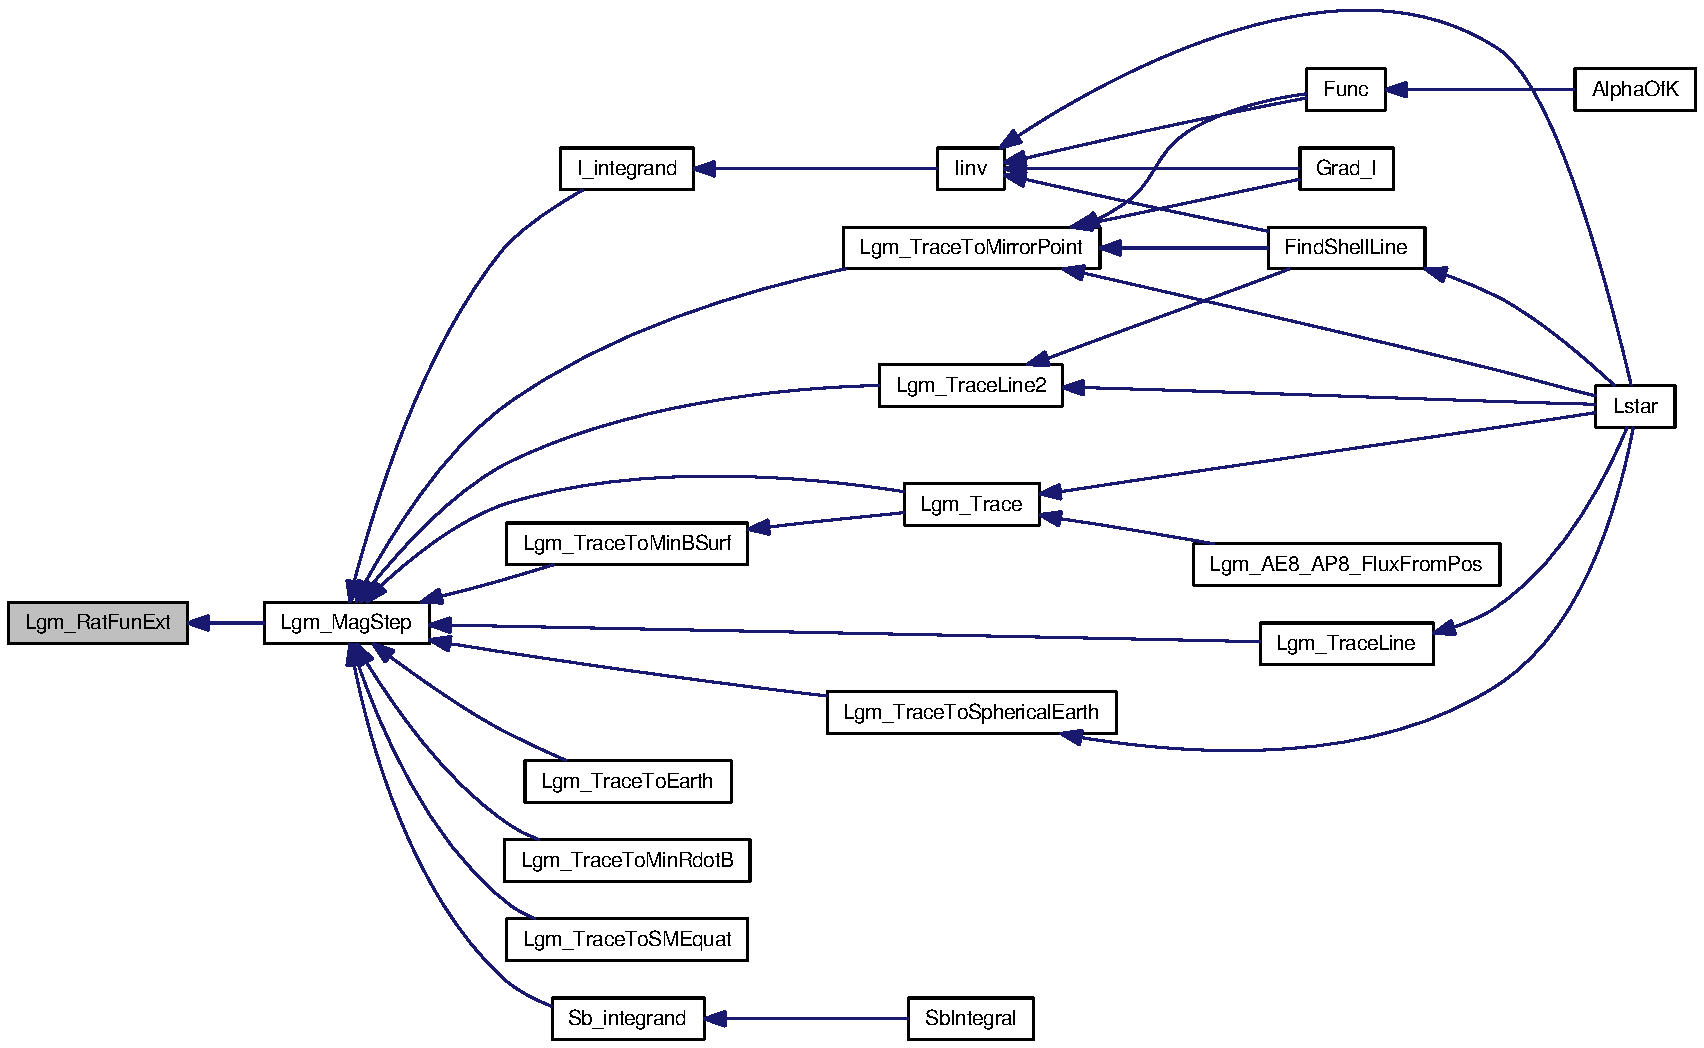
\includegraphics[width=420pt]{_lgm___mag_model_info_8h_1e8a22ce5672e4a4b9a51ca51713408e_icgraph}
\end{center}
\end{figure}
\hypertarget{_lgm___mag_model_info_8h_0728ceef72ddab59dac1779e455e554f}{
\index{Lgm\_\-MagModelInfo.h@{Lgm\_\-MagModelInfo.h}!Lgm\_\-MagStep@{Lgm\_\-MagStep}}
\index{Lgm\_\-MagStep@{Lgm\_\-MagStep}!Lgm_MagModelInfo.h@{Lgm\_\-MagModelInfo.h}}
\subsubsection[{Lgm\_\-MagStep}]{\setlength{\rightskip}{0pt plus 5cm}int Lgm\_\-MagStep ({\bf Lgm\_\-Vector} $\ast$, \/  {\bf Lgm\_\-Vector} $\ast$, \/  double, \/  double $\ast$, \/  double $\ast$, \/  double, \/  double, \/  double $\ast$, \/  int $\ast$, \/  int($\ast$)({\bf Lgm\_\-Vector} $\ast$, {\bf Lgm\_\-Vector} $\ast$, {\bf Lgm\_\-MagModelInfo} $\ast$) {\em Mag}, \/  {\bf Lgm\_\-MagModelInfo} $\ast$)}}
\label{_lgm___mag_model_info_8h_0728ceef72ddab59dac1779e455e554f}




Definition at line 157 of file MagStep.c.

Here is the call graph for this function:\nopagebreak
\begin{figure}[H]
\begin{center}
\leavevmode
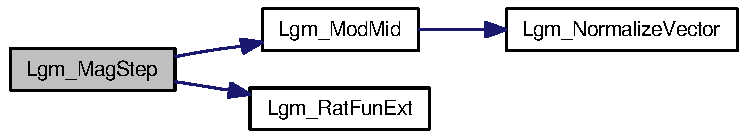
\includegraphics[width=197pt]{_lgm___mag_model_info_8h_0728ceef72ddab59dac1779e455e554f_cgraph}
\end{center}
\end{figure}


Here is the caller graph for this function:\nopagebreak
\begin{figure}[H]
\begin{center}
\leavevmode
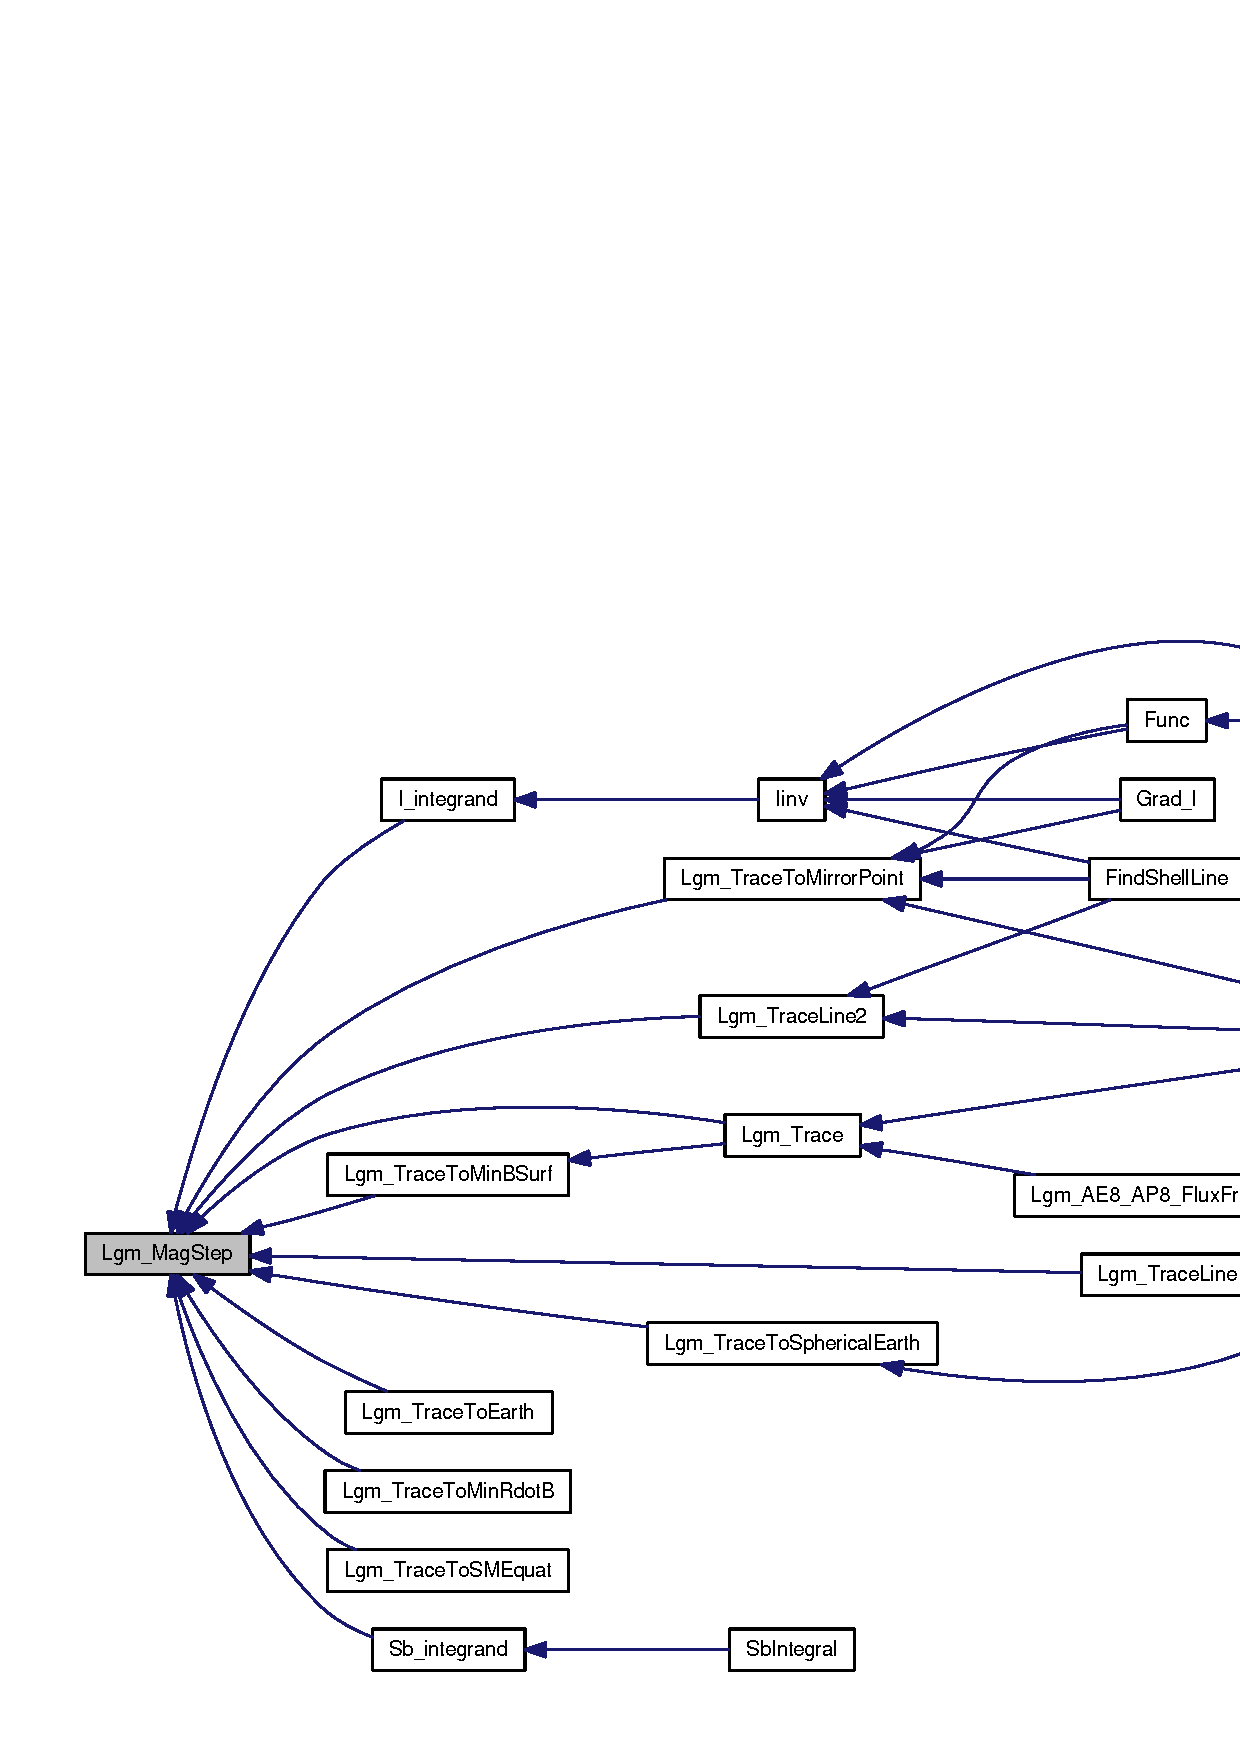
\includegraphics[width=366pt]{_lgm___mag_model_info_8h_0728ceef72ddab59dac1779e455e554f_icgraph}
\end{center}
\end{figure}
\hypertarget{_lgm___mag_model_info_8h_ab7ce7544097d19271704d13d37c95e8}{
\index{Lgm\_\-MagModelInfo.h@{Lgm\_\-MagModelInfo.h}!Lgm\_\-B\_\-igrf@{Lgm\_\-B\_\-igrf}}
\index{Lgm\_\-B\_\-igrf@{Lgm\_\-B\_\-igrf}!Lgm_MagModelInfo.h@{Lgm\_\-MagModelInfo.h}}
\subsubsection[{Lgm\_\-B\_\-igrf}]{\setlength{\rightskip}{0pt plus 5cm}int Lgm\_\-B\_\-igrf ({\bf Lgm\_\-Vector} $\ast$, \/  {\bf Lgm\_\-Vector} $\ast$, \/  {\bf Lgm\_\-MagModelInfo} $\ast$)}}
\label{_lgm___mag_model_info_8h_ab7ce7544097d19271704d13d37c95e8}




Definition at line 3 of file Lgm\_\-B\_\-internal.c.

Here is the call graph for this function:\nopagebreak
\begin{figure}[H]
\begin{center}
\leavevmode
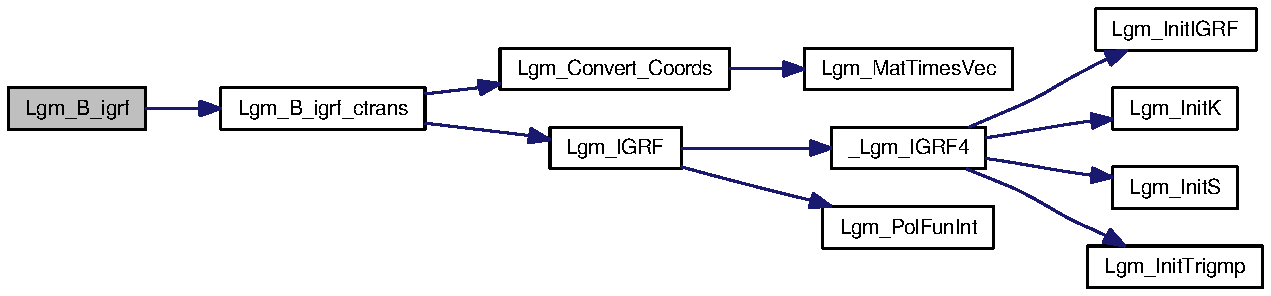
\includegraphics[width=323pt]{_lgm___mag_model_info_8h_ab7ce7544097d19271704d13d37c95e8_cgraph}
\end{center}
\end{figure}


Here is the caller graph for this function:\nopagebreak
\begin{figure}[H]
\begin{center}
\leavevmode
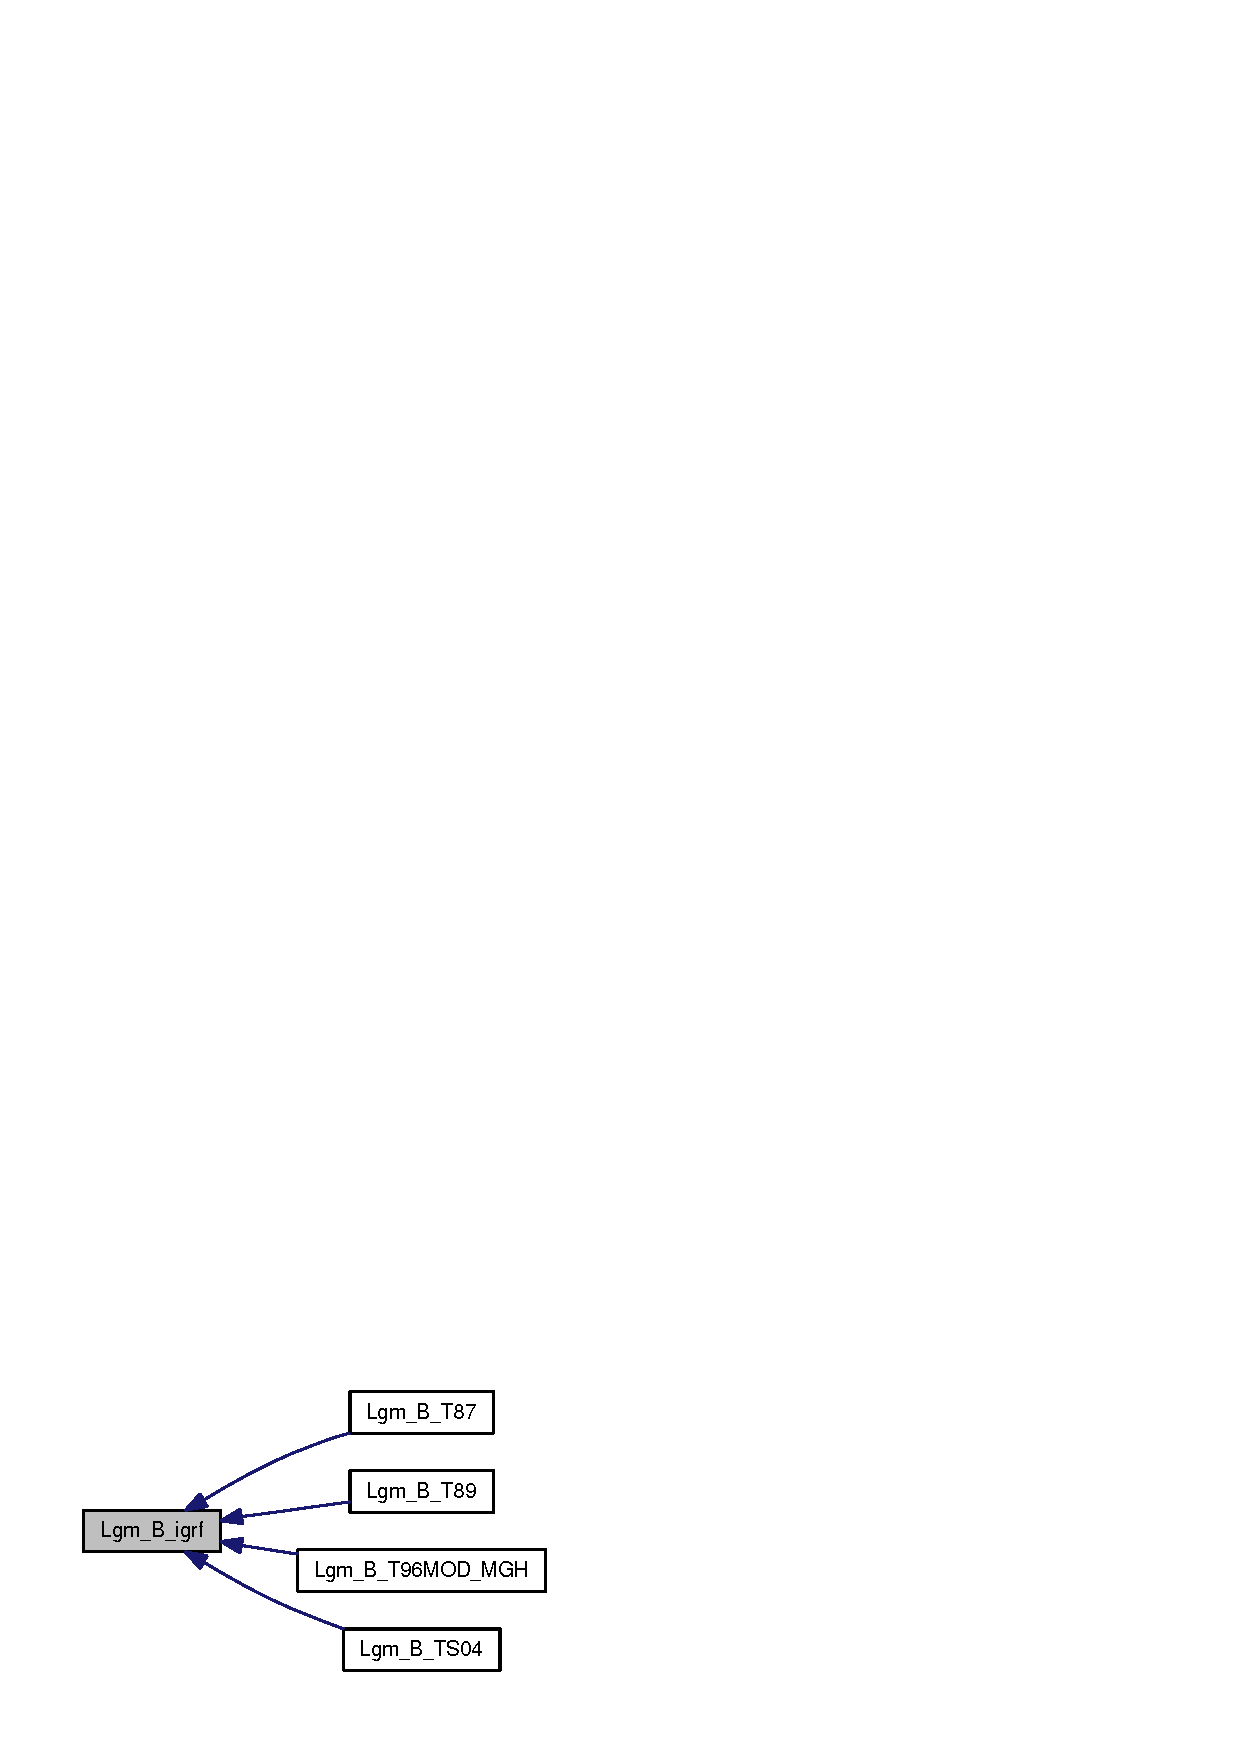
\includegraphics[width=133pt]{_lgm___mag_model_info_8h_ab7ce7544097d19271704d13d37c95e8_icgraph}
\end{center}
\end{figure}
\hypertarget{_lgm___mag_model_info_8h_35a01e17f8707981772eea21f9030af3}{
\index{Lgm\_\-MagModelInfo.h@{Lgm\_\-MagModelInfo.h}!Lgm\_\-B\_\-cdip@{Lgm\_\-B\_\-cdip}}
\index{Lgm\_\-B\_\-cdip@{Lgm\_\-B\_\-cdip}!Lgm_MagModelInfo.h@{Lgm\_\-MagModelInfo.h}}
\subsubsection[{Lgm\_\-B\_\-cdip}]{\setlength{\rightskip}{0pt plus 5cm}int Lgm\_\-B\_\-cdip ({\bf Lgm\_\-Vector} $\ast$, \/  {\bf Lgm\_\-Vector} $\ast$, \/  {\bf Lgm\_\-MagModelInfo} $\ast$)}}
\label{_lgm___mag_model_info_8h_35a01e17f8707981772eea21f9030af3}




Definition at line 8 of file Lgm\_\-B\_\-internal.c.

Here is the call graph for this function:\nopagebreak
\begin{figure}[H]
\begin{center}
\leavevmode
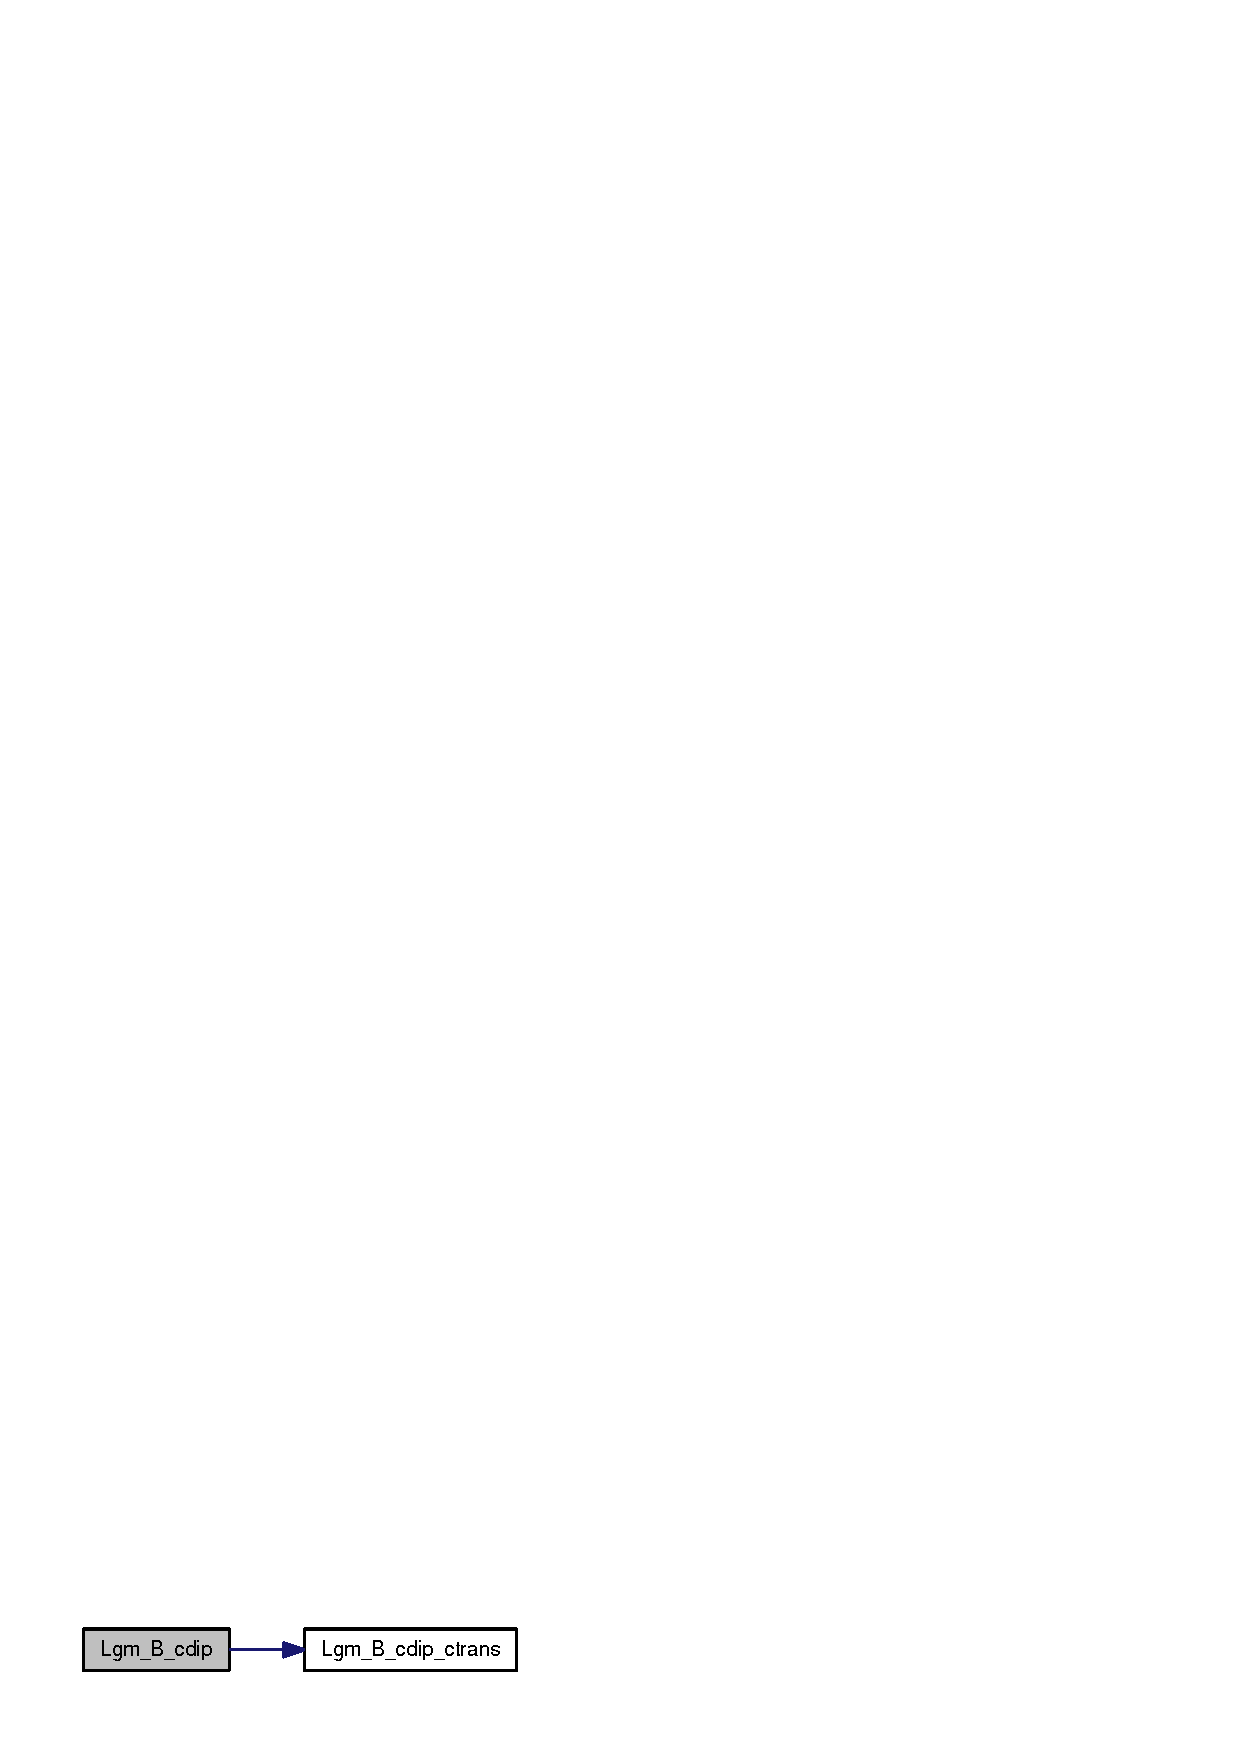
\includegraphics[width=126pt]{_lgm___mag_model_info_8h_35a01e17f8707981772eea21f9030af3_cgraph}
\end{center}
\end{figure}


Here is the caller graph for this function:\nopagebreak
\begin{figure}[H]
\begin{center}
\leavevmode
\includegraphics[width=390pt]{_lgm___mag_model_info_8h_35a01e17f8707981772eea21f9030af3_icgraph}
\end{center}
\end{figure}
\hypertarget{_lgm___mag_model_info_8h_197f94b29b1159e249e52d11d5aec2a8}{
\index{Lgm\_\-MagModelInfo.h@{Lgm\_\-MagModelInfo.h}!Lgm\_\-B\_\-edip@{Lgm\_\-B\_\-edip}}
\index{Lgm\_\-B\_\-edip@{Lgm\_\-B\_\-edip}!Lgm_MagModelInfo.h@{Lgm\_\-MagModelInfo.h}}
\subsubsection[{Lgm\_\-B\_\-edip}]{\setlength{\rightskip}{0pt plus 5cm}int Lgm\_\-B\_\-edip ({\bf Lgm\_\-Vector} $\ast$, \/  {\bf Lgm\_\-Vector} $\ast$, \/  {\bf Lgm\_\-MagModelInfo} $\ast$)}}
\label{_lgm___mag_model_info_8h_197f94b29b1159e249e52d11d5aec2a8}




Definition at line 13 of file Lgm\_\-B\_\-internal.c.

Here is the call graph for this function:\nopagebreak
\begin{figure}[H]
\begin{center}
\leavevmode
\includegraphics[width=126pt]{_lgm___mag_model_info_8h_197f94b29b1159e249e52d11d5aec2a8_cgraph}
\end{center}
\end{figure}


Here is the caller graph for this function:\nopagebreak
\begin{figure}[H]
\begin{center}
\leavevmode
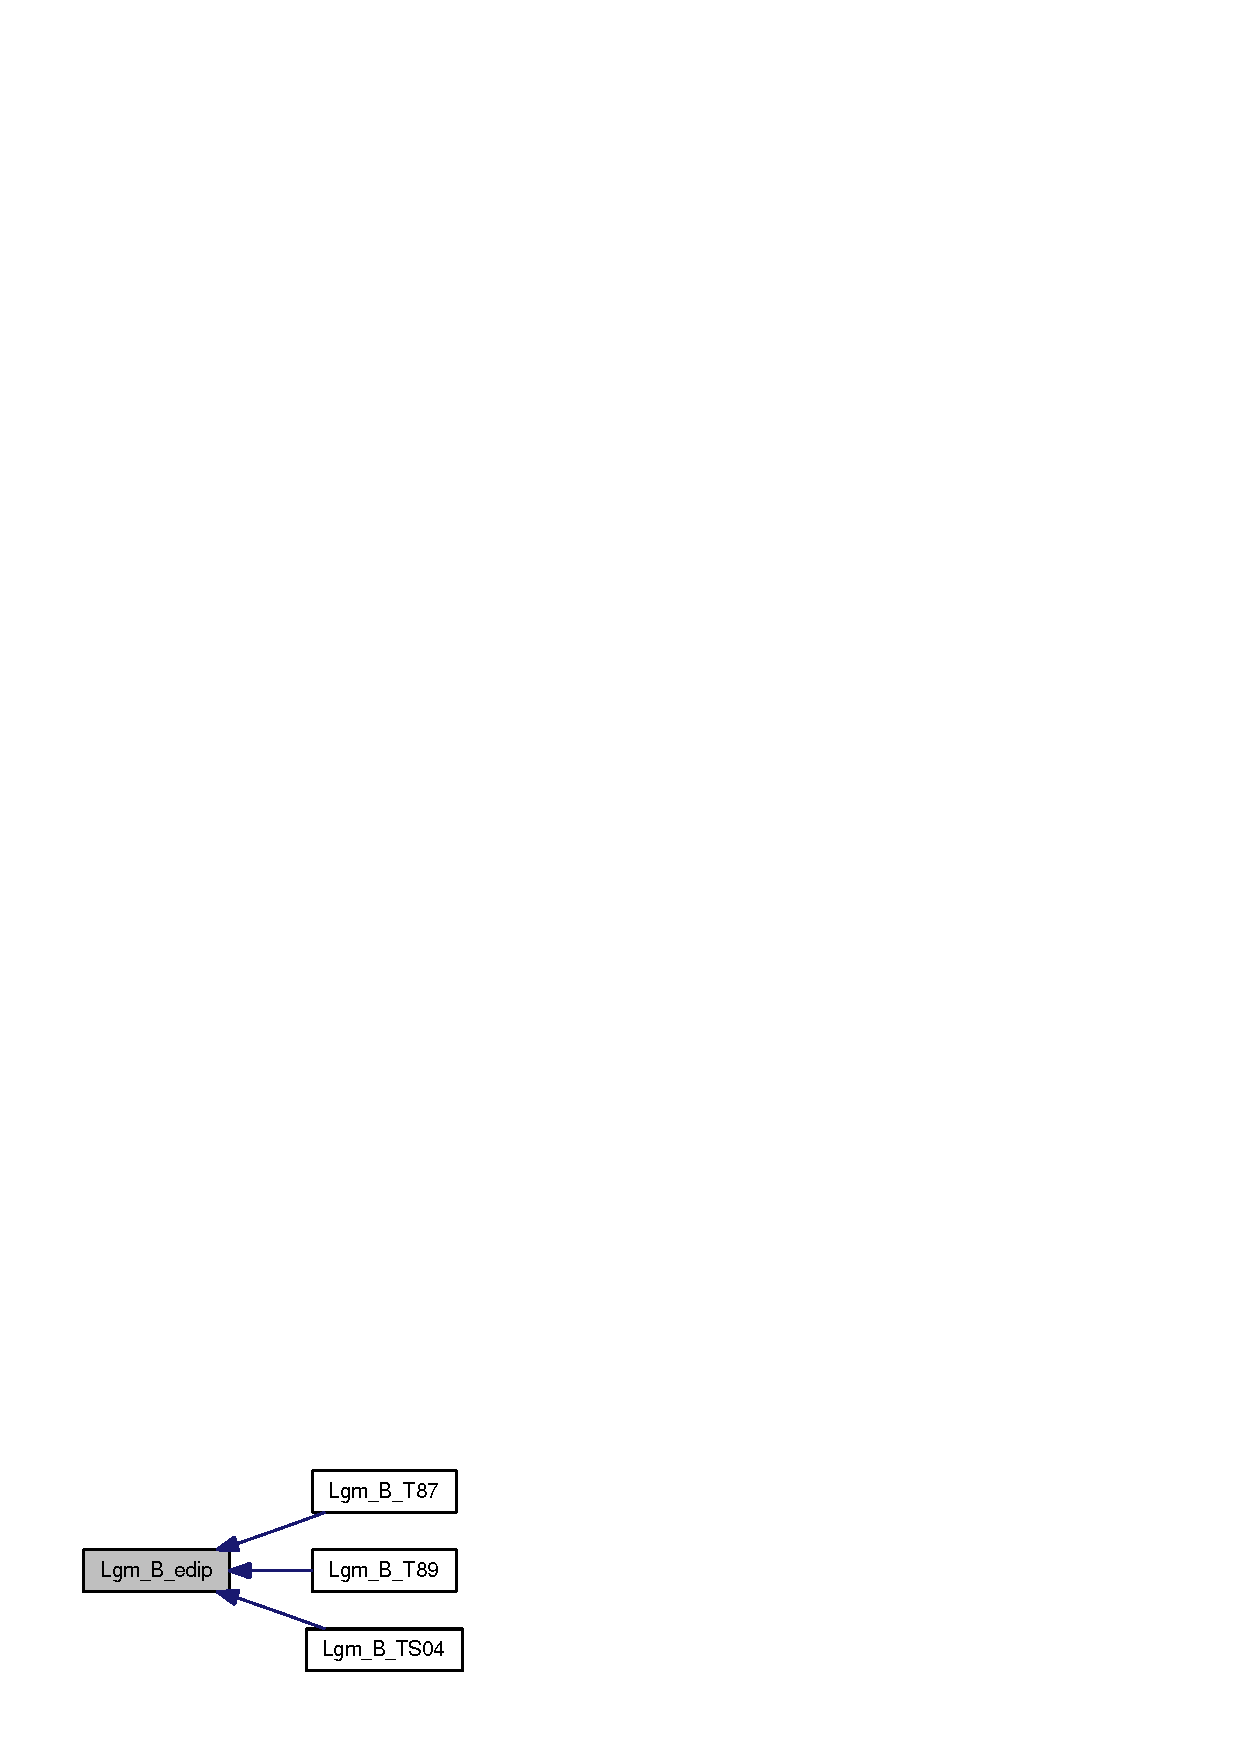
\includegraphics[width=113pt]{_lgm___mag_model_info_8h_197f94b29b1159e249e52d11d5aec2a8_icgraph}
\end{center}
\end{figure}
\hypertarget{_lgm___mag_model_info_8h_1beb428d4ab97b15df348423d1721d90}{
\index{Lgm\_\-MagModelInfo.h@{Lgm\_\-MagModelInfo.h}!Lgm\_\-B1\_\-T87@{Lgm\_\-B1\_\-T87}}
\index{Lgm\_\-B1\_\-T87@{Lgm\_\-B1\_\-T87}!Lgm_MagModelInfo.h@{Lgm\_\-MagModelInfo.h}}
\subsubsection[{Lgm\_\-B1\_\-T87}]{\setlength{\rightskip}{0pt plus 5cm}int Lgm\_\-B1\_\-T87 ({\bf Lgm\_\-Vector} $\ast$, \/  {\bf Lgm\_\-Vector} $\ast$, \/  {\bf Lgm\_\-MagModelInfo} $\ast$)}}
\label{_lgm___mag_model_info_8h_1beb428d4ab97b15df348423d1721d90}




Definition at line 102 of file T87.c.

Here is the caller graph for this function:\nopagebreak
\begin{figure}[H]
\begin{center}
\leavevmode
\includegraphics[width=112pt]{_lgm___mag_model_info_8h_1beb428d4ab97b15df348423d1721d90_icgraph}
\end{center}
\end{figure}
\hypertarget{_lgm___mag_model_info_8h_c500f305bd1f4f0f6bcc61cceb5d300d}{
\index{Lgm\_\-MagModelInfo.h@{Lgm\_\-MagModelInfo.h}!Lgm\_\-B2\_\-T87@{Lgm\_\-B2\_\-T87}}
\index{Lgm\_\-B2\_\-T87@{Lgm\_\-B2\_\-T87}!Lgm_MagModelInfo.h@{Lgm\_\-MagModelInfo.h}}
\subsubsection[{Lgm\_\-B2\_\-T87}]{\setlength{\rightskip}{0pt plus 5cm}int Lgm\_\-B2\_\-T87 ({\bf Lgm\_\-Vector} $\ast$, \/  {\bf Lgm\_\-Vector} $\ast$, \/  {\bf Lgm\_\-MagModelInfo} $\ast$)}}
\label{_lgm___mag_model_info_8h_c500f305bd1f4f0f6bcc61cceb5d300d}




Definition at line 173 of file T87.c.

Here is the caller graph for this function:\nopagebreak
\begin{figure}[H]
\begin{center}
\leavevmode
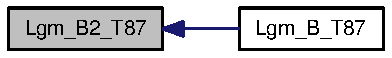
\includegraphics[width=112pt]{_lgm___mag_model_info_8h_c500f305bd1f4f0f6bcc61cceb5d300d_icgraph}
\end{center}
\end{figure}
\hypertarget{_lgm___mag_model_info_8h_884728ac6b23c4a999599757d9a28197}{
\index{Lgm\_\-MagModelInfo.h@{Lgm\_\-MagModelInfo.h}!Lgm\_\-B3\_\-T87@{Lgm\_\-B3\_\-T87}}
\index{Lgm\_\-B3\_\-T87@{Lgm\_\-B3\_\-T87}!Lgm_MagModelInfo.h@{Lgm\_\-MagModelInfo.h}}
\subsubsection[{Lgm\_\-B3\_\-T87}]{\setlength{\rightskip}{0pt plus 5cm}int Lgm\_\-B3\_\-T87 ({\bf Lgm\_\-Vector} $\ast$, \/  {\bf Lgm\_\-Vector} $\ast$, \/  {\bf Lgm\_\-MagModelInfo} $\ast$)}}
\label{_lgm___mag_model_info_8h_884728ac6b23c4a999599757d9a28197}




Definition at line 294 of file T87.c.

Here is the caller graph for this function:\nopagebreak
\begin{figure}[H]
\begin{center}
\leavevmode
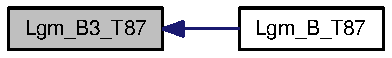
\includegraphics[width=112pt]{_lgm___mag_model_info_8h_884728ac6b23c4a999599757d9a28197_icgraph}
\end{center}
\end{figure}
\hypertarget{_lgm___mag_model_info_8h_642e78d4ec72c24ed023693687d6afb5}{
\index{Lgm\_\-MagModelInfo.h@{Lgm\_\-MagModelInfo.h}!Lgm\_\-B\_\-T87@{Lgm\_\-B\_\-T87}}
\index{Lgm\_\-B\_\-T87@{Lgm\_\-B\_\-T87}!Lgm_MagModelInfo.h@{Lgm\_\-MagModelInfo.h}}
\subsubsection[{Lgm\_\-B\_\-T87}]{\setlength{\rightskip}{0pt plus 5cm}int Lgm\_\-B\_\-T87 ({\bf Lgm\_\-Vector} $\ast$, \/  {\bf Lgm\_\-Vector} $\ast$, \/  {\bf Lgm\_\-MagModelInfo} $\ast$)}}
\label{_lgm___mag_model_info_8h_642e78d4ec72c24ed023693687d6afb5}




Definition at line 325 of file T87.c.

Here is the call graph for this function:\nopagebreak
\begin{figure}[H]
\begin{center}
\leavevmode
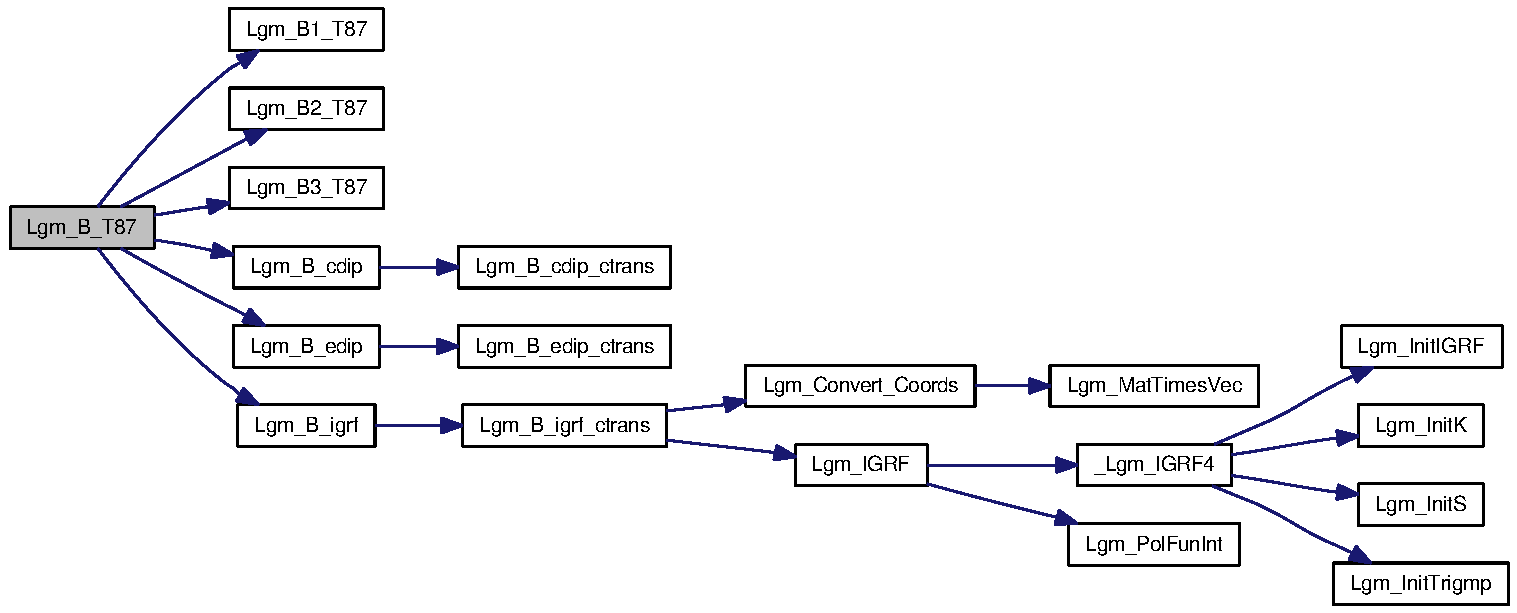
\includegraphics[width=382pt]{_lgm___mag_model_info_8h_642e78d4ec72c24ed023693687d6afb5_cgraph}
\end{center}
\end{figure}
\hypertarget{_lgm___mag_model_info_8h_51eb3ce38725f6f1b611b47b74d8d831}{
\index{Lgm\_\-MagModelInfo.h@{Lgm\_\-MagModelInfo.h}!Lgm\_\-BM\_\-T89@{Lgm\_\-BM\_\-T89}}
\index{Lgm\_\-BM\_\-T89@{Lgm\_\-BM\_\-T89}!Lgm_MagModelInfo.h@{Lgm\_\-MagModelInfo.h}}
\subsubsection[{Lgm\_\-BM\_\-T89}]{\setlength{\rightskip}{0pt plus 5cm}int Lgm\_\-BM\_\-T89 ({\bf Lgm\_\-Vector} $\ast$, \/  {\bf Lgm\_\-Vector} $\ast$, \/  {\bf Lgm\_\-MagModelInfo} $\ast$)}}
\label{_lgm___mag_model_info_8h_51eb3ce38725f6f1b611b47b74d8d831}




Definition at line 322 of file T89.c.

Here is the caller graph for this function:\nopagebreak
\begin{figure}[H]
\begin{center}
\leavevmode
\includegraphics[width=114pt]{_lgm___mag_model_info_8h_51eb3ce38725f6f1b611b47b74d8d831_icgraph}
\end{center}
\end{figure}
\hypertarget{_lgm___mag_model_info_8h_da0b31e3edf146da2f49f5088e4a20ba}{
\index{Lgm\_\-MagModelInfo.h@{Lgm\_\-MagModelInfo.h}!Lgm\_\-BT\_\-T89@{Lgm\_\-BT\_\-T89}}
\index{Lgm\_\-BT\_\-T89@{Lgm\_\-BT\_\-T89}!Lgm_MagModelInfo.h@{Lgm\_\-MagModelInfo.h}}
\subsubsection[{Lgm\_\-BT\_\-T89}]{\setlength{\rightskip}{0pt plus 5cm}int Lgm\_\-BT\_\-T89 ({\bf Lgm\_\-Vector} $\ast$, \/  {\bf Lgm\_\-Vector} $\ast$, \/  {\bf Lgm\_\-MagModelInfo} $\ast$)}}
\label{_lgm___mag_model_info_8h_da0b31e3edf146da2f49f5088e4a20ba}




Definition at line 93 of file T89.c.

Here is the caller graph for this function:\nopagebreak
\begin{figure}[H]
\begin{center}
\leavevmode
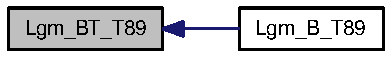
\includegraphics[width=112pt]{_lgm___mag_model_info_8h_da0b31e3edf146da2f49f5088e4a20ba_icgraph}
\end{center}
\end{figure}
\hypertarget{_lgm___mag_model_info_8h_a72b7a373be2bb56c91d7f01eb7661ac}{
\index{Lgm\_\-MagModelInfo.h@{Lgm\_\-MagModelInfo.h}!Lgm\_\-BRC\_\-T89@{Lgm\_\-BRC\_\-T89}}
\index{Lgm\_\-BRC\_\-T89@{Lgm\_\-BRC\_\-T89}!Lgm_MagModelInfo.h@{Lgm\_\-MagModelInfo.h}}
\subsubsection[{Lgm\_\-BRC\_\-T89}]{\setlength{\rightskip}{0pt plus 5cm}int Lgm\_\-BRC\_\-T89 ({\bf Lgm\_\-Vector} $\ast$, \/  {\bf Lgm\_\-Vector} $\ast$, \/  {\bf Lgm\_\-MagModelInfo} $\ast$)}}
\label{_lgm___mag_model_info_8h_a72b7a373be2bb56c91d7f01eb7661ac}




Definition at line 217 of file T89.c.

Here is the caller graph for this function:\nopagebreak
\begin{figure}[H]
\begin{center}
\leavevmode
\includegraphics[width=116pt]{_lgm___mag_model_info_8h_a72b7a373be2bb56c91d7f01eb7661ac_icgraph}
\end{center}
\end{figure}
\hypertarget{_lgm___mag_model_info_8h_478fc5100b3c6a41ed6d6f1bfd833834}{
\index{Lgm\_\-MagModelInfo.h@{Lgm\_\-MagModelInfo.h}!Lgm\_\-BC\_\-T89@{Lgm\_\-BC\_\-T89}}
\index{Lgm\_\-BC\_\-T89@{Lgm\_\-BC\_\-T89}!Lgm_MagModelInfo.h@{Lgm\_\-MagModelInfo.h}}
\subsubsection[{Lgm\_\-BC\_\-T89}]{\setlength{\rightskip}{0pt plus 5cm}int Lgm\_\-BC\_\-T89 ({\bf Lgm\_\-Vector} $\ast$, \/  {\bf Lgm\_\-Vector} $\ast$, \/  {\bf Lgm\_\-MagModelInfo} $\ast$)}}
\label{_lgm___mag_model_info_8h_478fc5100b3c6a41ed6d6f1bfd833834}




Definition at line 348 of file T89.c.

Here is the caller graph for this function:\nopagebreak
\begin{figure}[H]
\begin{center}
\leavevmode
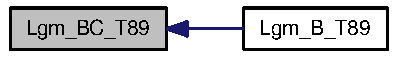
\includegraphics[width=113pt]{_lgm___mag_model_info_8h_478fc5100b3c6a41ed6d6f1bfd833834_icgraph}
\end{center}
\end{figure}
\hypertarget{_lgm___mag_model_info_8h_6faade3e5c2ee066f5d364c1fb4140bb}{
\index{Lgm\_\-MagModelInfo.h@{Lgm\_\-MagModelInfo.h}!Lgm\_\-B\_\-T89@{Lgm\_\-B\_\-T89}}
\index{Lgm\_\-B\_\-T89@{Lgm\_\-B\_\-T89}!Lgm_MagModelInfo.h@{Lgm\_\-MagModelInfo.h}}
\subsubsection[{Lgm\_\-B\_\-T89}]{\setlength{\rightskip}{0pt plus 5cm}int Lgm\_\-B\_\-T89 ({\bf Lgm\_\-Vector} $\ast$, \/  {\bf Lgm\_\-Vector} $\ast$, \/  {\bf Lgm\_\-MagModelInfo} $\ast$)}}
\label{_lgm___mag_model_info_8h_6faade3e5c2ee066f5d364c1fb4140bb}




Definition at line 429 of file T89.c.

Here is the call graph for this function:\nopagebreak
\begin{figure}[H]
\begin{center}
\leavevmode
\includegraphics[width=386pt]{_lgm___mag_model_info_8h_6faade3e5c2ee066f5d364c1fb4140bb_cgraph}
\end{center}
\end{figure}
\hypertarget{_lgm___mag_model_info_8h_6769313ed0ebf3c17cdd0a8491906fc2}{
\index{Lgm\_\-MagModelInfo.h@{Lgm\_\-MagModelInfo.h}!Lgm\_\-B\_\-T96MOD\_\-MGH@{Lgm\_\-B\_\-T96MOD\_\-MGH}}
\index{Lgm\_\-B\_\-T96MOD\_\-MGH@{Lgm\_\-B\_\-T96MOD\_\-MGH}!Lgm_MagModelInfo.h@{Lgm\_\-MagModelInfo.h}}
\subsubsection[{Lgm\_\-B\_\-T96MOD\_\-MGH}]{\setlength{\rightskip}{0pt plus 5cm}int Lgm\_\-B\_\-T96MOD\_\-MGH ({\bf Lgm\_\-Vector} $\ast$ {\em v}, \/  {\bf Lgm\_\-Vector} $\ast$ {\em B}, \/  {\bf Lgm\_\-MagModelInfo} $\ast$ {\em Info})}}
\label{_lgm___mag_model_info_8h_6769313ed0ebf3c17cdd0a8491906fc2}




Definition at line 2 of file T96\_\-MOD\_\-MGH.c.

Here is the call graph for this function:\nopagebreak
\begin{figure}[H]
\begin{center}
\leavevmode
\includegraphics[width=420pt]{_lgm___mag_model_info_8h_6769313ed0ebf3c17cdd0a8491906fc2_cgraph}
\end{center}
\end{figure}
\hypertarget{_lgm___mag_model_info_8h_0a1f7c860cd079e13dedcd24b583bc2b}{
\index{Lgm\_\-MagModelInfo.h@{Lgm\_\-MagModelInfo.h}!lgm\_\-field\_\-t96mod\_\-mgh\_\-@{lgm\_\-field\_\-t96mod\_\-mgh\_\-}}
\index{lgm\_\-field\_\-t96mod\_\-mgh\_\-@{lgm\_\-field\_\-t96mod\_\-mgh\_\-}!Lgm_MagModelInfo.h@{Lgm\_\-MagModelInfo.h}}
\subsubsection[{lgm\_\-field\_\-t96mod\_\-mgh\_\-}]{\setlength{\rightskip}{0pt plus 5cm}void lgm\_\-field\_\-t96mod\_\-mgh\_\- (double $\ast$, \/  double $\ast$, \/  int $\ast$ {\em IYEAR}, \/  int $\ast$ {\em IDAY}, \/  int $\ast$ {\em IH}, \/  int $\ast$ {\em IM}, \/  double $\ast$ {\em SEC}, \/  double $\ast$ {\em X}, \/  double $\ast$ {\em Y}, \/  double $\ast$ {\em Z}, \/  double $\ast$ {\em BX}, \/  double $\ast$ {\em BY}, \/  double $\ast$ {\em BZ})}}
\label{_lgm___mag_model_info_8h_0a1f7c860cd079e13dedcd24b583bc2b}




Here is the caller graph for this function:\nopagebreak
\begin{figure}[H]
\begin{center}
\leavevmode
\includegraphics[width=161pt]{_lgm___mag_model_info_8h_0a1f7c860cd079e13dedcd24b583bc2b_icgraph}
\end{center}
\end{figure}
\hypertarget{_lgm___mag_model_info_8h_e0318c11d75b1133fb52b4393fbe2bea}{
\index{Lgm\_\-MagModelInfo.h@{Lgm\_\-MagModelInfo.h}!lgm\_\-field\_\-t96mod\_\-mgh\_\-\_\-@{lgm\_\-field\_\-t96mod\_\-mgh\_\-\_\-}}
\index{lgm\_\-field\_\-t96mod\_\-mgh\_\-\_\-@{lgm\_\-field\_\-t96mod\_\-mgh\_\-\_\-}!Lgm_MagModelInfo.h@{Lgm\_\-MagModelInfo.h}}
\subsubsection[{lgm\_\-field\_\-t96mod\_\-mgh\_\-\_\-}]{\setlength{\rightskip}{0pt plus 5cm}void lgm\_\-field\_\-t96mod\_\-mgh\_\-\_\- (double $\ast$ {\em PARMOD}, \/  double $\ast$ {\em AMDF}, \/  int $\ast$ {\em IYEAR}, \/  int $\ast$ {\em IDAY}, \/  int $\ast$ {\em IH}, \/  int $\ast$ {\em IM}, \/  double $\ast$ {\em SEC}, \/  double $\ast$ {\em X}, \/  double $\ast$ {\em Y}, \/  double $\ast$ {\em Z}, \/  double $\ast$ {\em BX}, \/  double $\ast$ {\em BY}, \/  double $\ast$ {\em BZ})}}
\label{_lgm___mag_model_info_8h_e0318c11d75b1133fb52b4393fbe2bea}


\hypertarget{_lgm___mag_model_info_8h_2f5583de2b17ada857e7b8d4a50c1c16}{
\index{Lgm\_\-MagModelInfo.h@{Lgm\_\-MagModelInfo.h}!lgm\_\-field\_\-t96mod\_\-@{lgm\_\-field\_\-t96mod\_\-}}
\index{lgm\_\-field\_\-t96mod\_\-@{lgm\_\-field\_\-t96mod\_\-}!Lgm_MagModelInfo.h@{Lgm\_\-MagModelInfo.h}}
\subsubsection[{lgm\_\-field\_\-t96mod\_\-}]{\setlength{\rightskip}{0pt plus 5cm}void lgm\_\-field\_\-t96mod\_\- (int $\ast$, \/  int $\ast$, \/  int $\ast$, \/  int $\ast$, \/  double $\ast$, \/  double $\ast$, \/  double $\ast$, \/  double $\ast$, \/  double $\ast$, \/  double $\ast$, \/  double $\ast$)}}
\label{_lgm___mag_model_info_8h_2f5583de2b17ada857e7b8d4a50c1c16}


\hypertarget{_lgm___mag_model_info_8h_59f3922662b5fde2ade3e5e4a30e33ef}{
\index{Lgm\_\-MagModelInfo.h@{Lgm\_\-MagModelInfo.h}!Lgm\_\-B\_\-TS04@{Lgm\_\-B\_\-TS04}}
\index{Lgm\_\-B\_\-TS04@{Lgm\_\-B\_\-TS04}!Lgm_MagModelInfo.h@{Lgm\_\-MagModelInfo.h}}
\subsubsection[{Lgm\_\-B\_\-TS04}]{\setlength{\rightskip}{0pt plus 5cm}int Lgm\_\-B\_\-TS04 ({\bf Lgm\_\-Vector} $\ast$ {\em v}, \/  {\bf Lgm\_\-Vector} $\ast$ {\em B}, \/  {\bf Lgm\_\-MagModelInfo} $\ast$ {\em Info})}}
\label{_lgm___mag_model_info_8h_59f3922662b5fde2ade3e5e4a30e33ef}




Definition at line 2 of file TS04.c.

Here is the call graph for this function:\nopagebreak
\begin{figure}[H]
\begin{center}
\leavevmode
\includegraphics[width=420pt]{_lgm___mag_model_info_8h_59f3922662b5fde2ade3e5e4a30e33ef_cgraph}
\end{center}
\end{figure}
\hypertarget{_lgm___mag_model_info_8h_0f1aa5cd2fad03bb25ee03b270849fb3}{
\index{Lgm\_\-MagModelInfo.h@{Lgm\_\-MagModelInfo.h}!Lgm\_\-ComputeW@{Lgm\_\-ComputeW}}
\index{Lgm\_\-ComputeW@{Lgm\_\-ComputeW}!Lgm_MagModelInfo.h@{Lgm\_\-MagModelInfo.h}}
\subsubsection[{Lgm\_\-ComputeW}]{\setlength{\rightskip}{0pt plus 5cm}void Lgm\_\-ComputeW (double {\em W}\mbox{[}$\,$\mbox{]}, \/  int {\em i}, \/  double {\em Nk}\mbox{[}$\,$\mbox{]}, \/  double {\em Vk}\mbox{[}$\,$\mbox{]}, \/  double {\em Bsk}\mbox{[}$\,$\mbox{]}, \/  int {\em nk})}}
\label{_lgm___mag_model_info_8h_0f1aa5cd2fad03bb25ee03b270849fb3}




Definition at line 4 of file W.c.\hypertarget{_lgm___mag_model_info_8h_54ecb238c46c4acfe5e022e19cc326ec}{
\index{Lgm\_\-MagModelInfo.h@{Lgm\_\-MagModelInfo.h}!Lgm\_\-T04\_\-s@{Lgm\_\-T04\_\-s}}
\index{Lgm\_\-T04\_\-s@{Lgm\_\-T04\_\-s}!Lgm_MagModelInfo.h@{Lgm\_\-MagModelInfo.h}}
\subsubsection[{Lgm\_\-T04\_\-s}]{\setlength{\rightskip}{0pt plus 5cm}void Lgm\_\-T04\_\-s (int {\em IOPT}, \/  double $\ast$ {\em PARMOD}, \/  double {\em PS}, \/  double {\em SINPS}, \/  double {\em COSPS}, \/  double {\em X}, \/  double {\em Y}, \/  double {\em Z}, \/  double $\ast$ {\em BX}, \/  double $\ast$ {\em BY}, \/  double $\ast$ {\em BZ})}}
\label{_lgm___mag_model_info_8h_54ecb238c46c4acfe5e022e19cc326ec}




Definition at line 198 of file Tsyg2004.c.

Here is the call graph for this function:\nopagebreak
\begin{figure}[H]
\begin{center}
\leavevmode
\includegraphics[width=378pt]{_lgm___mag_model_info_8h_54ecb238c46c4acfe5e022e19cc326ec_cgraph}
\end{center}
\end{figure}


Here is the caller graph for this function:\nopagebreak
\begin{figure}[H]
\begin{center}
\leavevmode
\includegraphics[width=112pt]{_lgm___mag_model_info_8h_54ecb238c46c4acfe5e022e19cc326ec_icgraph}
\end{center}
\end{figure}
\hypertarget{_lgm___mag_model_info_8h_5c047252d169aae0974e5bfed6d71085}{
\index{Lgm\_\-MagModelInfo.h@{Lgm\_\-MagModelInfo.h}!Lgm\_\-EXTERN@{Lgm\_\-EXTERN}}
\index{Lgm\_\-EXTERN@{Lgm\_\-EXTERN}!Lgm_MagModelInfo.h@{Lgm\_\-MagModelInfo.h}}
\subsubsection[{Lgm\_\-EXTERN}]{\setlength{\rightskip}{0pt plus 5cm}void Lgm\_\-EXTERN (int {\em IOPGEN}, \/  int {\em IOPT}, \/  int {\em IOPB}, \/  int {\em IOPR}, \/  double $\ast$ {\em A}, \/  int {\em NTOT}, \/  double {\em PDYN}, \/  double {\em DST}, \/  double {\em BXIMF}, \/  double {\em BYIMF}, \/  double {\em BZIMF}, \/  double {\em W1}, \/  double {\em W2}, \/  double {\em W3}, \/  double {\em W4}, \/  double {\em W5}, \/  double {\em W6}, \/  double {\em PS}, \/  double {\em X}, \/  double {\em Y}, \/  double {\em Z}, \/  double $\ast$ {\em BXCF}, \/  double $\ast$ {\em BYCF}, \/  double $\ast$ {\em BZCF}, \/  double $\ast$ {\em BXT1}, \/  double $\ast$ {\em BYT1}, \/  double $\ast$ {\em BZT1}, \/  double $\ast$ {\em BXT2}, \/  double $\ast$ {\em BYT2}, \/  double $\ast$ {\em BZT2}, \/  double $\ast$ {\em BXSRC}, \/  double $\ast$ {\em BYSRC}, \/  double $\ast$ {\em BZSRC}, \/  double $\ast$ {\em BXPRC}, \/  double $\ast$ {\em BYPRC}, \/  double $\ast$ {\em BZPRC}, \/  double $\ast$ {\em BXR11}, \/  double $\ast$ {\em BYR11}, \/  double $\ast$ {\em BZR11}, \/  double $\ast$ {\em BXR12}, \/  double $\ast$ {\em BYR12}, \/  double $\ast$ {\em BZR12}, \/  double $\ast$ {\em BXR21}, \/  double $\ast$ {\em BYR21}, \/  double $\ast$ {\em BZR21}, \/  double $\ast$ {\em BXR22}, \/  double $\ast$ {\em BYR22}, \/  double $\ast$ {\em BZR22}, \/  double $\ast$ {\em HXIMF}, \/  double $\ast$ {\em HYIMF}, \/  double $\ast$ {\em HZIMF}, \/  double $\ast$ {\em BBX}, \/  double $\ast$ {\em BBY}, \/  double $\ast$ {\em BBZ})}}
\label{_lgm___mag_model_info_8h_5c047252d169aae0974e5bfed6d71085}




Definition at line 302 of file Tsyg2004.c.

Here is the call graph for this function:\nopagebreak
\begin{figure}[H]
\begin{center}
\leavevmode
\includegraphics[width=326pt]{_lgm___mag_model_info_8h_5c047252d169aae0974e5bfed6d71085_cgraph}
\end{center}
\end{figure}


Here is the caller graph for this function:\nopagebreak
\begin{figure}[H]
\begin{center}
\leavevmode
\includegraphics[width=170pt]{_lgm___mag_model_info_8h_5c047252d169aae0974e5bfed6d71085_icgraph}
\end{center}
\end{figure}
\hypertarget{_lgm___mag_model_info_8h_5138e7f3fa8a67aa8ab528ba9cd606d2}{
\index{Lgm\_\-MagModelInfo.h@{Lgm\_\-MagModelInfo.h}!Lgm\_\-B\_\-FromScatteredData@{Lgm\_\-B\_\-FromScatteredData}}
\index{Lgm\_\-B\_\-FromScatteredData@{Lgm\_\-B\_\-FromScatteredData}!Lgm_MagModelInfo.h@{Lgm\_\-MagModelInfo.h}}
\subsubsection[{Lgm\_\-B\_\-FromScatteredData}]{\setlength{\rightskip}{0pt plus 5cm}int Lgm\_\-B\_\-FromScatteredData ({\bf Lgm\_\-Vector} $\ast$ {\em v}, \/  {\bf Lgm\_\-Vector} $\ast$ {\em B}, \/  {\bf Lgm\_\-MagModelInfo} $\ast$ {\em Info})}}
\label{_lgm___mag_model_info_8h_5138e7f3fa8a67aa8ab528ba9cd606d2}




Definition at line 448 of file B\_\-FromScatteredData.c.

Here is the call graph for this function:\nopagebreak
\begin{figure}[H]
\begin{center}
\leavevmode
\includegraphics[width=360pt]{_lgm___mag_model_info_8h_5138e7f3fa8a67aa8ab528ba9cd606d2_cgraph}
\end{center}
\end{figure}
\hypertarget{_lgm___mag_model_info_8h_89bb4edde36de4c65ad855806e4066b3}{
\index{Lgm\_\-MagModelInfo.h@{Lgm\_\-MagModelInfo.h}!Lgm\_\-SimplifiedMead@{Lgm\_\-SimplifiedMead}}
\index{Lgm\_\-SimplifiedMead@{Lgm\_\-SimplifiedMead}!Lgm_MagModelInfo.h@{Lgm\_\-MagModelInfo.h}}
\subsubsection[{Lgm\_\-SimplifiedMead}]{\setlength{\rightskip}{0pt plus 5cm}int Lgm\_\-SimplifiedMead ({\bf Lgm\_\-Vector} $\ast$ {\em v}, \/  {\bf Lgm\_\-Vector} $\ast$ {\em B}, \/  {\bf Lgm\_\-MagModelInfo} $\ast$ {\em Info})}}
\label{_lgm___mag_model_info_8h_89bb4edde36de4c65ad855806e4066b3}




Definition at line 25 of file Lgm\_\-SimplifiedMead.c.\hypertarget{_lgm___mag_model_info_8h_f6e6b0cd75ad626d41e0ce06cbec7320}{
\index{Lgm\_\-MagModelInfo.h@{Lgm\_\-MagModelInfo.h}!Iinv@{Iinv}}
\index{Iinv@{Iinv}!Lgm_MagModelInfo.h@{Lgm\_\-MagModelInfo.h}}
\subsubsection[{Iinv}]{\setlength{\rightskip}{0pt plus 5cm}double Iinv ({\bf Lgm\_\-MagModelInfo} $\ast$ {\em fInfo})}}
\label{_lgm___mag_model_info_8h_f6e6b0cd75ad626d41e0ce06cbec7320}




Definition at line 42 of file IntegralInvariant.c.

Here is the call graph for this function:\nopagebreak
\begin{figure}[H]
\begin{center}
\leavevmode
\includegraphics[width=284pt]{_lgm___mag_model_info_8h_f6e6b0cd75ad626d41e0ce06cbec7320_cgraph}
\end{center}
\end{figure}


Here is the caller graph for this function:\nopagebreak
\begin{figure}[H]
\begin{center}
\leavevmode
\includegraphics[width=141pt]{_lgm___mag_model_info_8h_f6e6b0cd75ad626d41e0ce06cbec7320_icgraph}
\end{center}
\end{figure}
\hypertarget{_lgm___mag_model_info_8h_9378a29574f93271ed37929e9910f6c6}{
\index{Lgm\_\-MagModelInfo.h@{Lgm\_\-MagModelInfo.h}!I\_\-integrand@{I\_\-integrand}}
\index{I\_\-integrand@{I\_\-integrand}!Lgm_MagModelInfo.h@{Lgm\_\-MagModelInfo.h}}
\subsubsection[{I\_\-integrand}]{\setlength{\rightskip}{0pt plus 5cm}double I\_\-integrand (double {\em s}, \/  {\bf \_\-qpInfo} $\ast$ {\em qpInfo})}}
\label{_lgm___mag_model_info_8h_9378a29574f93271ed37929e9910f6c6}




Definition at line 217 of file IntegralInvariant.c.

Here is the call graph for this function:\nopagebreak
\begin{figure}[H]
\begin{center}
\leavevmode
\includegraphics[width=250pt]{_lgm___mag_model_info_8h_9378a29574f93271ed37929e9910f6c6_cgraph}
\end{center}
\end{figure}


Here is the caller graph for this function:\nopagebreak
\begin{figure}[H]
\begin{center}
\leavevmode
\includegraphics[width=191pt]{_lgm___mag_model_info_8h_9378a29574f93271ed37929e9910f6c6_icgraph}
\end{center}
\end{figure}
\hypertarget{_lgm___mag_model_info_8h_ea31055ca3f80f4519c263c09ac3e832}{
\index{Lgm\_\-MagModelInfo.h@{Lgm\_\-MagModelInfo.h}!Iinv\_\-interped@{Iinv\_\-interped}}
\index{Iinv\_\-interped@{Iinv\_\-interped}!Lgm_MagModelInfo.h@{Lgm\_\-MagModelInfo.h}}
\subsubsection[{Iinv\_\-interped}]{\setlength{\rightskip}{0pt plus 5cm}double Iinv\_\-interped ({\bf Lgm\_\-MagModelInfo} $\ast$ {\em fInfo})}}
\label{_lgm___mag_model_info_8h_ea31055ca3f80f4519c263c09ac3e832}




Definition at line 119 of file IntegralInvariant.c.

Here is the call graph for this function:\nopagebreak
\begin{figure}[H]
\begin{center}
\leavevmode
\includegraphics[width=295pt]{_lgm___mag_model_info_8h_ea31055ca3f80f4519c263c09ac3e832_cgraph}
\end{center}
\end{figure}


Here is the caller graph for this function:\nopagebreak
\begin{figure}[H]
\begin{center}
\leavevmode
\includegraphics[width=161pt]{_lgm___mag_model_info_8h_ea31055ca3f80f4519c263c09ac3e832_icgraph}
\end{center}
\end{figure}
\hypertarget{_lgm___mag_model_info_8h_9a3dcc288db0c9c8153abd181494514e}{
\index{Lgm\_\-MagModelInfo.h@{Lgm\_\-MagModelInfo.h}!I\_\-integrand\_\-interped@{I\_\-integrand\_\-interped}}
\index{I\_\-integrand\_\-interped@{I\_\-integrand\_\-interped}!Lgm_MagModelInfo.h@{Lgm\_\-MagModelInfo.h}}
\subsubsection[{I\_\-integrand\_\-interped}]{\setlength{\rightskip}{0pt plus 5cm}double I\_\-integrand\_\-interped (double {\em s}, \/  {\bf \_\-qpInfo} $\ast$ {\em qpInfo})}}
\label{_lgm___mag_model_info_8h_9a3dcc288db0c9c8153abd181494514e}




Definition at line 189 of file IntegralInvariant.c.

Here is the call graph for this function:\nopagebreak
\begin{figure}[H]
\begin{center}
\leavevmode
\includegraphics[width=241pt]{_lgm___mag_model_info_8h_9a3dcc288db0c9c8153abd181494514e_cgraph}
\end{center}
\end{figure}


Here is the caller graph for this function:\nopagebreak
\begin{figure}[H]
\begin{center}
\leavevmode
\includegraphics[width=231pt]{_lgm___mag_model_info_8h_9a3dcc288db0c9c8153abd181494514e_icgraph}
\end{center}
\end{figure}
\hypertarget{_lgm___mag_model_info_8h_64cd517218ca183a56b43dfc1cf7b124}{
\index{Lgm\_\-MagModelInfo.h@{Lgm\_\-MagModelInfo.h}!SbIntegral@{SbIntegral}}
\index{SbIntegral@{SbIntegral}!Lgm_MagModelInfo.h@{Lgm\_\-MagModelInfo.h}}
\subsubsection[{SbIntegral}]{\setlength{\rightskip}{0pt plus 5cm}double SbIntegral ({\bf Lgm\_\-MagModelInfo} $\ast$ {\em fInfo})}}
\label{_lgm___mag_model_info_8h_64cd517218ca183a56b43dfc1cf7b124}




Definition at line 36 of file SbIntegral.c.

Here is the call graph for this function:\nopagebreak
\begin{figure}[H]
\begin{center}
\leavevmode
\includegraphics[width=107pt]{_lgm___mag_model_info_8h_64cd517218ca183a56b43dfc1cf7b124_cgraph}
\end{center}
\end{figure}
\hypertarget{_lgm___mag_model_info_8h_23dd3716fba7aa838e159dbf9f447dd0}{
\index{Lgm\_\-MagModelInfo.h@{Lgm\_\-MagModelInfo.h}!Sb\_\-integrand@{Sb\_\-integrand}}
\index{Sb\_\-integrand@{Sb\_\-integrand}!Lgm_MagModelInfo.h@{Lgm\_\-MagModelInfo.h}}
\subsubsection[{Sb\_\-integrand}]{\setlength{\rightskip}{0pt plus 5cm}double Sb\_\-integrand (double {\em s}, \/  {\bf \_\-qpInfo} $\ast$ {\em qpInfo})}}
\label{_lgm___mag_model_info_8h_23dd3716fba7aa838e159dbf9f447dd0}




Definition at line 174 of file SbIntegral.c.

Here is the call graph for this function:\nopagebreak
\begin{figure}[H]
\begin{center}
\leavevmode
\includegraphics[width=255pt]{_lgm___mag_model_info_8h_23dd3716fba7aa838e159dbf9f447dd0_cgraph}
\end{center}
\end{figure}
\hypertarget{_lgm___mag_model_info_8h_d53ba64293ea16f5d1878d483d62fcd4}{
\index{Lgm\_\-MagModelInfo.h@{Lgm\_\-MagModelInfo.h}!SbIntegral\_\-interped@{SbIntegral\_\-interped}}
\index{SbIntegral\_\-interped@{SbIntegral\_\-interped}!Lgm_MagModelInfo.h@{Lgm\_\-MagModelInfo.h}}
\subsubsection[{SbIntegral\_\-interped}]{\setlength{\rightskip}{0pt plus 5cm}double SbIntegral\_\-interped ({\bf Lgm\_\-MagModelInfo} $\ast$ {\em fInfo})}}
\label{_lgm___mag_model_info_8h_d53ba64293ea16f5d1878d483d62fcd4}




Definition at line 101 of file SbIntegral.c.

Here is the call graph for this function:\nopagebreak
\begin{figure}[H]
\begin{center}
\leavevmode
\includegraphics[width=314pt]{_lgm___mag_model_info_8h_d53ba64293ea16f5d1878d483d62fcd4_cgraph}
\end{center}
\end{figure}
\hypertarget{_lgm___mag_model_info_8h_1828b0051c3925909496a0d956bcaab3}{
\index{Lgm\_\-MagModelInfo.h@{Lgm\_\-MagModelInfo.h}!Sb\_\-integrand\_\-interped@{Sb\_\-integrand\_\-interped}}
\index{Sb\_\-integrand\_\-interped@{Sb\_\-integrand\_\-interped}!Lgm_MagModelInfo.h@{Lgm\_\-MagModelInfo.h}}
\subsubsection[{Sb\_\-integrand\_\-interped}]{\setlength{\rightskip}{0pt plus 5cm}double Sb\_\-integrand\_\-interped (double {\em s}, \/  {\bf \_\-qpInfo} $\ast$ {\em qpInfo})}}
\label{_lgm___mag_model_info_8h_1828b0051c3925909496a0d956bcaab3}




Definition at line 154 of file SbIntegral.c.

Here is the call graph for this function:\nopagebreak
\begin{figure}[H]
\begin{center}
\leavevmode
\includegraphics[width=246pt]{_lgm___mag_model_info_8h_1828b0051c3925909496a0d956bcaab3_cgraph}
\end{center}
\end{figure}


Here is the caller graph for this function:\nopagebreak
\begin{figure}[H]
\begin{center}
\leavevmode
\includegraphics[width=147pt]{_lgm___mag_model_info_8h_1828b0051c3925909496a0d956bcaab3_icgraph}
\end{center}
\end{figure}
\hypertarget{_lgm___mag_model_info_8h_a4b45106bd5072e164b5886359166322}{
\index{Lgm\_\-MagModelInfo.h@{Lgm\_\-MagModelInfo.h}!ratint@{ratint}}
\index{ratint@{ratint}!Lgm_MagModelInfo.h@{Lgm\_\-MagModelInfo.h}}
\subsubsection[{ratint}]{\setlength{\rightskip}{0pt plus 5cm}void ratint (double $\ast$ {\em xa}, \/  double $\ast$ {\em ya}, \/  int {\em n}, \/  double {\em x}, \/  double $\ast$ {\em y}, \/  double $\ast$ {\em dy})}}
\label{_lgm___mag_model_info_8h_a4b45106bd5072e164b5886359166322}


\hypertarget{_lgm___mag_model_info_8h_6b600a2b7549cca974e23521b0412a67}{
\index{Lgm\_\-MagModelInfo.h@{Lgm\_\-MagModelInfo.h}!polint@{polint}}
\index{polint@{polint}!Lgm_MagModelInfo.h@{Lgm\_\-MagModelInfo.h}}
\subsubsection[{polint}]{\setlength{\rightskip}{0pt plus 5cm}void polint (double $\ast$ {\em xa}, \/  double $\ast$ {\em ya}, \/  int {\em n}, \/  double {\em x}, \/  double $\ast$ {\em y}, \/  double $\ast$ {\em dy})}}
\label{_lgm___mag_model_info_8h_6b600a2b7549cca974e23521b0412a67}


\hypertarget{_lgm___mag_model_info_8h_78b06d0a7ba0cb3be1bdf690bf30d21e}{
\index{Lgm\_\-MagModelInfo.h@{Lgm\_\-MagModelInfo.h}!Interp@{Interp}}
\index{Interp@{Interp}!Lgm_MagModelInfo.h@{Lgm\_\-MagModelInfo.h}}
\subsubsection[{Interp}]{\setlength{\rightskip}{0pt plus 5cm}void Interp (double {\em xa}\mbox{[}$\,$\mbox{]}, \/  double {\em ya}\mbox{[}$\,$\mbox{]}, \/  long int {\em n}, \/  double {\em x}, \/  double $\ast$ {\em y})}}
\label{_lgm___mag_model_info_8h_78b06d0a7ba0cb3be1bdf690bf30d21e}


\hypertarget{_lgm___mag_model_info_8h_0990e5337b30952cae12aac2bacf44b3}{
\index{Lgm\_\-MagModelInfo.h@{Lgm\_\-MagModelInfo.h}!Interp2@{Interp2}}
\index{Interp2@{Interp2}!Lgm_MagModelInfo.h@{Lgm\_\-MagModelInfo.h}}
\subsubsection[{Interp2}]{\setlength{\rightskip}{0pt plus 5cm}void Interp2 (double {\em xa}\mbox{[}$\,$\mbox{]}, \/  double {\em ya}\mbox{[}$\,$\mbox{]}, \/  long int {\em n}, \/  double {\em x}, \/  double $\ast$ {\em y})}}
\label{_lgm___mag_model_info_8h_0990e5337b30952cae12aac2bacf44b3}


\hypertarget{_lgm___mag_model_info_8h_ce6dc7c926ea34e07011fb1167c2d5d0}{
\index{Lgm\_\-MagModelInfo.h@{Lgm\_\-MagModelInfo.h}!LFromIBmM\_\-Hilton@{LFromIBmM\_\-Hilton}}
\index{LFromIBmM\_\-Hilton@{LFromIBmM\_\-Hilton}!Lgm_MagModelInfo.h@{Lgm\_\-MagModelInfo.h}}
\subsubsection[{LFromIBmM\_\-Hilton}]{\setlength{\rightskip}{0pt plus 5cm}double LFromIBmM\_\-Hilton (double {\em I}, \/  double {\em Bm}, \/  double {\em M})}}
\label{_lgm___mag_model_info_8h_ce6dc7c926ea34e07011fb1167c2d5d0}




Definition at line 13 of file LFromIBmM.c.

Here is the caller graph for this function:\nopagebreak
\begin{figure}[H]
\begin{center}
\leavevmode
\includegraphics[width=109pt]{_lgm___mag_model_info_8h_ce6dc7c926ea34e07011fb1167c2d5d0_icgraph}
\end{center}
\end{figure}
\hypertarget{_lgm___mag_model_info_8h_3daa38ea6b532d0a030fccd7e8f4d79c}{
\index{Lgm\_\-MagModelInfo.h@{Lgm\_\-MagModelInfo.h}!IFromLBmM\_\-Hilton@{IFromLBmM\_\-Hilton}}
\index{IFromLBmM\_\-Hilton@{IFromLBmM\_\-Hilton}!Lgm_MagModelInfo.h@{Lgm\_\-MagModelInfo.h}}
\subsubsection[{IFromLBmM\_\-Hilton}]{\setlength{\rightskip}{0pt plus 5cm}double IFromLBmM\_\-Hilton (double {\em L}, \/  double {\em Bm}, \/  double {\em M})}}
\label{_lgm___mag_model_info_8h_3daa38ea6b532d0a030fccd7e8f4d79c}




Definition at line 38 of file LFromIBmM.c.\hypertarget{_lgm___mag_model_info_8h_4ee011826916a15076f0efa631ec5e77}{
\index{Lgm\_\-MagModelInfo.h@{Lgm\_\-MagModelInfo.h}!LFromIBmM\_\-McIlwain@{LFromIBmM\_\-McIlwain}}
\index{LFromIBmM\_\-McIlwain@{LFromIBmM\_\-McIlwain}!Lgm_MagModelInfo.h@{Lgm\_\-MagModelInfo.h}}
\subsubsection[{LFromIBmM\_\-McIlwain}]{\setlength{\rightskip}{0pt plus 5cm}double LFromIBmM\_\-McIlwain (double {\em I}, \/  double {\em Bm}, \/  double {\em M})}}
\label{_lgm___mag_model_info_8h_4ee011826916a15076f0efa631ec5e77}




Definition at line 126 of file LFromIBmM.c.

Here is the caller graph for this function:\nopagebreak
\begin{figure}[H]
\begin{center}
\leavevmode
\includegraphics[width=116pt]{_lgm___mag_model_info_8h_4ee011826916a15076f0efa631ec5e77_icgraph}
\end{center}
\end{figure}
\hypertarget{_lgm___mag_model_info_8h_7a35eef2fbb725aae4d03d56ba905dcc}{
\index{Lgm\_\-MagModelInfo.h@{Lgm\_\-MagModelInfo.h}!IFromLBmM\_\-McIlwain@{IFromLBmM\_\-McIlwain}}
\index{IFromLBmM\_\-McIlwain@{IFromLBmM\_\-McIlwain}!Lgm_MagModelInfo.h@{Lgm\_\-MagModelInfo.h}}
\subsubsection[{IFromLBmM\_\-McIlwain}]{\setlength{\rightskip}{0pt plus 5cm}double IFromLBmM\_\-McIlwain (double {\em L}, \/  double {\em Bm}, \/  double {\em M})}}
\label{_lgm___mag_model_info_8h_7a35eef2fbb725aae4d03d56ba905dcc}




Definition at line 175 of file LFromIBmM.c.\hypertarget{_lgm___mag_model_info_8h_be359d7bc7bae132a2e5bff78da3d9b2}{
\index{Lgm\_\-MagModelInfo.h@{Lgm\_\-MagModelInfo.h}!BofS@{BofS}}
\index{BofS@{BofS}!Lgm_MagModelInfo.h@{Lgm\_\-MagModelInfo.h}}
\subsubsection[{BofS}]{\setlength{\rightskip}{0pt plus 5cm}double BofS (double {\em s}, \/  {\bf Lgm\_\-MagModelInfo} $\ast$ {\em Info})}}
\label{_lgm___mag_model_info_8h_be359d7bc7bae132a2e5bff78da3d9b2}




Definition at line 736 of file TraceLine.c.

Here is the call graph for this function:\nopagebreak
\begin{figure}[H]
\begin{center}
\leavevmode
\includegraphics[width=171pt]{_lgm___mag_model_info_8h_be359d7bc7bae132a2e5bff78da3d9b2_cgraph}
\end{center}
\end{figure}


Here is the caller graph for this function:\nopagebreak
\begin{figure}[H]
\begin{center}
\leavevmode
\includegraphics[width=287pt]{_lgm___mag_model_info_8h_be359d7bc7bae132a2e5bff78da3d9b2_icgraph}
\end{center}
\end{figure}
\hypertarget{_lgm___mag_model_info_8h_d90887c3d7981a285406d4a15192ac44}{
\index{Lgm\_\-MagModelInfo.h@{Lgm\_\-MagModelInfo.h}!SofBm@{SofBm}}
\index{SofBm@{SofBm}!Lgm_MagModelInfo.h@{Lgm\_\-MagModelInfo.h}}
\subsubsection[{SofBm}]{\setlength{\rightskip}{0pt plus 5cm}int SofBm (double {\em Bm}, \/  double $\ast$ {\em ss}, \/  double $\ast$ {\em sn}, \/  {\bf Lgm\_\-MagModelInfo} $\ast$ {\em Info})}}
\label{_lgm___mag_model_info_8h_d90887c3d7981a285406d4a15192ac44}




Definition at line 835 of file TraceLine.c.

Here is the call graph for this function:\nopagebreak
\begin{figure}[H]
\begin{center}
\leavevmode
\includegraphics[width=212pt]{_lgm___mag_model_info_8h_d90887c3d7981a285406d4a15192ac44_cgraph}
\end{center}
\end{figure}
\hypertarget{_lgm___mag_model_info_8h_1df3c4796964cae56b6c9bd883d5954b}{
\index{Lgm\_\-MagModelInfo.h@{Lgm\_\-MagModelInfo.h}!Lgm\_\-MagModelInfo\_\-Set\_\-Psw@{Lgm\_\-MagModelInfo\_\-Set\_\-Psw}}
\index{Lgm\_\-MagModelInfo\_\-Set\_\-Psw@{Lgm\_\-MagModelInfo\_\-Set\_\-Psw}!Lgm_MagModelInfo.h@{Lgm\_\-MagModelInfo.h}}
\subsubsection[{Lgm\_\-MagModelInfo\_\-Set\_\-Psw}]{\setlength{\rightskip}{0pt plus 5cm}void Lgm\_\-MagModelInfo\_\-Set\_\-Psw (double {\em Psw}, \/  {\bf Lgm\_\-MagModelInfo} $\ast$ {\em m})}}
\label{_lgm___mag_model_info_8h_1df3c4796964cae56b6c9bd883d5954b}




Definition at line 129 of file Lgm\_\-InitMagInfo.c.\hypertarget{_lgm___mag_model_info_8h_07ff6127e39836ffee154fe3b5eab5e9}{
\index{Lgm\_\-MagModelInfo.h@{Lgm\_\-MagModelInfo.h}!Lgm\_\-MagModelInfo\_\-Set\_\-Kp@{Lgm\_\-MagModelInfo\_\-Set\_\-Kp}}
\index{Lgm\_\-MagModelInfo\_\-Set\_\-Kp@{Lgm\_\-MagModelInfo\_\-Set\_\-Kp}!Lgm_MagModelInfo.h@{Lgm\_\-MagModelInfo.h}}
\subsubsection[{Lgm\_\-MagModelInfo\_\-Set\_\-Kp}]{\setlength{\rightskip}{0pt plus 5cm}void Lgm\_\-MagModelInfo\_\-Set\_\-Kp (double {\em Kp}, \/  {\bf Lgm\_\-MagModelInfo} $\ast$ {\em m})}}
\label{_lgm___mag_model_info_8h_07ff6127e39836ffee154fe3b5eab5e9}




Definition at line 132 of file Lgm\_\-InitMagInfo.c.\hypertarget{_lgm___mag_model_info_8h_c318ccee75354e49cb61fe38ee8d82a4}{
\index{Lgm\_\-MagModelInfo.h@{Lgm\_\-MagModelInfo.h}!Lgm\_\-Set\_\-Octree\_\-kNN\_\-InterpMethod@{Lgm\_\-Set\_\-Octree\_\-kNN\_\-InterpMethod}}
\index{Lgm\_\-Set\_\-Octree\_\-kNN\_\-InterpMethod@{Lgm\_\-Set\_\-Octree\_\-kNN\_\-InterpMethod}!Lgm_MagModelInfo.h@{Lgm\_\-MagModelInfo.h}}
\subsubsection[{Lgm\_\-Set\_\-Octree\_\-kNN\_\-InterpMethod}]{\setlength{\rightskip}{0pt plus 5cm}void Lgm\_\-Set\_\-Octree\_\-kNN\_\-InterpMethod ({\bf Lgm\_\-MagModelInfo} $\ast$ {\em m}, \/  int {\em Method})}}
\label{_lgm___mag_model_info_8h_c318ccee75354e49cb61fe38ee8d82a4}




Definition at line 139 of file Lgm\_\-InitMagInfo.c.\hypertarget{_lgm___mag_model_info_8h_678acc89e6dd0a339e73cd0016d182a8}{
\index{Lgm\_\-MagModelInfo.h@{Lgm\_\-MagModelInfo.h}!Lgm\_\-Set\_\-Octree\_\-kNN\_\-k@{Lgm\_\-Set\_\-Octree\_\-kNN\_\-k}}
\index{Lgm\_\-Set\_\-Octree\_\-kNN\_\-k@{Lgm\_\-Set\_\-Octree\_\-kNN\_\-k}!Lgm_MagModelInfo.h@{Lgm\_\-MagModelInfo.h}}
\subsubsection[{Lgm\_\-Set\_\-Octree\_\-kNN\_\-k}]{\setlength{\rightskip}{0pt plus 5cm}void Lgm\_\-Set\_\-Octree\_\-kNN\_\-k ({\bf Lgm\_\-MagModelInfo} $\ast$ {\em m}, \/  int {\em k})}}
\label{_lgm___mag_model_info_8h_678acc89e6dd0a339e73cd0016d182a8}




Definition at line 143 of file Lgm\_\-InitMagInfo.c.\hypertarget{_lgm___mag_model_info_8h_dbde452adbe800b5292798a1668dd255}{
\index{Lgm\_\-MagModelInfo.h@{Lgm\_\-MagModelInfo.h}!Lgm\_\-Set\_\-Octree\_\-kNN\_\-MaxDist@{Lgm\_\-Set\_\-Octree\_\-kNN\_\-MaxDist}}
\index{Lgm\_\-Set\_\-Octree\_\-kNN\_\-MaxDist@{Lgm\_\-Set\_\-Octree\_\-kNN\_\-MaxDist}!Lgm_MagModelInfo.h@{Lgm\_\-MagModelInfo.h}}
\subsubsection[{Lgm\_\-Set\_\-Octree\_\-kNN\_\-MaxDist}]{\setlength{\rightskip}{0pt plus 5cm}void Lgm\_\-Set\_\-Octree\_\-kNN\_\-MaxDist ({\bf Lgm\_\-MagModelInfo} $\ast$ {\em m}, \/  double {\em MaxDist})}}
\label{_lgm___mag_model_info_8h_dbde452adbe800b5292798a1668dd255}




Definition at line 147 of file Lgm\_\-InitMagInfo.c.\hypertarget{_lgm___mag_model_info_8h_9df19c2b1d0c318e81e774c57ced1929}{
\index{Lgm\_\-MagModelInfo.h@{Lgm\_\-MagModelInfo.h}!Lgm\_\-Set\_\-Open\_\-Limits@{Lgm\_\-Set\_\-Open\_\-Limits}}
\index{Lgm\_\-Set\_\-Open\_\-Limits@{Lgm\_\-Set\_\-Open\_\-Limits}!Lgm_MagModelInfo.h@{Lgm\_\-MagModelInfo.h}}
\subsubsection[{Lgm\_\-Set\_\-Open\_\-Limits}]{\setlength{\rightskip}{0pt plus 5cm}void Lgm\_\-Set\_\-Open\_\-Limits ({\bf Lgm\_\-MagModelInfo} $\ast$ {\em m}, \/  double {\em xmin}, \/  double {\em xmax}, \/  double {\em ymin}, \/  double {\em ymax}, \/  double {\em zmin}, \/  double {\em zmax})}}
\label{_lgm___mag_model_info_8h_9df19c2b1d0c318e81e774c57ced1929}




Definition at line 153 of file Lgm\_\-InitMagInfo.c.

Here is the caller graph for this function:\nopagebreak
\begin{figure}[H]
\begin{center}
\leavevmode
\includegraphics[width=273pt]{_lgm___mag_model_info_8h_9df19c2b1d0c318e81e774c57ced1929_icgraph}
\end{center}
\end{figure}
